\documentclass[fleqn,10pt]{wlscirep}


%\usepackage{hyperref}
\usepackage{epsfig}
\usepackage{bm}
\usepackage{graphicx}
\usepackage{epstopdf}
\usepackage{physics}
\usepackage{siunitx}
\usepackage{colortbl}
\usepackage[super]{nth}
%\usepackage{rotate}
%\usepackage{polyglossia}
%\usepackage{unicode-math}
\usepackage{color}
%\usepackage{fontspec}
\usepackage{subfig}
%\usepackage[affil-it]{authblk}
%\usepackage{fixltx2e}
%\usepackage{dblfloatfix}
\usepackage{bibunits}
\usepackage{amsmath}
\usepackage{mathtools}
\usepackage[left]{lineno}
\usepackage[section]{placeins}




\hypersetup{
    colorlinks=true,       % false: boxed links; true: colored links
    linkcolor=cyan,          % color of internal links
    citecolor=magenta,        % color of links to bibliography
    filecolor=magenta,      % color of file links
    urlcolor=cyan,           % color of external links
    runcolor=cyan
}
\newcommand{\red}[1]{\textcolor{red}{#1}}
\newcommand{\blue}[1]{\textcolor{blue}{#1}}
\newcommand{\figurewidth}{0.8 \columnwidth}
\newcommand{\beqarr}{\begin{eqnarray}}
\newcommand{\eeqarr}{\end{eqnarray}}
\newcommand{\beq}{\begin{equation}}
\newcommand{\eeq}{\end{equation}}
\newcommand{\e}{{\text e}}
\newcommand{\rmd}{{\text d}}
\newcommand{\mc}{\mathcal}
\newcommand{\JJ}[1]{{\textcolor{blue}{[#1]}}}
\newcommand{\DL}[1]{{\textcolor{red}{[DL: #1]}}}
\newcommand{\JR}[1]{{\textcolor{green}{[#1]}}}
\newcommand{\MS}[1]{{\textcolor{orange}{[#1]}}}
\newcommand{\GeV}{\giga\electronvolt}
\newcommand{\TeV}{\tera\electronvolt}
\newcommand{\ignore}[1]{}

%\defaultfontfeatures{Ligatures=TeX,Mapping=tex-text} 
%\setmainfont[Mapping=tex-text]{Palatino}
%\setsansfont[Scale=MatchLowercase,Mapping=tex-text]{Gill Sans}
%\setmonofont[Scale=MatchLowercase]{Andale Mono}
%\defaultbibliography{refs.bib}

\usepackage[printwatermark]{xwatermark}
\usepackage{xcolor}
\usepackage{graphicx}
\usepackage{lipsum}

\title{Solving a Higgs optimization problem with quantum annealing for machine learning}

\author[$^{1\circ}$]{Alex Mott}
\author[$^2$]{Joshua Job}
\author[$^1$]{Jean-Roch Vlimant}
\author[$^3$]{Daniel Lidar}
\author[$^{1*}$]{Maria Spiropulu}
\affil[1]{Department of Physics, California Institute of Technology, Pasadena, 91125, USA }
\affil[2]{Department of Physics,
and Center for Quantum Information Science \& Technology,
University of Southern California, Los Angeles, California 90089, USA}
\affil[3]{Departments of Electrical Engineering, Chemistry and Physics,
and Center for Quantum Information Science \& Technology,
University of Southern California, Los Angeles, California 90089, USA}
\affil[{$^\circ$}]{\small{Now at DeepMind}}
\affil[*]{\small{smaria@caltech.edu}}

%\affil[+]{these authors contributed equally to this work}

\keywords{Higg, quantum annealing, machine learning}



\begin{abstract}


	The discovery of the Higgs boson decays in a background of Standard Model processes was assisted by machine learning methods \cite{Chatrchyan:2012xdj,Aad:2012tfa}. The classifiers used to separate signal from background are trained using  highly unerring but not completely perfect simulations of the physical processes involved, often resulting in label noise and systematic errors. We investigate the application of quantum\cite{kadowaki_quantum_1998,RevModPhys.80.1061,Neven1,Pudenz:2013kx} and classical annealing\cite{kirkpatrick_optimization_1983,katzgraber:06a} in solving a Higgs signal versus background machine learning optimization problem.  We bag a set of weak classifiers built based on the kinematic observables of the Higgs decay photons into a strong classifier that is highly resilient against overtraining and errors in the Monte Carlo simulation correlations of the physics observables. We show that the resulting quantum and classical annealing classifier systems perform comparably to current state of the art machine learning methods used in particle physics\cite{keras,xgboost} and are simple functions of directly interpretable experimental parameters with a clear physical meaning. The annealer-trained classifiers exploit the excited states in the vicinity of the ground state and demonstrate some advantage for small training sizes. This  technique may find application in other areas of experimental particle physics given the algorithm's relative simplicity and robustness to error.
\end{abstract}


%\newwatermark*[allpages,color=red!50,angle=45,scale=3,xpos=0,ypos=0]{DRAFT}
\begin{document}


%  \linenumbers
\flushbottom
\maketitle
%\thispagestyle{empty}
%word count and references for Letter considentation
%\noindent Please note: Abbreviations should be introduced at the first mention in the main text – no abbreviations lists. Suggested structure of main text (not enforced) is provided below.

%\section*{Introduction}
The Higgs boson discovery at the Large Hadron Collider (LHC)~\cite{Chatrchyan:2012xdj,Aad:2012tfa} 
marks the beginning of a new era in Particle Physics.  Experimental particle physicists at the LHC are measuring the new boson's properties~\cite{Khachatryan:2014ira,Aad:2014eha}, searching for heavier Higgs 
bosons\cite{Olive:2016xmw} and trying to understand if the Higgs boson interacts with dark 
matter\cite{Englert:2011yb}. Cosmologists are trying to understand 
the symmetry-breaking Higgs phase transition that took place early in the history of the universe and 
whether that event explains the excess of matter versus antimatter\cite{Morrissey:2012db}. 
Curiously the measured value of the Higgs boson mass~\cite{Olive:2016xmw} tells us that  the symmetry-breaking 
quantum vacuum is metastable\cite{Buttazzo:2013uya} unless new physics intervenes. 
The profound implications of the Higgs boson discovery will keep motivating physics research for the years to come. 

One of the key requirements to precisely measure the properties of the Higgs boson is selecting  
large, high-purity samples containing the production and decay of a Higgs particle.  Applying machine learning techniques~\cite{1742-6596-664-7-072015} is both a potentially powerful approach and offers challenges. The challenge is greater when an investigation requires faithful simulation 
%(using software such as PYTHIA\cite{Pythia:2006} and SHERPA\cite{Sherpa:2009}) 
not only of the physics observables themselves, but also of their correlations in the data.   In the measurement of the properties of the Higgs boson~\cite{Khachatryan:2014ira}, disagreements between simulations and observations result in label noise and systematic uncertainties in the efficiency of the classifiers that adversely impact the classification performance and  translate into uncertainties on the measured properties of the discovered particle.

To address these challenges in the Higgs signal versus background optimization problem we study a binary classifier trained with classical simulated annealing (SA)~\cite{kirkpatrick_optimization_1983,katzgraber:06a} and quantum annealing (QA)~\cite{kadowaki_quantum_1998,RevModPhys.80.1061,Neven1,Pudenz:2013kx,q-sig2}. To implement QA we use a programmable quantum annealer (DW) built by D-Wave Systems, Inc. and housed at the University of Southern California's Information Sciences Institute, comprising 1098 superconducting flux qubits. The optimization problem is mapped to one of finding the ground state of a corresponding Ising spin model. We exploit the excited states in the vicinity of the ground state in the training method to improve the accuracy of the classifiers beyond the baseline ground state finding model. We refer to this  approach as quantum annealing for machine learning (QAML). 


%\section*{Results}:
In what follows we  discuss our results. 
The classifier accuracy is our criterion for comparison between various classifier construction methods.  A classifier that is slow to train may prove practically more useful than a slightly less performant one that is faster to train. 


%\subsection*
We model the Higgs diphoton decay channel $H\rightarrow\gamma\gamma$. See Fig.~\ref{fig:feynman} for the Feynman diagrams of the Higgs production and decay processes. We can represent this system via the momentum of the Higgs particle ($H$), the momenta of the two photons ($\gamma$), the angle $\theta$ with the beam axis, and the azimuthal angle $\phi$.
 
More specifically, we select eight of the kinematical variables describing the generated events as the variables for our classifier. The first five are related to the highest ($p_T^1$) and second highest ($p_T^2$) transverse momentum (momentum perpendicular to the axis defined by the colliding protons) of the photon pair: 
 $p_T^1/m_{\gamma\gamma}$, $p_T^2/m_{\gamma\gamma}$, $(p_T^1\pm p_T^2)/m_{\gamma\gamma}$, $p_T^{\gamma\gamma}/m_{\gamma\gamma}$, where $m_{\gamma\gamma}$ is the invariant mass of the diphoton pair and $p_T^{\gamma\gamma}$ is the transverse momentum of the diphoton system. The last three are $\Delta\eta$ of the two photons -- the separation in the pseudorapidity  $\eta = -\log(\tan(\theta/2))$ ($\eta$ is a pseudo-invariant proxy to $\theta$ commonly used in high energy physics), $\Delta R = \sqrt{\Delta\eta^2+\Delta\phi^2}$ -- the sum in quadrature of the separation in $\eta$ and $\phi$ of the two photons, and $\abs{\eta^{\gamma\gamma}}$ -- the $\eta$ value of the diphoton system.
Figure~\ref{fig:kinematic_variables} shows the distribution of these variables for the signal and background datasets. The differences between these distributions are exploited by the classifier  to distinguish the signal from the background. In addition to these eight variables, we incorporate the various products [using certain rules explained in the Supplementary Information (SI)] between said variables, for a total of $36$, given in Table~\ref{tab:kinematic_variables_key}.
 

We construct weak classifiers from our distributions of kinematical variables as shown in Fig.~\ref{fig:kinematic_variables}, and as described in Methods. We build the corresponding Ising problem as follows\cite{Pudenz:2013kx}. Let $\mc{T} = \{\vec{x_\tau}, y_\tau\}$ denote a given set of training events labeled by the index ${\tau}$, where $\vec{x_\tau}$ is a vector collecting the values of each of the variables we use, and $y_\tau =\pm 1$ is a binary label for whether $\vec{x_\tau}$ is signal ($+1$) or background ($-1$).  If $c_i(\vec{x_\tau})=\pm 1/N$ denotes the value of weak classifier $i$ on the event, where $N$ is the number of weak classifiers, equal to the number of spins or qubits, then with $C_{ij} = \sum_\tau c_i(\vec{x_\tau})c_j(\vec{x_\tau})$ and $C_i = \sum_\tau c_i(\vec{x_\tau}) y_\tau$ and a penalty $\lambda>0$ to prevent overtraining, the Ising Hamiltonian is $H = \sum_{i,j} J_{ij} s_i s_j + \sum_i h_i  s_i$, where $s_i=\pm 1$ is the $i^\textrm{th}$ Ising spin variable, $J_{ij} = \frac{1}{4} C_{ij}$ is the coupling between spins $i$ and $j$, and $h_i =  \lambda-C_i+\frac{1}{2}\sum_{j=1} C_{ij}$ is the local field on spin $i$. The problem QA or SA attempt to solve is to minimize $H$ and return the minimizing, ground state spin configuration $\{s^g_i\}_i$. The strong classifier is then constructed as $R(\vec{x}) = \sum_i s^g_i c_i(\vec{x})\in[-1,1]$ for each new event $\vec{x}$ that we wish to classify \cite{Pudenz:2013kx}. We introduce an additional layer in our study by also constructing strong classifiers from excited state spin configurations.


As benchmarks for traditional machine learning methods we train a deep neural net (DNN) using Keras\cite{keras} with the Theano backend,\cite{2016arXiv160502688full} and  an ensemble of boosted decision trees using XGBoost\cite{xgboost}, using optimized choices for training hyperparameters (details of which can be found in the Supplementary Information). 


%\subsection*
{Variable inclusion}:
We compare  the ground state configurations for $\lambda\in\{0.01,0.05,0.1,0.2,0.4,0.8\}$; a larger $\lambda$ implies an increasing penalty against including additional variables, and thus we expect the variables included at $\lambda=0.8$ to be determining the performance of the classifiers. Table~\ref{fig:variableinclusion} presents the relative strength of the variables in determining the classifier performance by showing how often variables are included in the ground state configuration of the full $36$ variable problem derived from $20$ different training sets with $20$k training events each, as a function of the penalty term $\lambda$.   We find that two of the original kinematical variables, $p_T^1$ and $\eta_{\gamma\gamma}$, are never included.  The number of classifiers included in the ground state of all $20$ training samples' corresponding Hamiltonian is $16$ out of $36$ for $\lambda\leq 0.05$ and the following three for $\lambda=0.8$: i) $p_T^2/m_{\gamma\gamma}$, ii) $(\Delta R\, p_T^{\gamma\gamma})^{-1}$, and iii) $p_T^2/p_T^{\gamma\gamma}$. Those three dominate the network performance and they would have been difficult to guess \textit{a priori} in their composite form.  The physical reason for why these variables are important for the classifier can be gleaned from considering the kinematics of the system.  The key difference between an event with a Higgs decaying to two photons and another process that produces two photons in its final state is the production of the heavy particle in the event.  A heavy particle will require considerably more energy to boost perpendicular to the beamline and hence we would expect real Higgs events to have a characteristically lower $p_{T}^{\gamma\gamma}$ than background events.  Since the system with the Higgs has less transverse boost, we would expect the two photons to have similar $p_T$ spectra, and hence the momentum of the sub-leading photon will typically be higher than in those events without the heavy process.  The $p_T$ of the first photon is largely determined by the overall energy available in the collision, which is also set by $m_{\gamma\gamma}$, hence $p_T^1/m_{\gamma\gamma}$ is largely stochastic and provides little discrimination.


%\subsection*
{Classifier performance}:
We estimate the receiver operating characteristic  (ROC) curves on the training set and construct a final output classifier so that for a given signal efficiency $\epsilon_S$ one uses the strong classifier sampled from the annealer which has the maximum background rejection $r_B$. We construct such compound classifiers for both SA and DW using excited states within a fraction $f$ of the ground state energy $E^g$, i.e., all those $\{s_i\}$ returned so that $H(\{s_i\})<(1-f)E^g$ (note that $E^g<0$). SA is used as a natural comparison to DW on these fully connected problems.

In our experiments DW struggles to find the true minimum of the objective function. This is likely a consequence of the fact that the current generation of the DW2X quantum annealers suffers from non-negligible noise on the programmed Hamiltonian.\footnote{The problem of noise is compounded by the relatively sparse graph that requires a chain of qubits to embed the fully-connected logical Hamiltonian. In our case  $12$ qubits are ferromagnetically coupled  to act as a single logical qubit} Therefore we study and  interrogate current-generation quantum annealers and interpret their performance as a lower bound for the performance of future systems with lower noise and denser hardware graphs. 

In Fig.~\ref{fig:rocs}, we plot the ROC curves for each algorithm for $f=0.05$ at training sizes $100$ and $20,000$.  We observe a clear separation between the annealing-based classifiers and the XGB and DNN classifiers, with the advantage for the annealers appearing at the small training size, but disappearing at the large training size. In Fig.~\ref{fig:aurocs}, we plot the area under the ROC curve (AUROC) for various training sizes and $f=0.05$ (the largest value we used)  for each algorithm. An ideal classifier would have an AUROC of $1$. We find that DW and SA have comparable performance, implying high robustness to approximate solutions of the training problem. This feature appears to generalize across QAML domain-applications (in review, by Li, Felice, Rohs, and D.L. (LFRL)).
%~\cite{lidar-bio}. 
Here the  asymptotic performance of the QAML model is achieved with just $1000$ training events, and thereafter the algorithm does not benefit from additional data.  This is not true of DNN or XGB. A notable finding of this work is that QAML has an advantage over both DNN and XGB when training sizes are small. This is shown in Fig.~\ref{fig:audrocs} in terms of the integral of the true negative differences over signal efficiency for various ROCs. In the same regime of small training sizes, DW develops a small advantage over SA as the fraction of excited states $f$ used increases, saturating at $f=0.05$. The uncertainties are too large to draw definitive conclusions in this regard. In the regime of large training sizes, SA has a small advantage over DW, to a significance of approximately $2\sigma$.


%\section*{Discussion}
We proceed to discuss and summarize our results.
With this study we explore QAML, a simple method inspired by the prospect of using quantum annealing as an optimization technique for constructing classifiers, and apply the technique to the detection of Higgs decays. The training data is represented in a compact representation of $\mathcal{O}(N^2)$ couplers and local biases in the Hamiltonian for $N$ weak classifiers.
The resulting strong classifiers perform comparably to the state-of-the-art standard methods used in high energy physics today, and have an advantage when training sizes are small.  The role of QA is that of a subroutine for sampling the Ising problem that may in the future have advantages over classical samplers, either when used directly or as a method of seeding classical solvers with-high quality initial states.

QAML is resistant to overfitting, as the method involves an explicit linearization of correlations. It is also less sensitive to errors in the Monte Carlo correlation estimates than DNNs or binary decision trees due to the truncation of the tails of the distributions (see the Supplementary Information). 
A useful aspect of the model is that it is directly interpretable, as each weak classifier directly corresponds to some physically relevant variable or product or ratio of variables, and the strong classifier is a simple linear combination thereof. This is in contrast to the usual creation of black-box machine learning discriminants, such as when using DNNs and XGBoost, where techniques for interpretability are still an active area of research \cite{Chen:2016aa}. 

This example of using quantum annealing to optimize classifiers in a physics problem is the first to-date, to the best of the authors' knowledge, and it opens further opportunities for research. Quantum machine learning has taken great theoretical strides in the past years  \cite{Lloyd:2014fk,Wiebe:2014vn,Paparo:2014kx,Rebentrost:2014uq,Schuld:2014eu,Cong:2015zr,Biamonte:2016aa} and we demonstrate that we can already apply elements of this technique to current and next-generation quantum annealing architectures. The near future will see applications of these techniques to more complex problems in particle physics and other domain sciences. For example, this work has motivated similar studies in computational biology (in review, LFRL).%~\cite{lidar-bio}.
We envision that QAML could be used further in the context of data certification in high energy physics,
where training with small dataset size could be particularly useful. One can leverage the robustness of QAML to 
both significantly reduce the level of human intervention and increase the accuracy in quickly assessing and certifying the collision data 
for physics analysis. Being impervious to overtraining, QAML is a good candidate for boosting\cite{xgboost}
and we foresee studies to evaluate this using future versions of the D-Wave quantum annealers or other architectures, or even classical optimization techniques such as SA. 
Multi-stage classifiers---where the most influential variables are found via training and pulled out to form a smarter classifier---could be used to mitigate the influence of hardware noise in the quantum annealer.  With more available qubits, or more efficient architectures, integer weights could be used in place of the binary weights through a straightforward extension of the encoding scheme used in this work. 


\section*{Acknowledgements}
This project is supported in part by the  United States Department of Energy, Office of High Energy Physics Research Technology Computational HEP and Fermi Research Alliance, LLC under Contract No. DE-AC02-07CH11359.  The project is also supported in part under ARO grant number W911NF-12-1-0523 and NSF grant number INSPIRE-1551064. The work is supported in part by the AT\&T Foundry Innovation Centers through INQNET, a program for accelerating quantum technologies.  We wish to thank the Advanced Scientific Computing Research program of the DOE for the opportunity to first present and discuss this work at the ASCR workshop on Quantum Computing for Science (2015). We  acknowledge the funding agencies and all the scientists and staff at CERN and internationally whose  hard work resulted in the momentous H(125) discovery in 2012. 

%
%Acknowledgements should be brief, and should not include thanks to anonymous referees and editors, or effusive comments. Grant or contribution numbers may be acknowledged.

\section*{Author contributions statement}
A.M. conducted  the first mapping of the problem on the D-Wave software architecture, data analysis and machine learning methodology,  and along with M.S. provided the core knowledge of the domain science (Higgs physics). J.J conducted  QA and SA  research and data analysis as well as the machine learning work and along with D.L. provided the core of QA/SA knowledge. J-R.V. conducted  QA research, data analysis, machine learning methods and error analysis work with J.J. for the submitted version of the work.  D.L. and M.S. provided the overall oversight and scrutiny of the research work, data analysis and results.  D.L. conceived the quantum machine learning methodology and M.S. conceived the domain application.   We consider the two graduate students (A.M. and J.J.) as operationally the first authors of this work. All authors contributed to writing and reviewing the manuscript. Correspondence and requests for materials should be addressed to Maria Spiropulu at smaria@caltech.edu.
%
%Must include all authors, identified by initials, for example:
%A.A. conceived the experiment(s),  A.A. and B.A. conducted the experiment(s), C.A. and D.A. analysed the results.  All authors reviewed the manuscript. 

\section*{Additional information}
%
%To include, in this order: \textbf{Accession codes} (where applicable); 
\textbf{Competing financial interests}:

The authors declare no competing financial interests.


\FloatBarrier
\newpage\newpage

\begin{figure}
\begin{center}
 	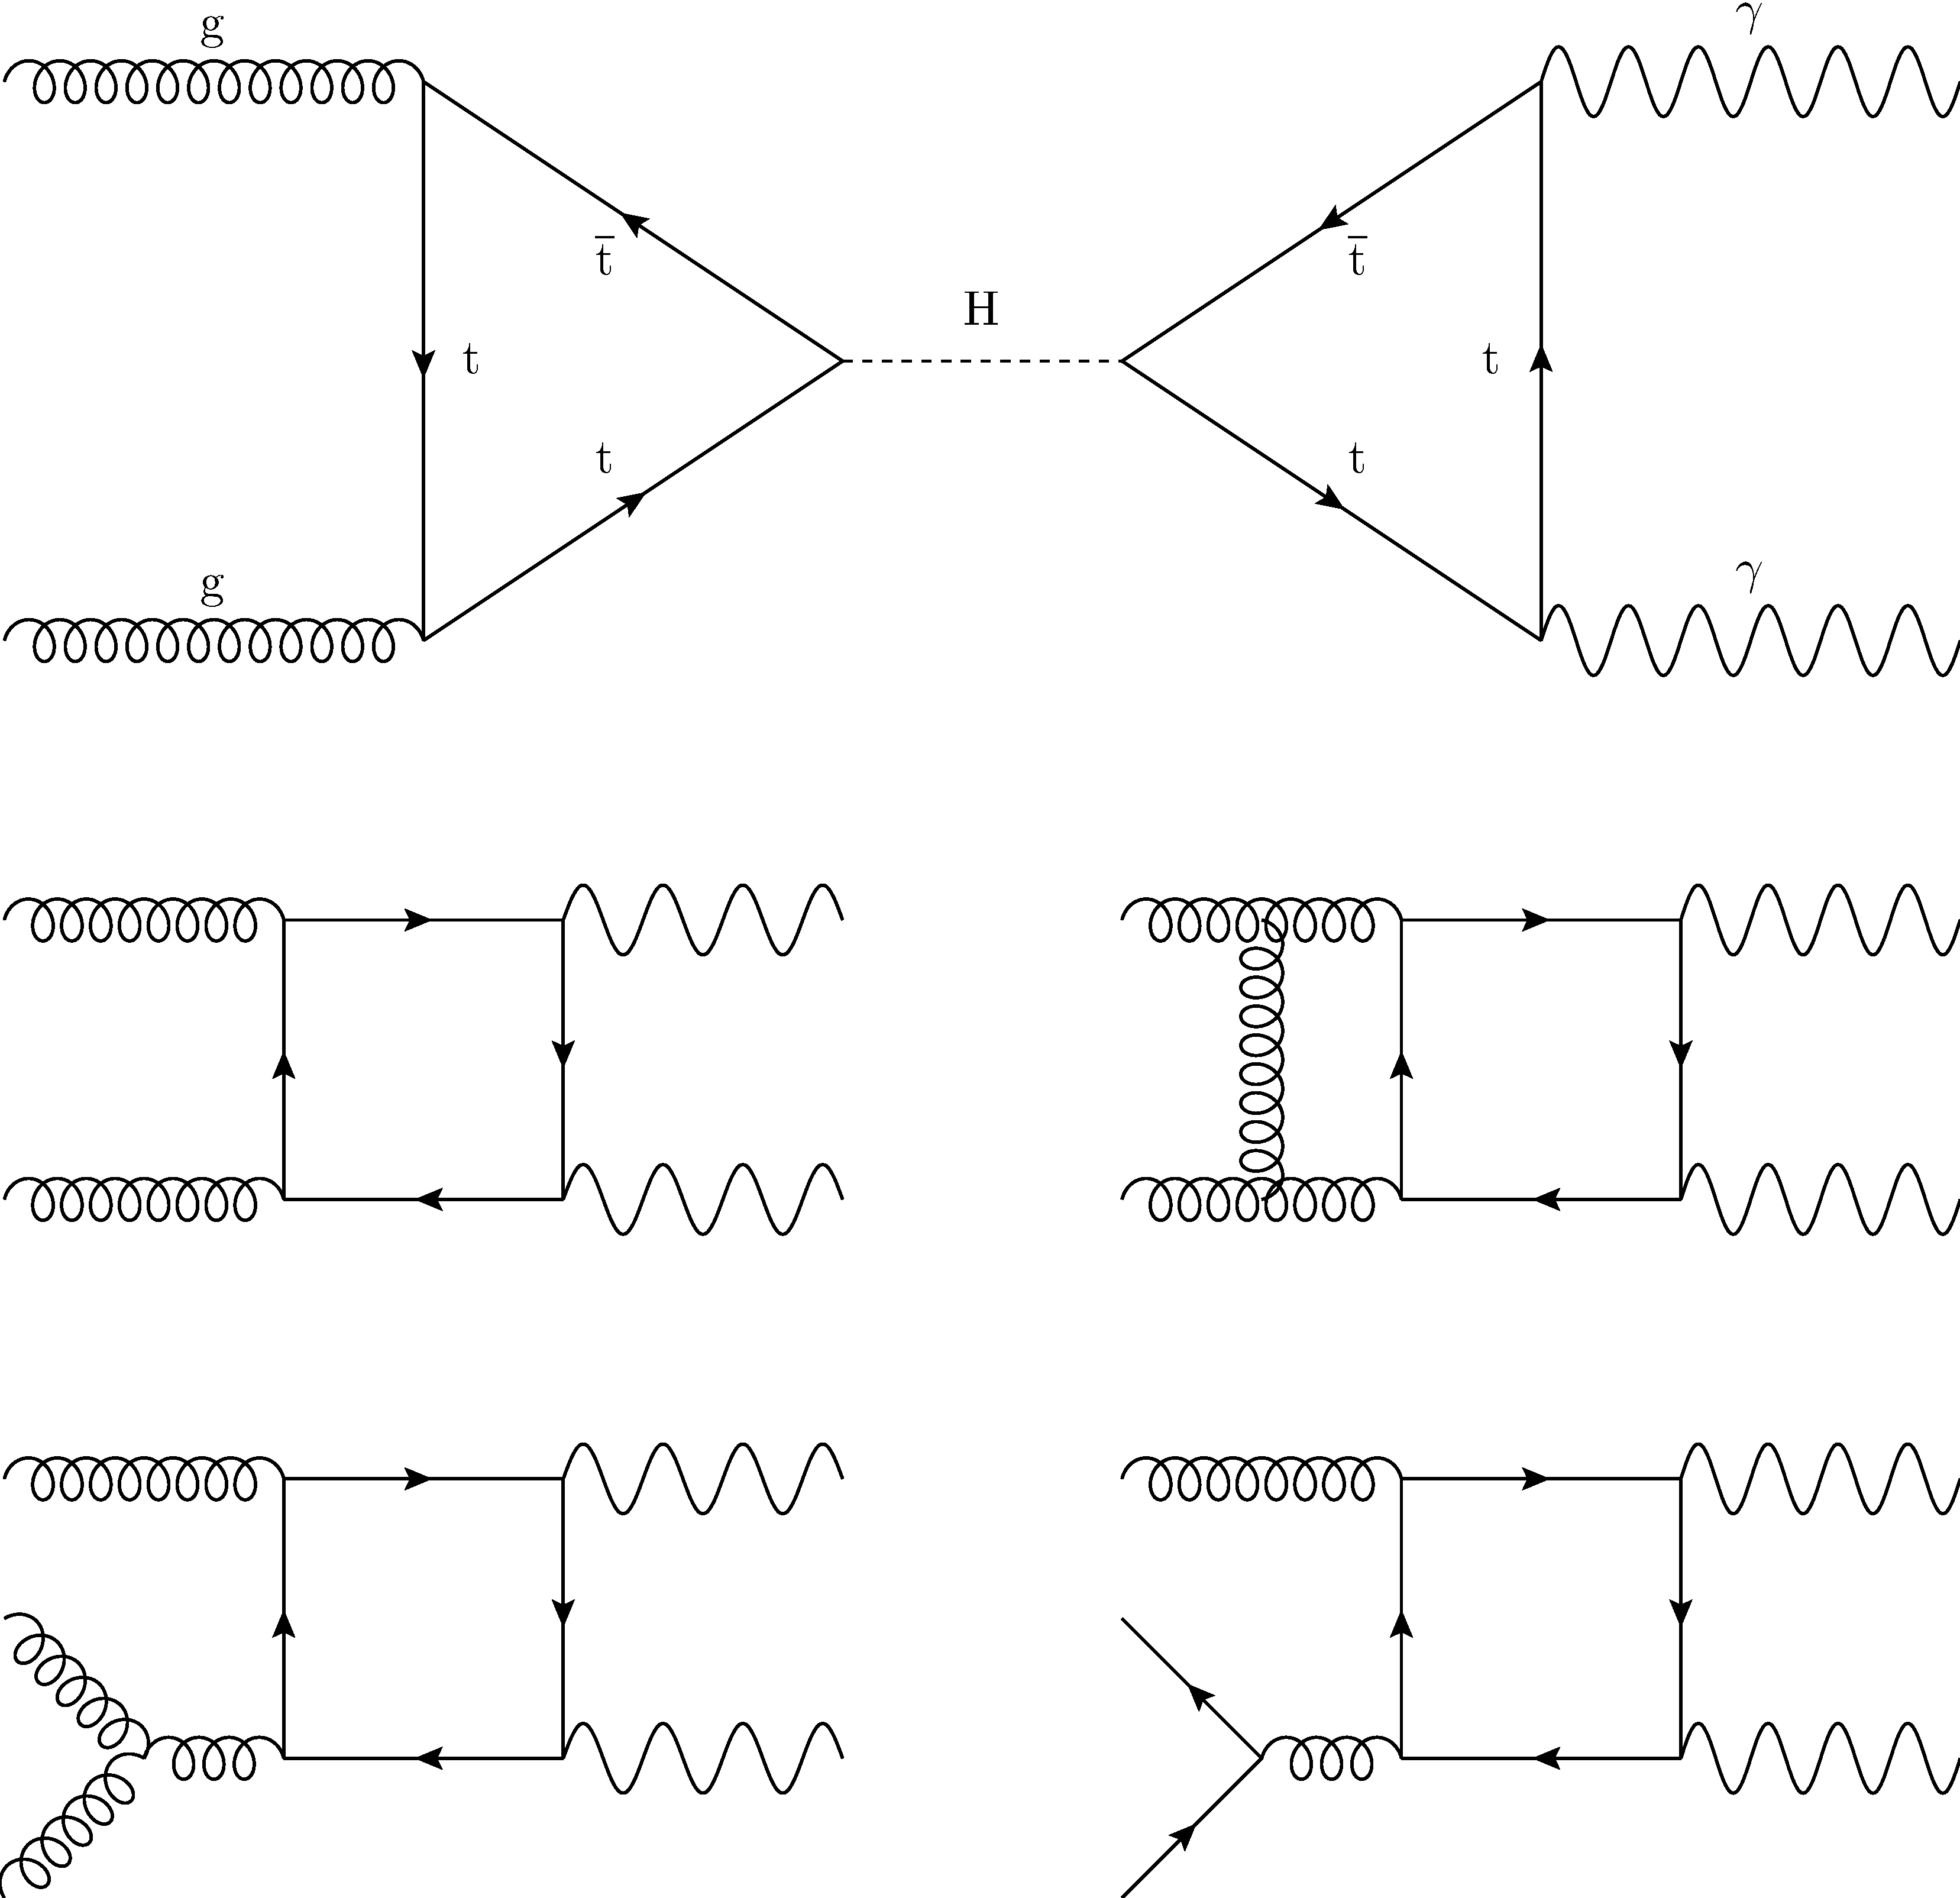
\includegraphics[width=.6\textwidth]{Fig1-Hgg-Xgg.pdf}
	\end{center}
	\caption{\textbf{Representative Feynman diagrams} contributing to the simulated distributions for Higgs signal and Standard Model background. The signal is a Higgs production through gluon-fusion which decays into two photons (top). Representative Leading Order and Next-to-Leading Order  background processes are Standard Model two photon  production  processes (bottom).}
 	\label{fig:feynman}
 \end{figure}

\begin{figure*}[hbt]
 \centering
  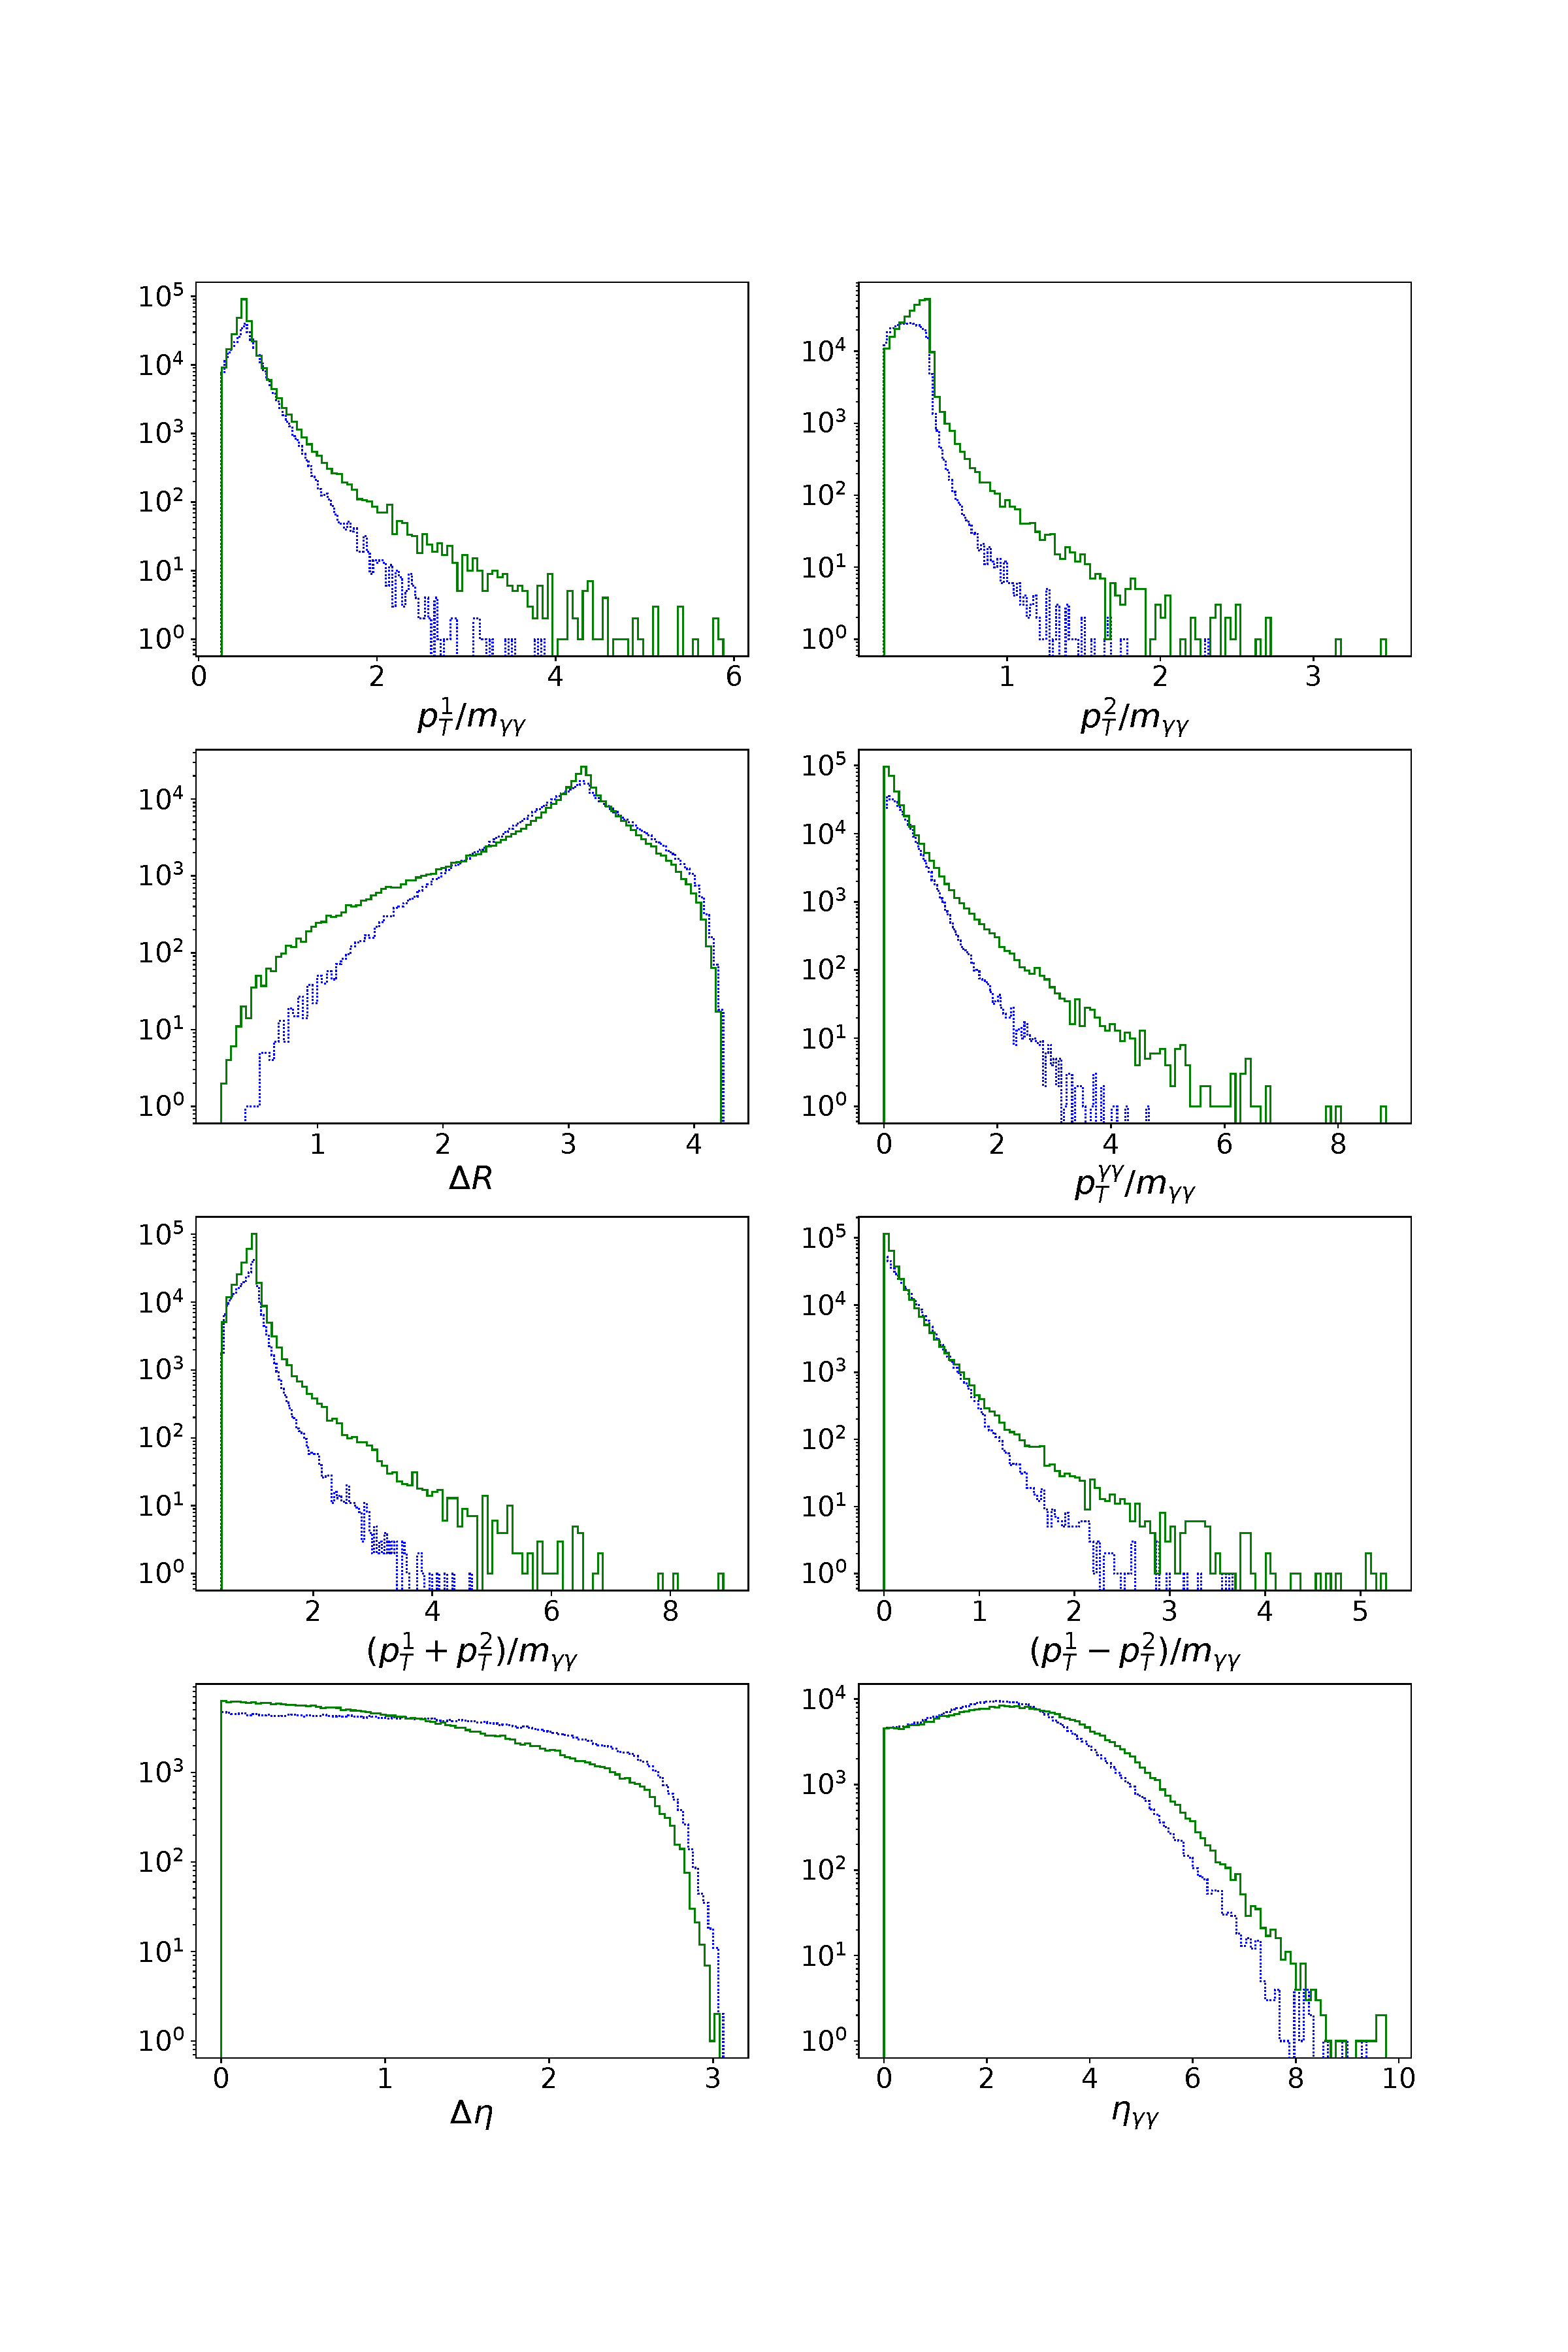
\includegraphics[width=.9\textwidth]{Fig2-kinematical_variables.pdf}
%\vspace{-2.5cm}
\caption{\textbf{Distributions of the eight kinematical variables} we used to construct weak classifiers. The signal distribution is in green and solid, background in blue and dotted. The vertical axis is the raw count of the number of events. The total number of events simulated in each case is $307732$.
 }
  \label{fig:kinematic_variables}
\end{figure*}


 \begin{figure*}[hbt]
  \subfloat[]{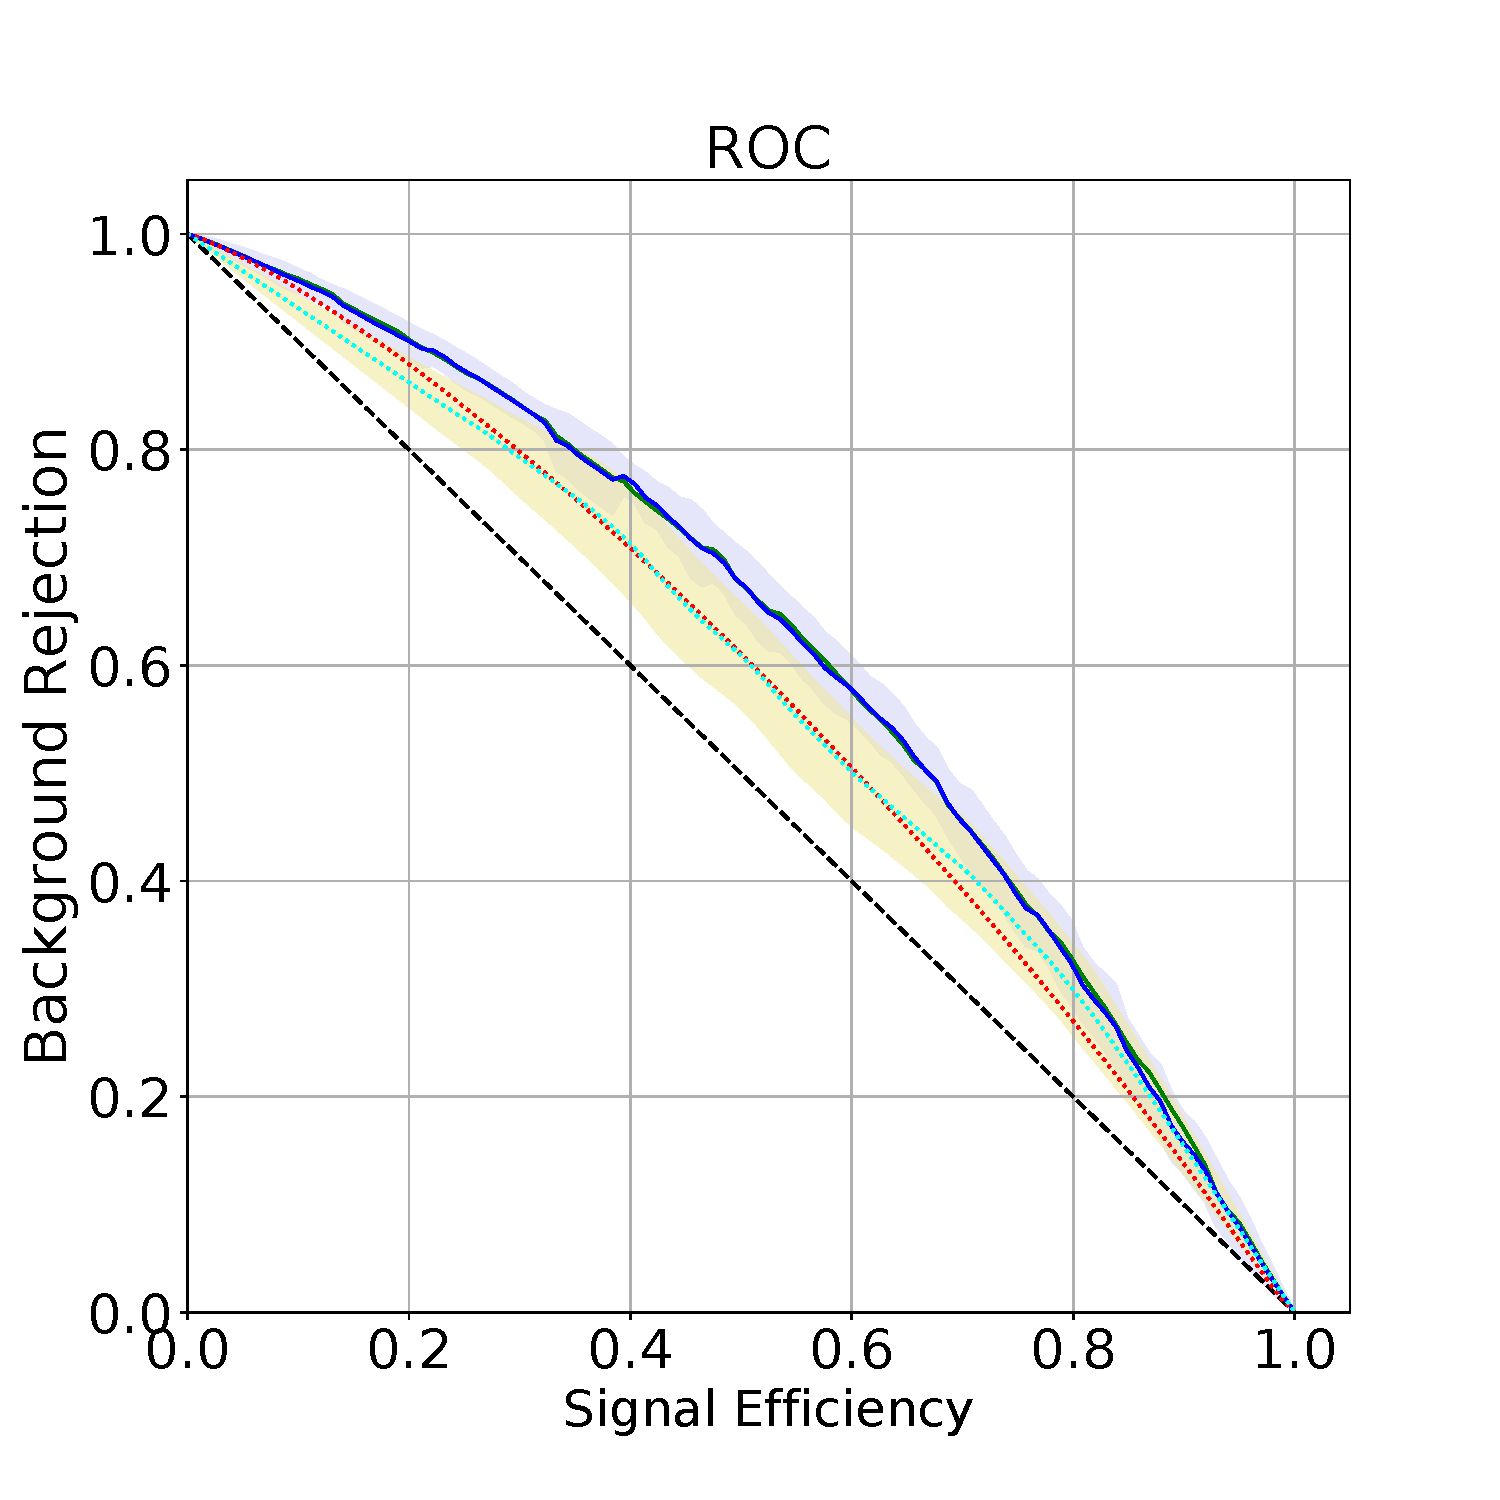
\includegraphics[width=0.5\textwidth]{Fig3a-ROC_example_100DWDNN}}
  \subfloat[]{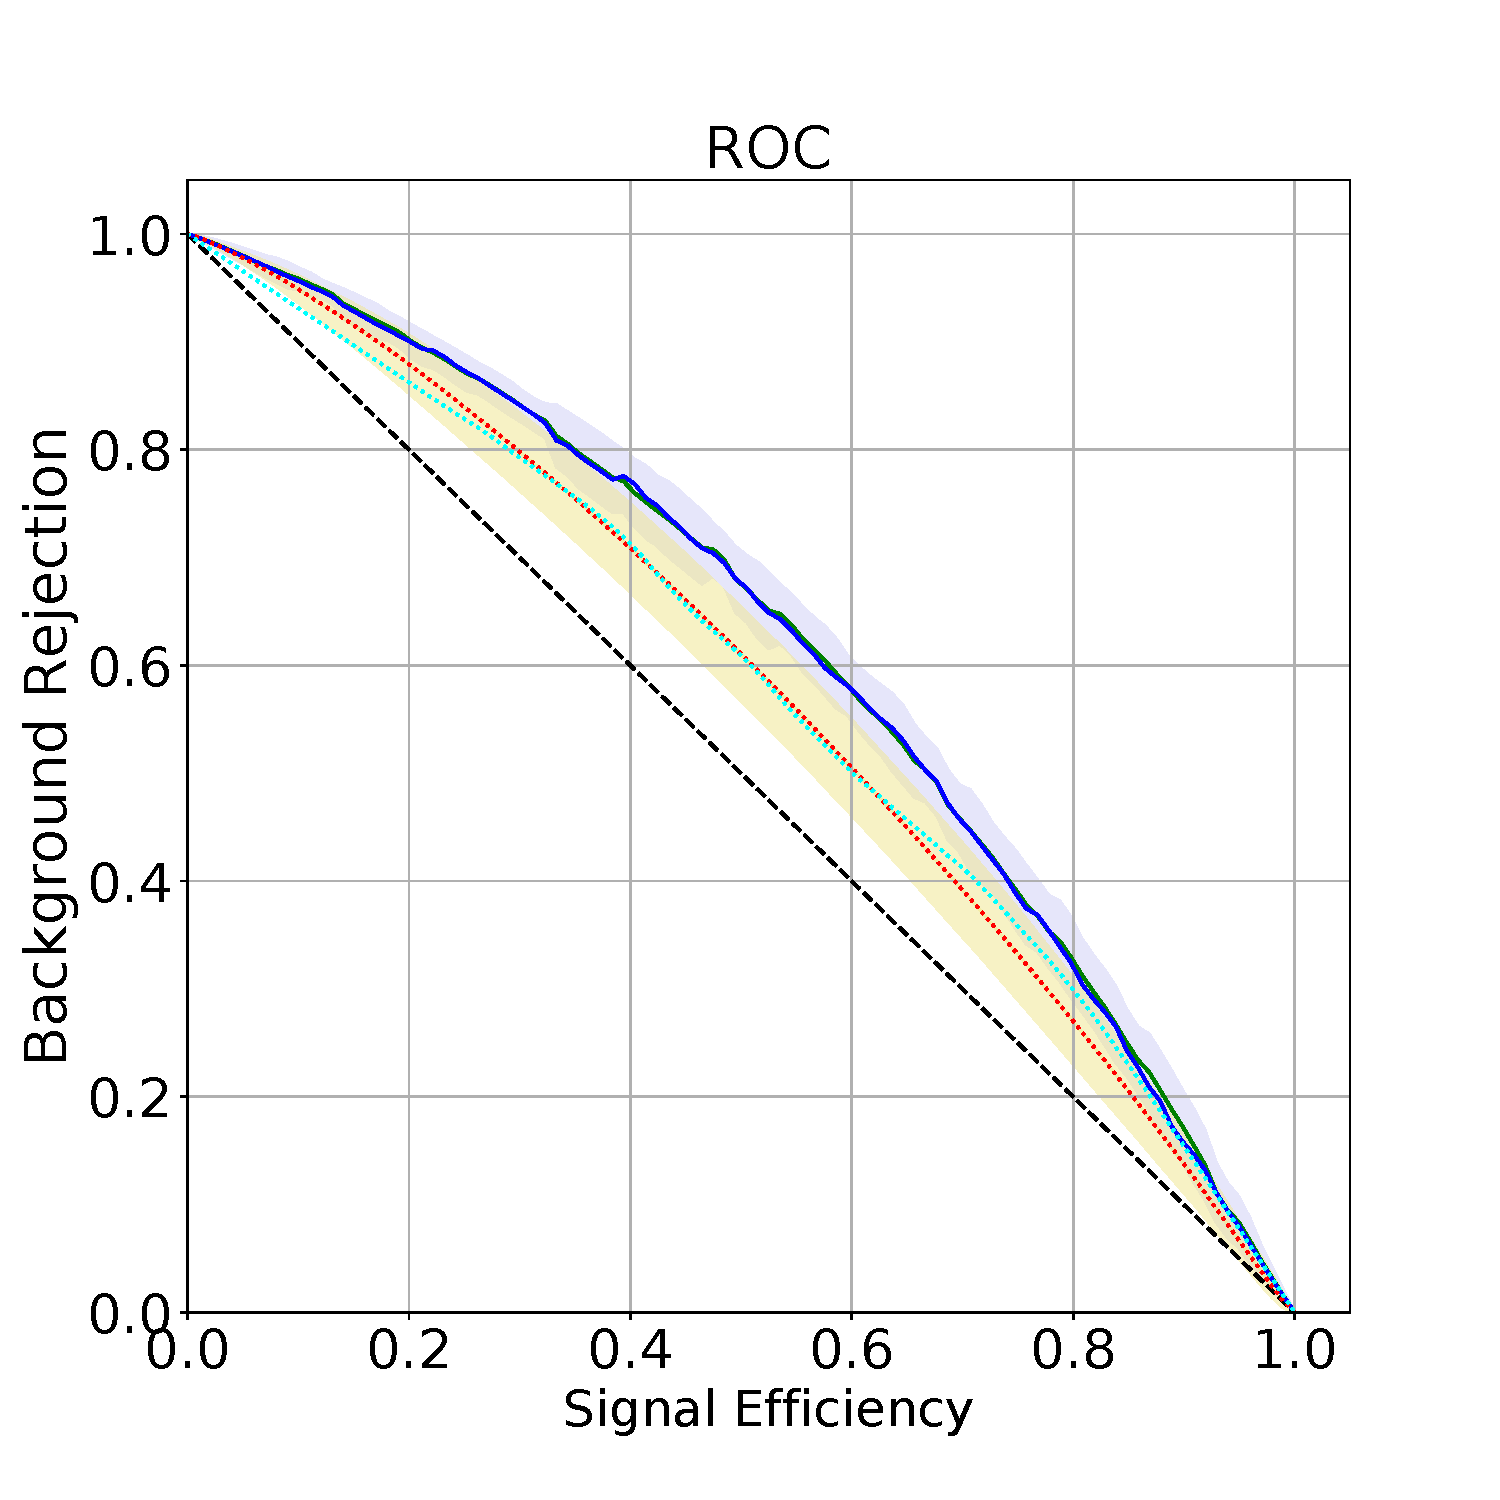
\includegraphics[width=0.5\textwidth]{Fig3b-ROC_example_100SAXGB}}\\
  \subfloat[]{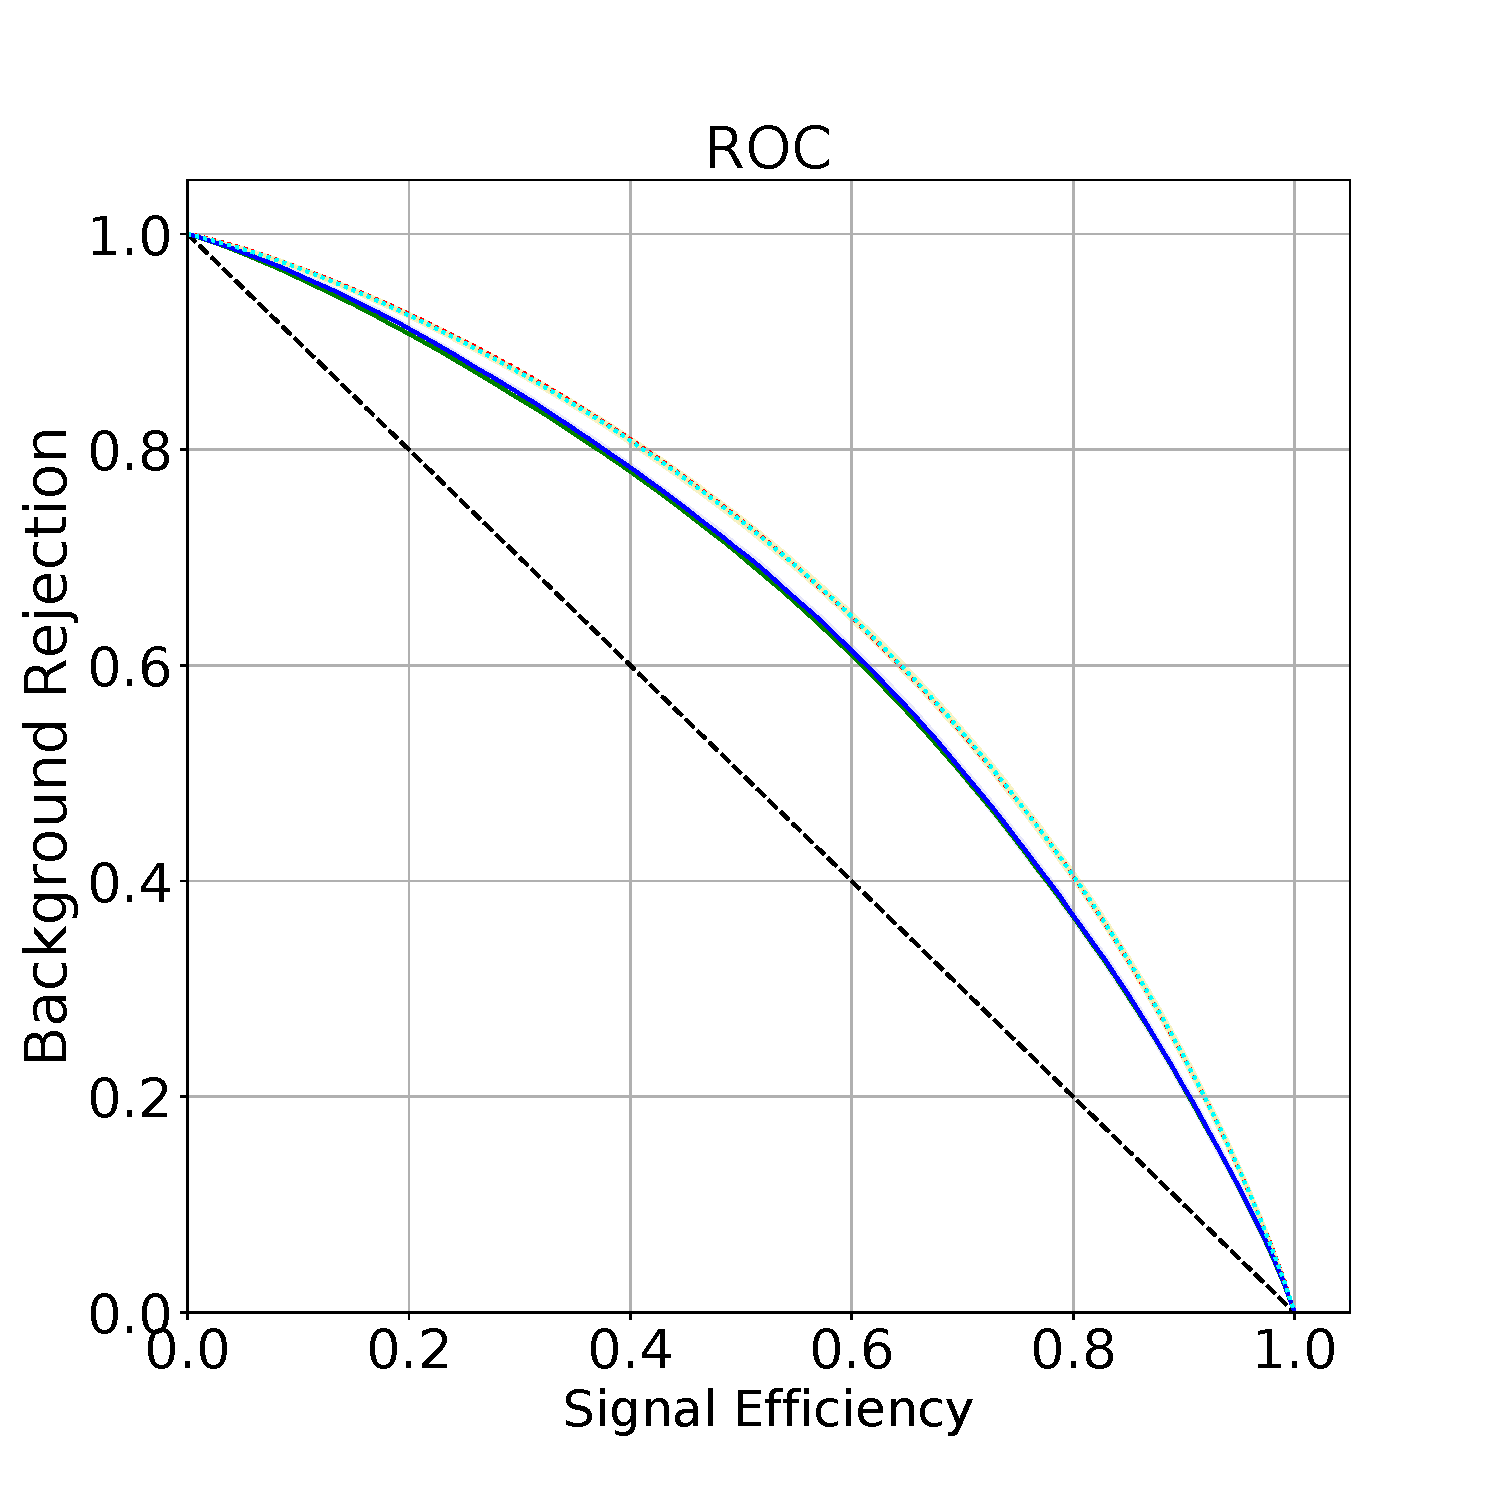
\includegraphics[width=0.5\textwidth]{Fig3c-ROC_example_20000DWDNN}}
  \subfloat[]{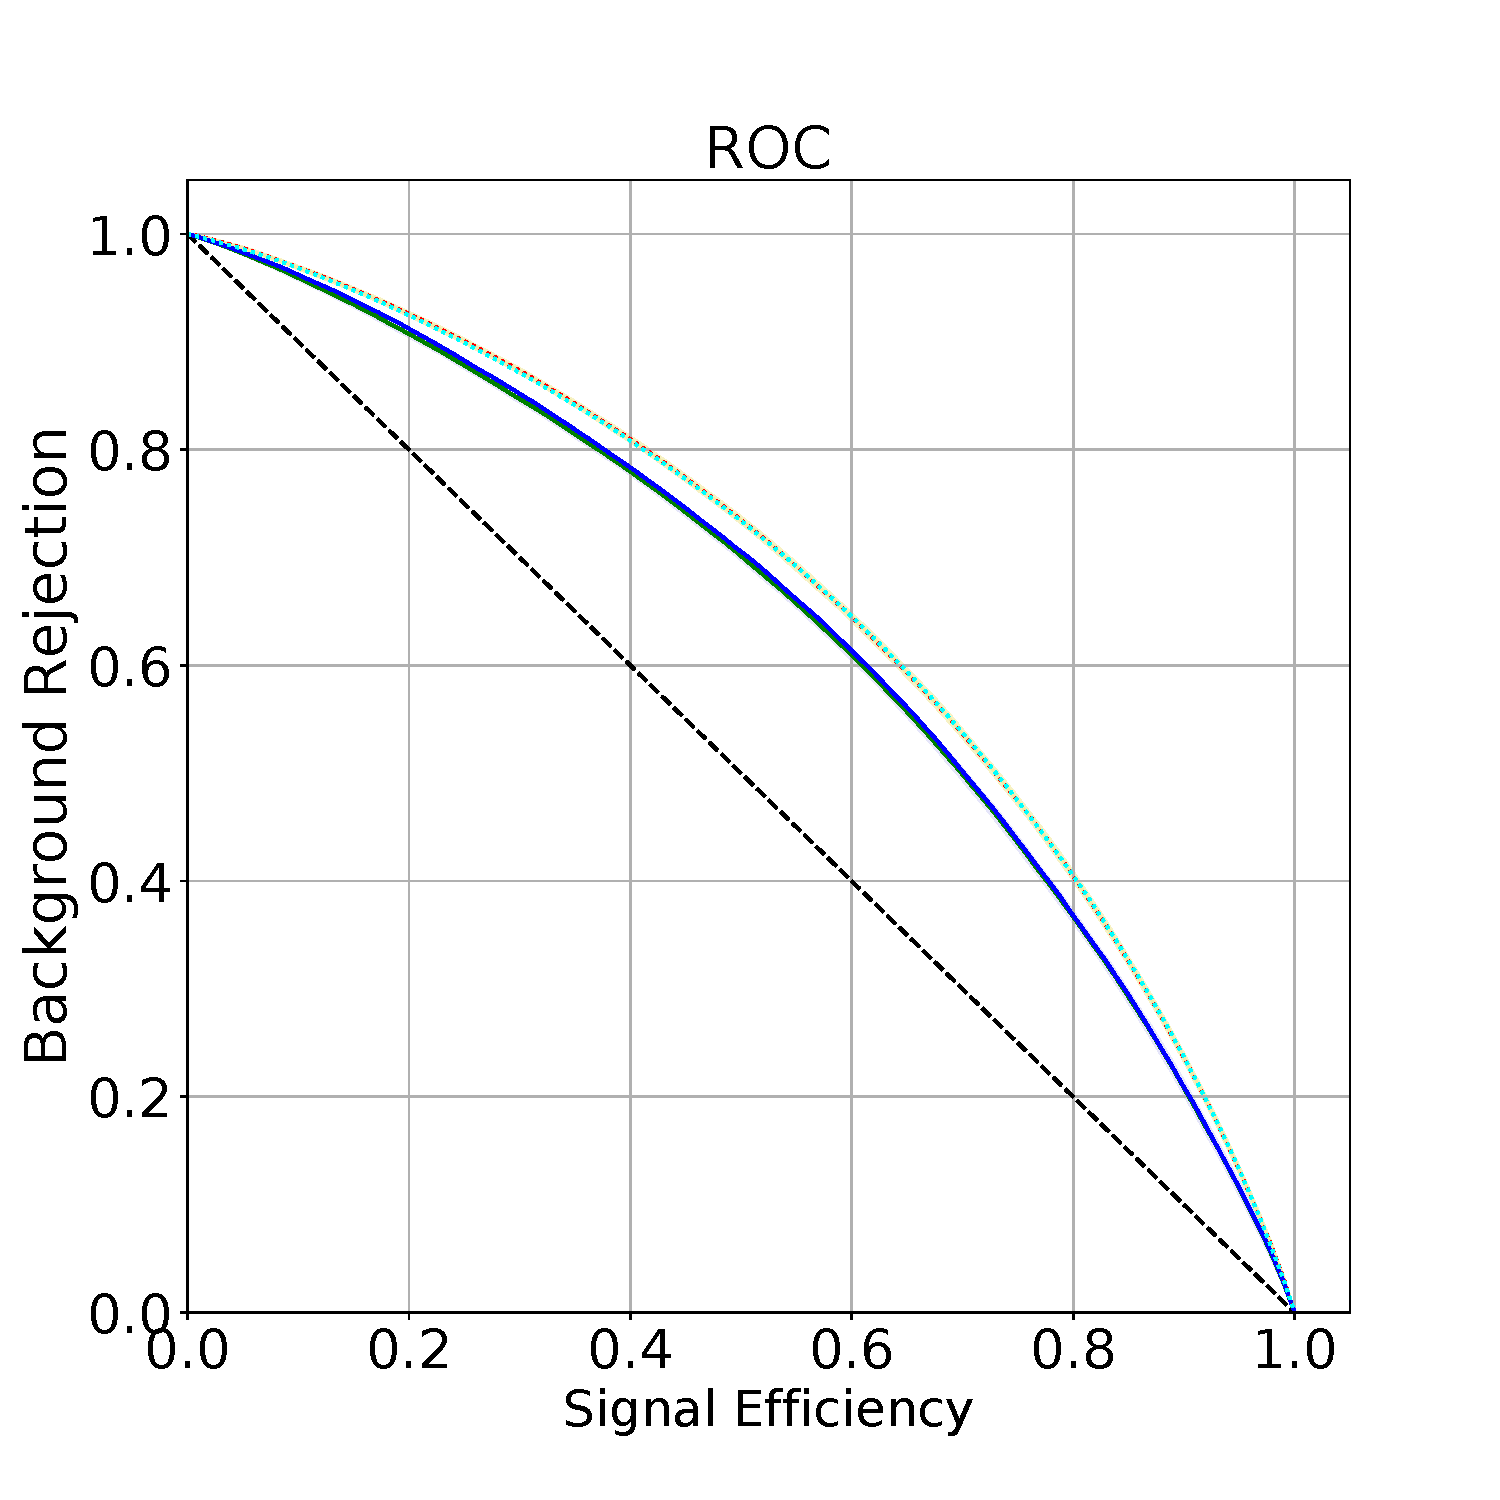
\includegraphics[width=0.5\textwidth]{Fig3d-ROC_example_20000SAXGB}}
  \caption{\textbf{ROC curves} for the annealer-trained networks (DW and SA) at $f=0.05$, DNN, and XGB. Error bars are defined by the variation over the training sets and statistical error. Both panels show all four ROC curves, with solid lines for DW (green) and SA (blue), and dotted lines for DNN (red) and XGB (cyan). Panels (a) and (c) [(b) and (d)] includes $1\sigma$ error bars only for DW and DNN [SA and XGB], in light blue and pale yellow, respectively. Results shown are for the $36$ variable networks at $\lambda=0.05$ trained on $100$ events for panels (a) and (b), and on $20,000$ events for panels (c) and (d). For $100$ events the annealer trained networks have a larger area under the ROC curve, as shown directly in Fig.~\ref{fig:aurocs}. The situation is reversed for $20,000$ training events, where the error bars are too small to be visible. The much smaller error bars are due to the increased number of events.}
 \label{fig:rocs}
 \end{figure*}


\begin{figure*}[hbt]
%\centering
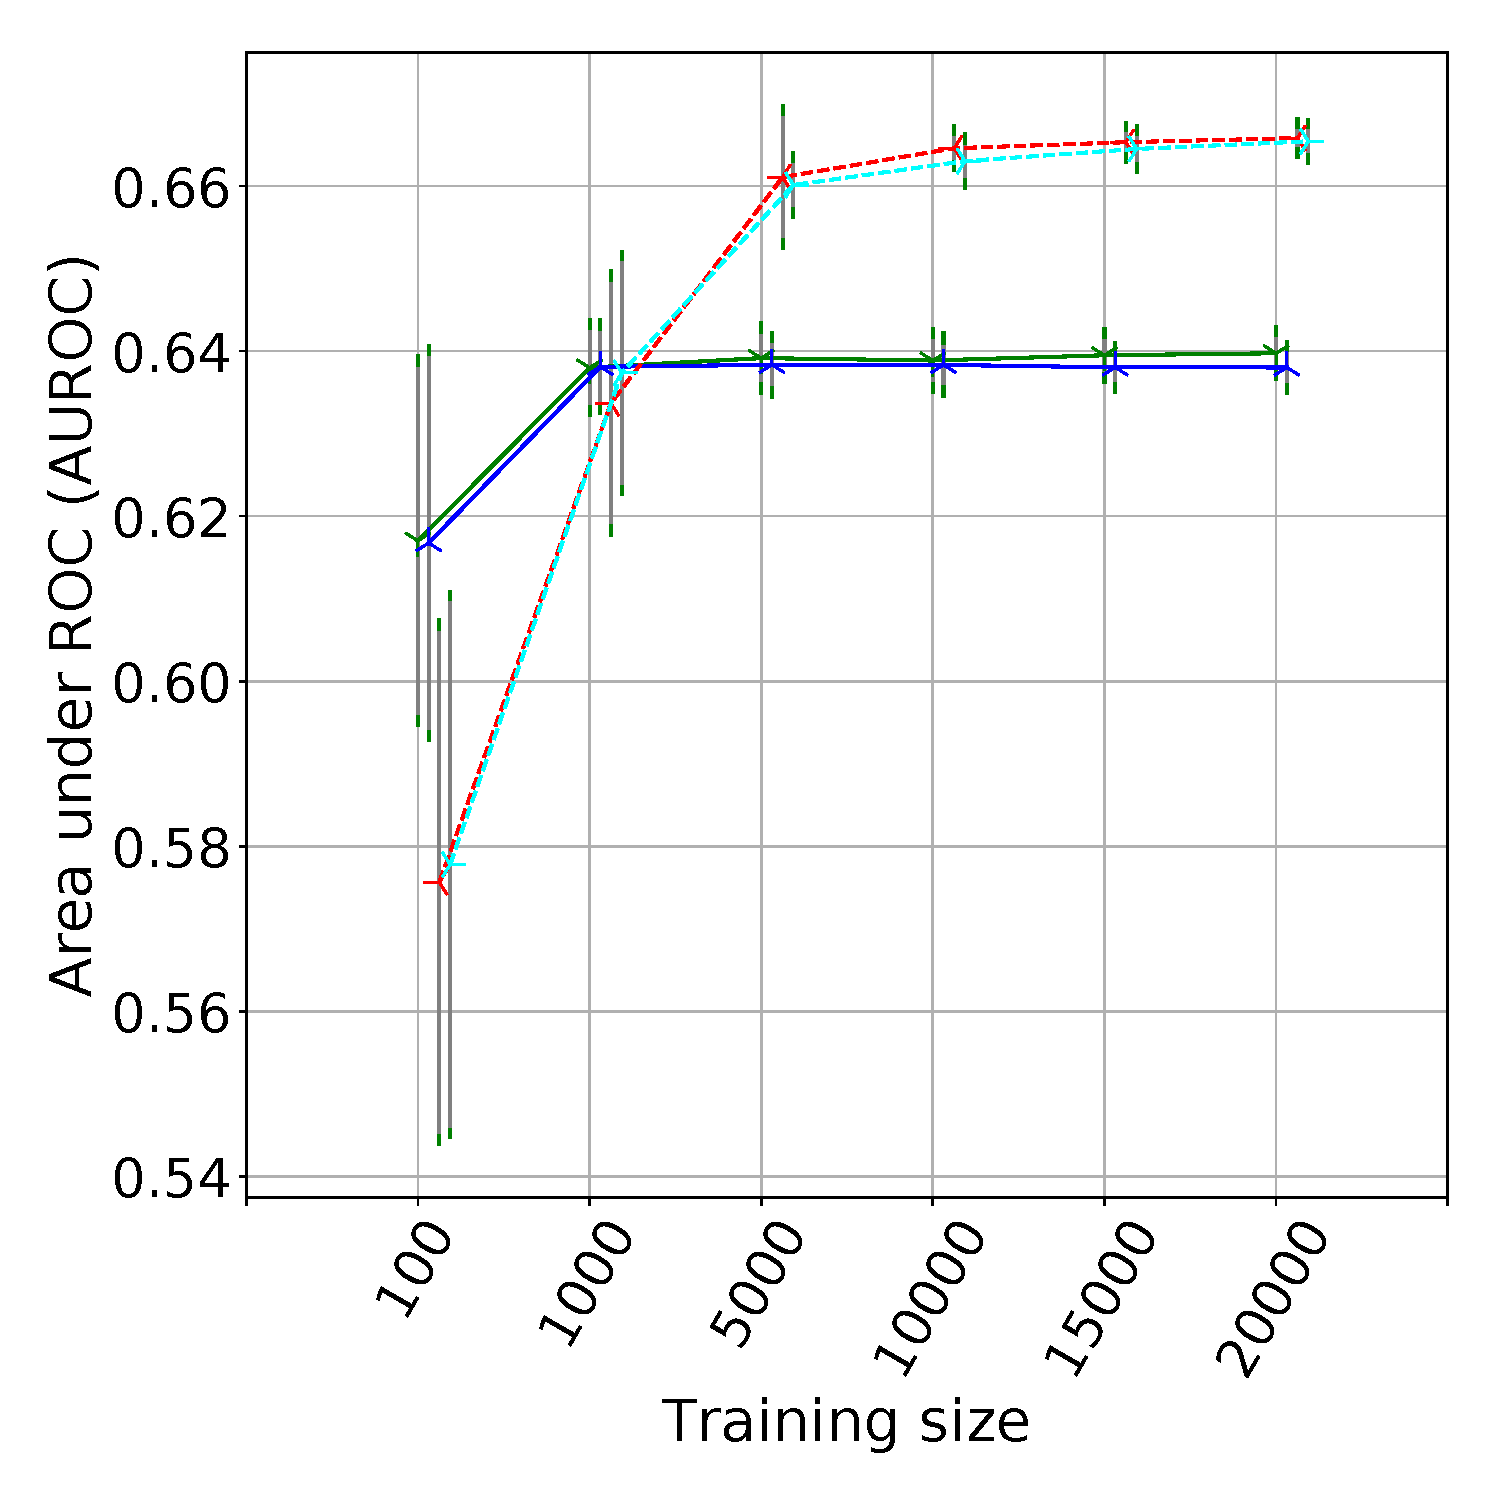
\includegraphics[width=\textwidth]{Fig4-aucs}
\caption{
\textbf{Area under the ROC curves (AUROCs)} for the annealer-trained networks (DW (green) and SA (blue), solid lines) at $f=0.05$, and the conventional approaches (DNN (red) and XGB (cyan), dotted lines).
The vertical lines denote 1$\sigma$ error bars,  defined by the variation over the training sets (grey) plus statistical error (green); see the SI (Sec.~6) for details of the uncertainty analysis. While DNN and XGB have an advantage at large training sizes, we find that the annealer-trained networks perform better for small training sizes. Results shown are for the $36$ variable networks at $\lambda=0.05$. The overall QAML performance and its features, including the advantage at small training sizes and saturation at $\approx 0.64$, are stable across a range of values for $\lambda$. An extended version of this plot with various values of $\lambda$ is available in the SI in Fig.~2.}
%\ref{fig:aucs_lambdas}
\label{fig:aurocs}
\end{figure*}

 \begin{figure*}[hbt]
  \subfloat[]{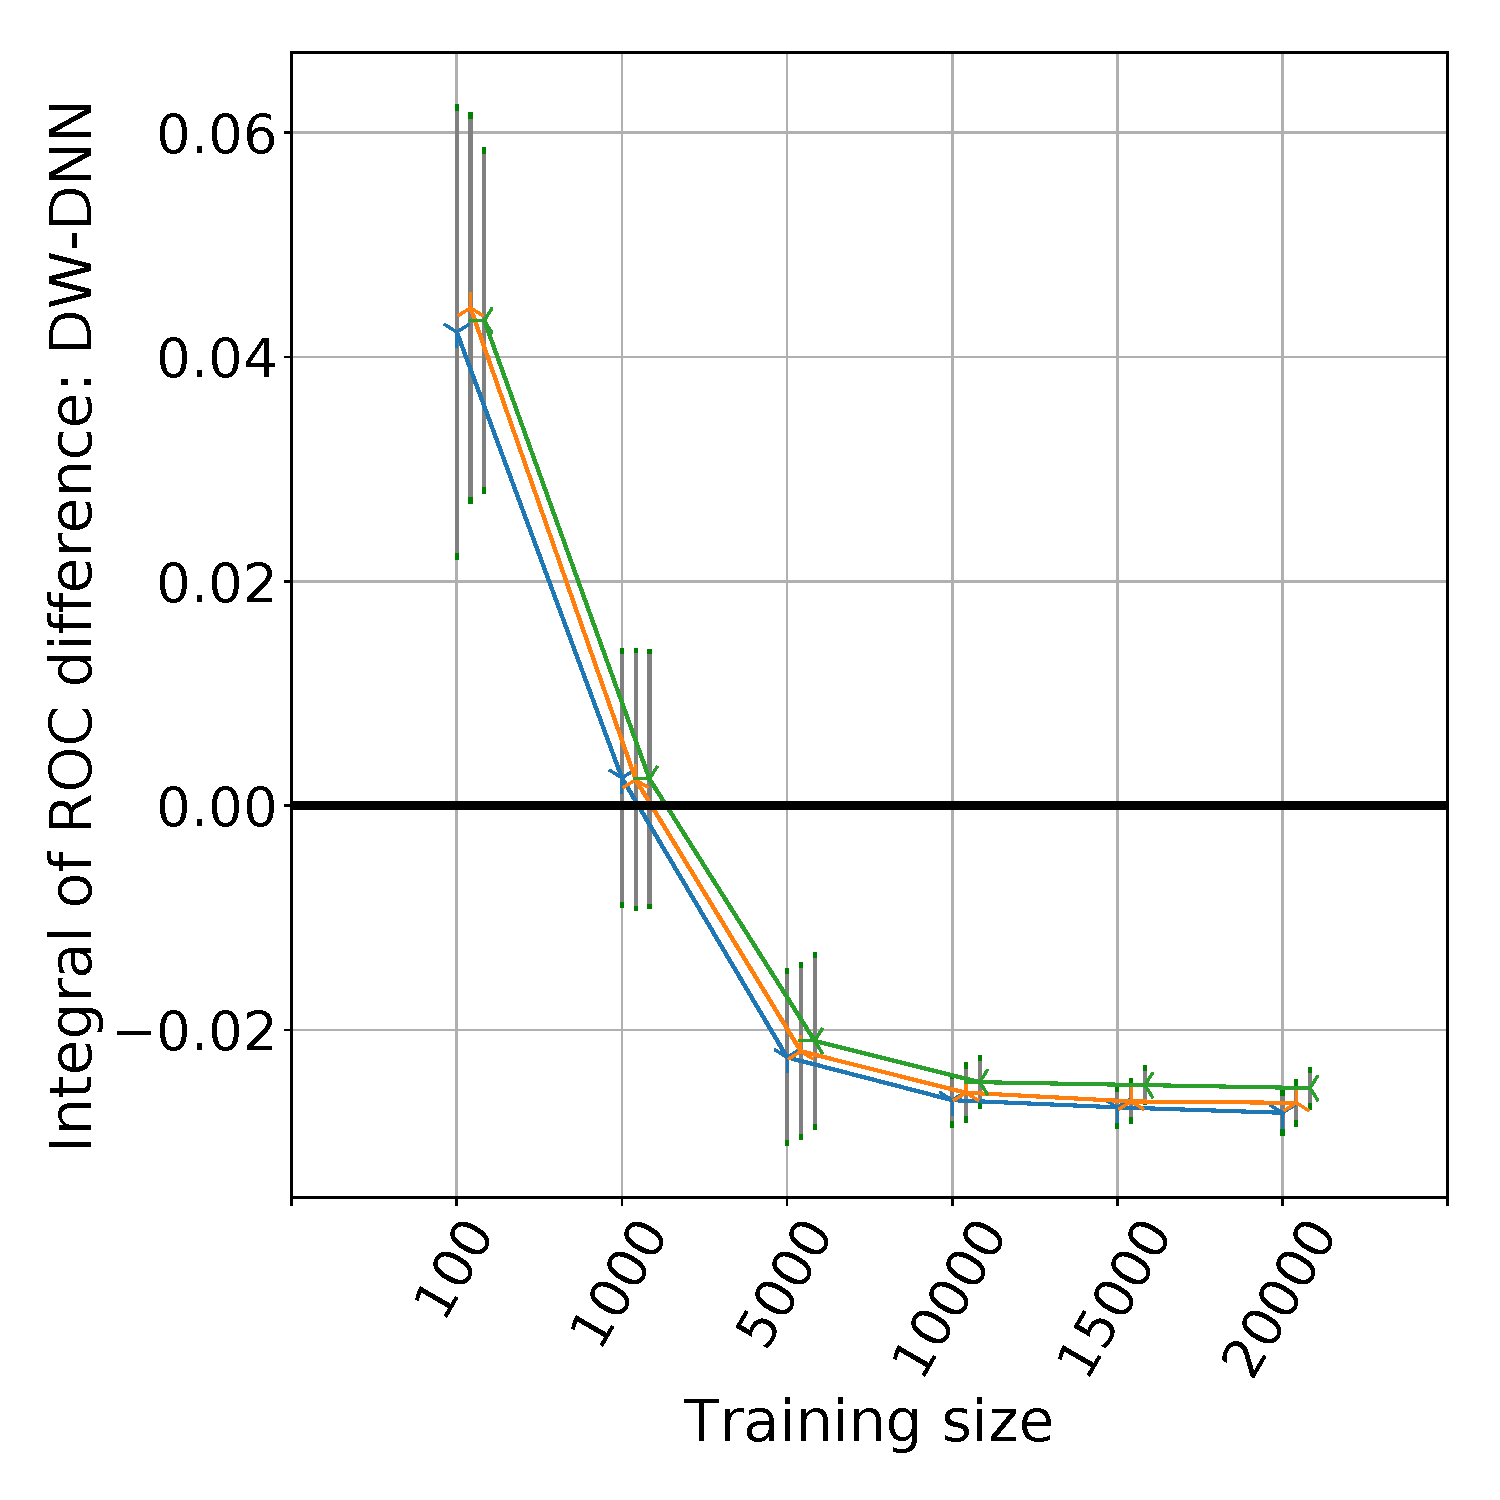
\includegraphics[width=0.34\textwidth]{Fig5a-full_DW--DNN_auc}}
  \subfloat[]{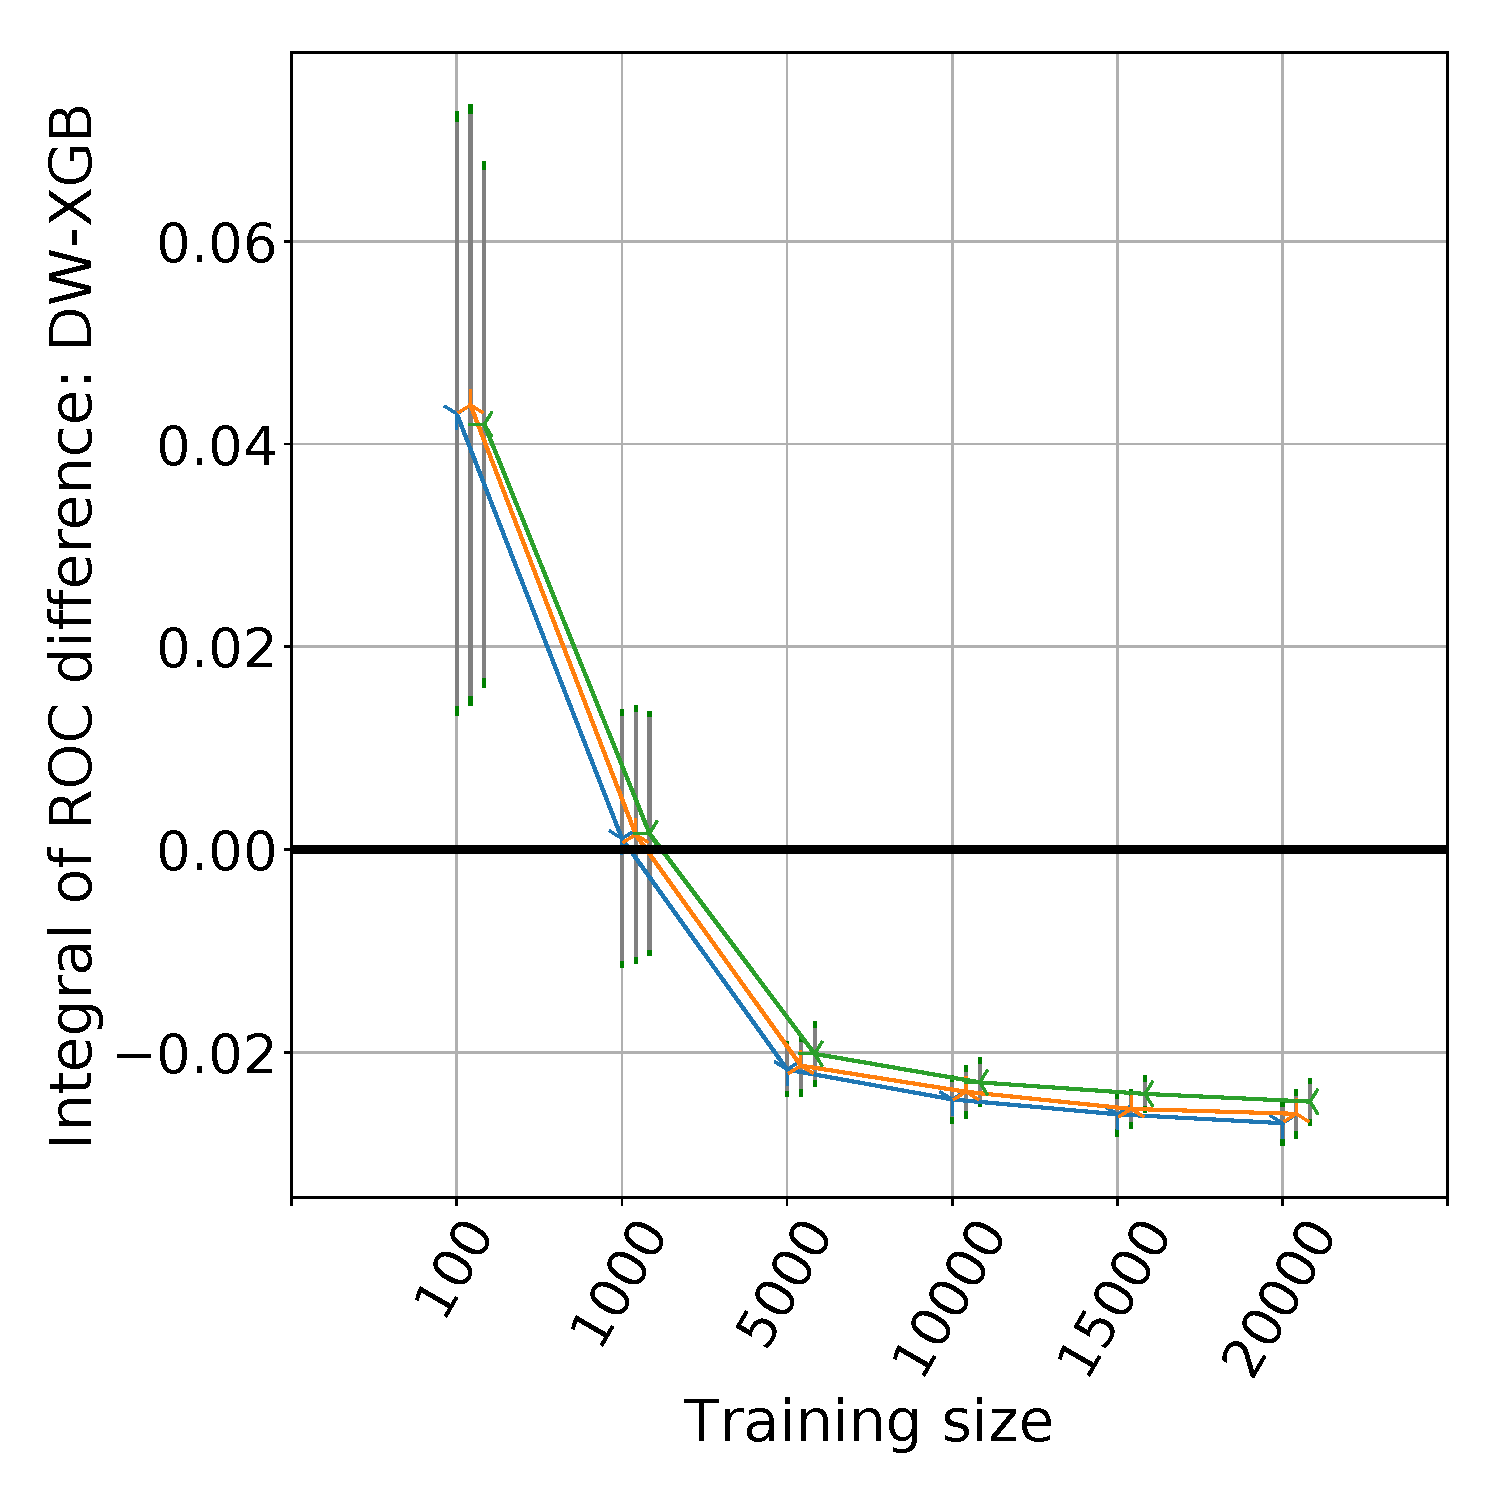
\includegraphics[width=0.34\textwidth]{Fig5b-full_DW--XGB_auc}}
  \subfloat[]{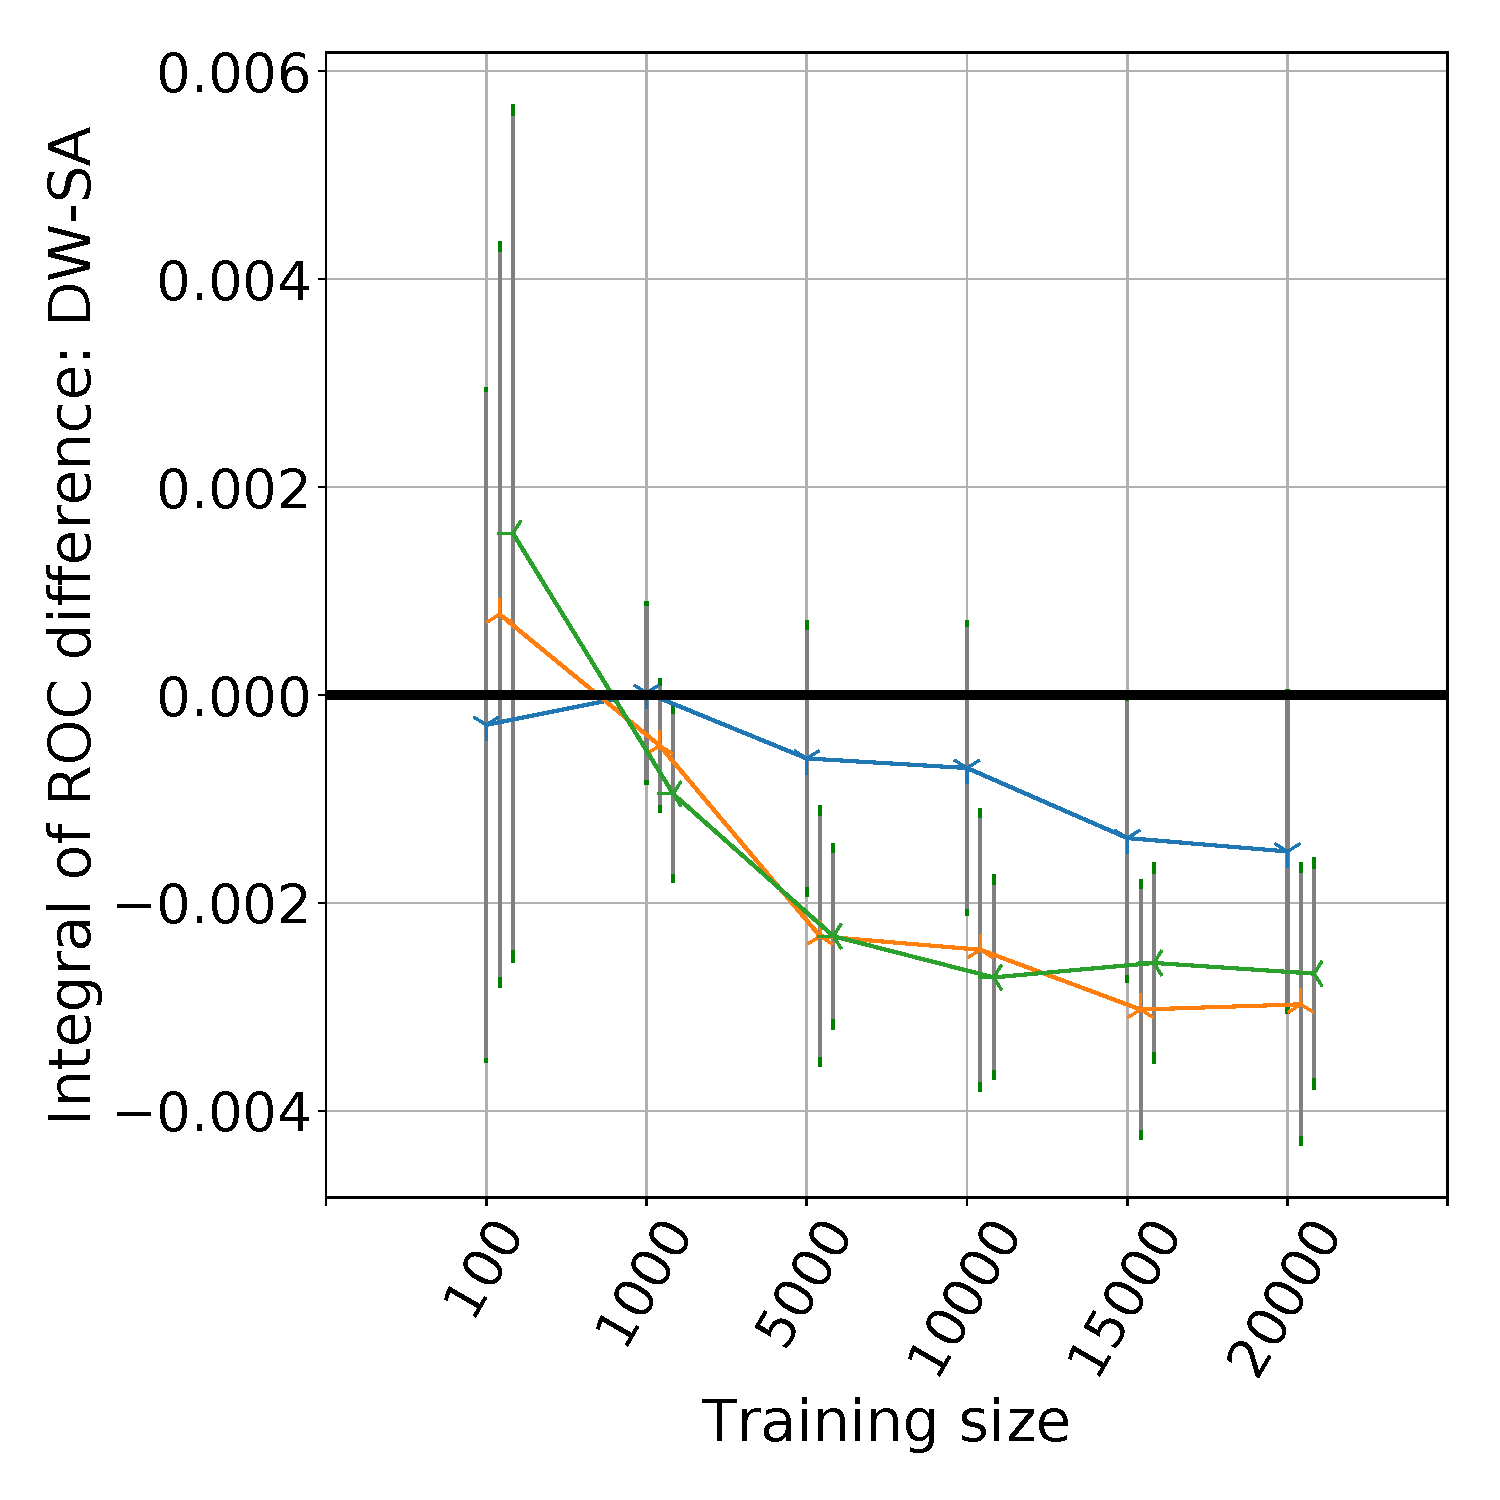
\includegraphics[width=0.34\textwidth]{Fig5c-full_DW--SA_auc}}
 \caption{\textbf{Difference between AUROCs} of (a) DW vs DNN, (b) DW vs XGBoost, and (c) DW vs SA, as a function of training size and fraction $f$ above the minimum energy returned (the same values of $f$ are used for DW and SA in (c)). Formally, we plot $\int_0^1 [r_B^{(\text{DW})}(\epsilon_S)-r_B^{(i)}(\epsilon_S)] d\epsilon_S$, where $i\in\{\text{DNN, XGBoost, SA}\}$. The vertical lines denote $1\sigma$ error bars. The large error bars are due to noise on the programmed Hamiltonian.}
 \label{fig:audrocs}
 \end{figure*}
\newpage\clearpage

\begin{table*}[hbt]
\begin{tabular}{l|l}
   \textbf{variable} & \textbf{description} \\
   \hline
    $p_T^1/m_{\gamma\gamma}$ & {\small transverse momentum of the highest $p_T$ photon divided by the invariant mass of the diphoton pair}\\
    $p_T^2/m_{\gamma\gamma}$ & {\small transverse momentum of the second-highest $p_T$ photon divided by the invariant mass of the diphoton pair}\\
    $(p_T^1+p_T^2)/m_{\gamma\gamma}$ & {\small sum of the transverse momentum of the two photons divided by their invariant mass} \\
    $(p_T^1-p_T^2)/m_{\gamma\gamma}$ & {\small difference of the transverse momentum of the two photons divided by their invariant mass} \\
    $p_T^{\gamma\gamma}/m_{\gamma\gamma}$ & {\small transverse momentum of the diphoton system divided by its invariant mass} \\
    $\Delta\eta$ & {\small difference in $\eta=-\log\tan(\frac{\theta}{2})$, where $\theta$ is the angle with the beam axis} \\
    $\Delta R$ & {\small sum in quadrature of the separation of and $\phi$, the azimuthal angle of the two photons $(\sqrt{\Delta\eta^2+\Delta\phi^2})$} \\
    $\abs{\eta^{\gamma\gamma}}$ & {\small the $\eta$ value of the diphoton system}
  \end{tabular}
  \caption{\textbf{The kinematical variables used to construct weak classifiers.}}
  \label{tab:kinematic_variables}
 \end{table*}
 \newpage\clearpage
 %\begin{figure*}[hbt]	
%\end{figure*}

% Please add the following required packages to your document preamble:
% \usepackage[table,xcdraw]{xcolor}
% If you use beamer only pass "xcolor=table" option, i.e. \documentclass[xcolor=table]{beamer}
% Please add the following required packages to your document preamble:
% \usepackage[table,xcdraw]{xcolor}
% If you use beamer only pass "xcolor=table" option, i.e. \documentclass[xcolor=table]{beamer}
\begin{table}[]
\centering
\caption{\textbf{Map from number to variable/weak-classifier name}}
\label{tab:kinematic_variables_key}
\begin{tabular}{|l|l|l|l|l|l|l|l|l|}
\hline
\cellcolor[HTML]{34FF34} 1                                      & \cellcolor[HTML]{34FF34} 2                             & \cellcolor[HTML]{34FF34} 3                                           & \cellcolor[HTML]{34FF34} 4                                                   & \cellcolor[HTML]{34FF34} 5                                         &  \cellcolor[HTML]{34FF34}6                                          & \cellcolor[HTML]{34FF34} 7                                       & \cellcolor[HTML]{34FF34} 8                                          & \cellcolor[HTML]{34FF34} 9                                             \\\hline
$ p_T^1 $                              & $ p_T^2 $                     & $ \Delta R $                                & $ p_T^{\gamma\gamma} $                              & $ p_T^1+p_T^2 $                           & $ p_T^1-p_T^2 $                            & $ \Delta\eta $                          & $ \eta_{\gamma\gamma} $                    & $ (p_T^1+p_T^2) \eta_{\gamma\gamma} $         \\\hline
\cellcolor[HTML]{34FF34} 10                                     & \cellcolor[HTML]{34FF34}11                            & \cellcolor[HTML]{34FF34}12                                          & \cellcolor[HTML]{34FF34}13                                                  & \cellcolor[HTML]{34FF34}14                                        & \cellcolor[HTML]{34FF34}15                                         & \cellcolor[HTML]{34FF34}16                                      & \cellcolor[HTML]{34FF34}17                                         & \cellcolor[HTML]{34FF34}18                                            \\\hline
$\frac{ p_T^2}{ p_T^1-p_T^2} $         & $ \frac{p_T^2}{ \Delta\eta} $ & $ p_T^2 \eta_{\gamma\gamma} $               & $\frac{1}{\Delta R  p_T^{\gamma\gamma}}$              & $ \frac{p_T^1+p_T^2}{ \Delta R} $         & $\frac{1}{\Delta R  ( p_T^1-p_T^2)}$         & $ \frac{1}{\Delta R \Delta\eta} $          & $\frac{ \eta_{\gamma\gamma} }{ \Delta R }$ & $\frac{1}{(p_T^1-p_T^2) \Delta\eta} $            \\\hline
\cellcolor[HTML]{34FF34}19                                     & \cellcolor[HTML]{34FF34}20                            & \cellcolor[HTML]{34FF34}21                                          & \cellcolor[HTML]{34FF34}22                                                  & \cellcolor[HTML]{34FF34}23                                        & \cellcolor[HTML]{34FF34}24                                         & \cellcolor[HTML]{34FF34}25                                      & \cellcolor[HTML]{34FF34}26                                         &\cellcolor[HTML]{34FF34} 27                                            \\\hline
$ p_T^1 p_T^2 $                        & $ \frac{p_T^1 }{ \Delta R }$  & $ \frac{p_T^1}{ p_T^{\gamma\gamma}} $       & $ p_T^1  (p_T^1+p_T^2) $                            & $\frac{ p_T^1}{ p_T^1-p_T^2} $            & $ \frac{p_T^1 }{ \Delta\eta} $             & $\frac{ p_T^1 }{ \eta_{\gamma\gamma}} $ & $\frac{ p_T^2 }{\Delta R} $                & $ \frac{\eta_{\gamma\gamma} }{ p_T^1-p_T^2 }$ \\\hline
\cellcolor[HTML]{34FF34}28                                     & \cellcolor[HTML]{34FF34}29                            & \cellcolor[HTML]{34FF34}30                                          & \cellcolor[HTML]{34FF34}31                                                  & \cellcolor[HTML]{34FF34}32                                        & \cellcolor[HTML]{34FF34}33                                         & \cellcolor[HTML]{34FF34}34                                      & \cellcolor[HTML]{34FF34}35                                         & \cellcolor[HTML]{34FF34}36                                            \\\hline
$\frac{ p_T^2 }{ p_T^{\gamma\gamma}} $ & $ p_T^2 (p_T^1+p_T^2) $       & $ \frac{p_T^1+p_T^2}{ p_T^{\gamma\gamma} }$ & $\frac{ \eta_{\gamma\gamma}}{ p_T^{\gamma\gamma}} $ & $ \frac{1}{p_T^{\gamma\gamma}  \Delta\eta} $ & $\frac{1}{p_T^{\gamma\gamma} (p_T^1-p_T^2)} $ & $ \frac{p_T^1+p_T^2 }{ p_T^1-p_T^2 }$   & $\frac{ p_T^1+p_T^2 }{ \Delta\eta} $       & $\frac{ \eta_{\gamma\gamma} }{\Delta\eta} $  \\\hline
\end{tabular}
\end{table}
\newpage\clearpage
\begin{table}[]
\centering
\caption{\textbf{Variable inclusion in the ground states of the Ising problem instances}. The variables listed are those from which we selected the various variables included in our tests with varying problem size. We list how many out of $20$ training sets had the given variable turned on in the ground state configuration. Three of the $36$ variables were included for all values of the penalty term $\lambda$ and for all of the training sets [$ p_T^2 $, $(\Delta R  p_T^{\gamma\gamma} )^{-1}$, and $\frac{ p_T^2 }{ p_T^{\gamma\gamma}} $], the variables $p_T^2/(p_T^1-p_T^2)$ and $(p_T^1+p_T^2)/\Delta\eta$ were present in almost all, while seven were never included, among which the original kinematical variables $ p_T^1 $ and $ \eta_{\gamma\gamma}$. All momenta ($p_T^1,p_T^2,p_T^{\gamma\gamma}$) are given in units of $m_{\gamma\gamma}$.
Variables are given in Table~\ref{tab:kinematic_variables_key}.}
  \label{fig:variableinclusion}
\label{my-label}
\begin{tabular}{l|llllllllllllllllll}
$\lambda$ & 1                                                & 2                          & 3                          & 4                          & 5                          & 6                          & 7                          & 8                         & 9                         & 10                         & 11                         & 12                         & 13                         & 14                         & 15                         & 16                         & 17                         & 18                                                \\ \hline
0      & \cellcolor[HTML]{FE0000}{\color[HTML]{333333} 0} & \cellcolor[HTML]{34FF34}20 & \cellcolor[HTML]{34FF34}20 & \cellcolor[HTML]{34FF34}20 & \cellcolor[HTML]{ABFF34}19 & \cellcolor[HTML]{34FF34}20 & \cellcolor[HTML]{34FF34}20 & \cellcolor[HTML]{FE0000}0 & \cellcolor[HTML]{FEA800}5 & \cellcolor[HTML]{34FF34}20 & \cellcolor[HTML]{34FF34}20 & \cellcolor[HTML]{34FF34}20 & \cellcolor[HTML]{34FF34}20 & \cellcolor[HTML]{ABFF34}19 & \cellcolor[HTML]{34FF34}20 & \cellcolor[HTML]{ABFF34}17 & \cellcolor[HTML]{34FF34}20 & \cellcolor[HTML]{34FF34}{\color[HTML]{000000} 20} \\
0.01   & \cellcolor[HTML]{FE0000}{\color[HTML]{333333} 0} & \cellcolor[HTML]{34FF34}20 & \cellcolor[HTML]{34FF34}20 & \cellcolor[HTML]{34FF34}20 & \cellcolor[HTML]{ABFF34}19 & \cellcolor[HTML]{34FF34}20 & \cellcolor[HTML]{34FF34}20 & \cellcolor[HTML]{FE0000}0 & \cellcolor[HTML]{FE9D00}4 & \cellcolor[HTML]{34FF34}20 & \cellcolor[HTML]{34FF34}20 & \cellcolor[HTML]{34FF34}20 & \cellcolor[HTML]{34FF34}20 & \cellcolor[HTML]{ABFF34}19 & \cellcolor[HTML]{34FF34}20 & \cellcolor[HTML]{ABFF34}17 & \cellcolor[HTML]{34FF34}20 & \cellcolor[HTML]{34FF34}{\color[HTML]{000000} 20} \\
0.02   & \cellcolor[HTML]{FE0000}{\color[HTML]{333333} 0} & \cellcolor[HTML]{34FF34}20 & \cellcolor[HTML]{34FF34}20 & \cellcolor[HTML]{34FF34}20 & \cellcolor[HTML]{ABFF34}19 & \cellcolor[HTML]{34FF34}20 & \cellcolor[HTML]{34FF34}20 & \cellcolor[HTML]{FE0000}0 & \cellcolor[HTML]{FE9D00}4 & \cellcolor[HTML]{34FF34}20 & \cellcolor[HTML]{34FF34}20 & \cellcolor[HTML]{34FF34}20 & \cellcolor[HTML]{34FF34}20 & \cellcolor[HTML]{ABFF34}19 & \cellcolor[HTML]{34FF34}20 & \cellcolor[HTML]{BDFF34}16 & \cellcolor[HTML]{34FF34}20 & \cellcolor[HTML]{34FF34}{\color[HTML]{000000} 20} \\
0.05   & \cellcolor[HTML]{FE0000}{\color[HTML]{333333} 0} & \cellcolor[HTML]{34FF34}20 & \cellcolor[HTML]{34FF34}20 & \cellcolor[HTML]{34FF34}20 & \cellcolor[HTML]{ABFF34}19 & \cellcolor[HTML]{34FF34}20 & \cellcolor[HTML]{34FF34}20 & \cellcolor[HTML]{FE0000}0 & \cellcolor[HTML]{FE5A00}1 & \cellcolor[HTML]{34FF34}20 & \cellcolor[HTML]{34FF34}20 & \cellcolor[HTML]{34FF34}20 & \cellcolor[HTML]{34FF34}20 & \cellcolor[HTML]{ABFF34}19 & \cellcolor[HTML]{34FF34}20 & \cellcolor[HTML]{F8FF00}10 & \cellcolor[HTML]{34FF34}20 & \cellcolor[HTML]{ABFF34}17                        \\
0.1    & \cellcolor[HTML]{FE0000}{\color[HTML]{333333} 0} & \cellcolor[HTML]{34FF34}20 & \cellcolor[HTML]{34FF34}20 & \cellcolor[HTML]{34FF34}20 & \cellcolor[HTML]{ABFF34}19 & \cellcolor[HTML]{34FF34}20 & \cellcolor[HTML]{34FF34}20 & \cellcolor[HTML]{FE0000}0 & \cellcolor[HTML]{FE0000}0 & \cellcolor[HTML]{34FF34}20 & \cellcolor[HTML]{34FF34}20 & \cellcolor[HTML]{34FF34}20 & \cellcolor[HTML]{34FF34}20 & \cellcolor[HTML]{ABFF34}19 & \cellcolor[HTML]{34FF34}20 & \cellcolor[HTML]{FEA800}6  & \cellcolor[HTML]{CFFF34}14 & \cellcolor[HTML]{FE5A00}2                         \\
0.2    & \cellcolor[HTML]{FE0000}{\color[HTML]{333333} 0} & \cellcolor[HTML]{34FF34}20 & \cellcolor[HTML]{34FF34}20 & \cellcolor[HTML]{34FF34}20 & \cellcolor[HTML]{ABFF34}19 & \cellcolor[HTML]{34FF34}20 & \cellcolor[HTML]{34FF34}20 & \cellcolor[HTML]{FE0000}0 & \cellcolor[HTML]{FE0000}0 & \cellcolor[HTML]{34FF34}20 & \cellcolor[HTML]{CFFF34}14 & \cellcolor[HTML]{34FF34}20 & \cellcolor[HTML]{34FF34}20 & \cellcolor[HTML]{EFFE00}12 & \cellcolor[HTML]{34FF34}20 & \cellcolor[HTML]{FE9D00}4  & \cellcolor[HTML]{FE4300}1  & \cellcolor[HTML]{FE0000}0                         \\
0.4    & \cellcolor[HTML]{FE0000}{\color[HTML]{333333} 0} & \cellcolor[HTML]{34FF34}20 & \cellcolor[HTML]{FE0000}0  & \cellcolor[HTML]{FE5A00}2  & \cellcolor[HTML]{ABFF34}19 & \cellcolor[HTML]{34FF34}20 & \cellcolor[HTML]{34FF34}20 & \cellcolor[HTML]{FE0000}0 & \cellcolor[HTML]{FE0000}0 & \cellcolor[HTML]{34FF34}20 & \cellcolor[HTML]{ABFF34}17 & \cellcolor[HTML]{34FF34}20 & \cellcolor[HTML]{34FF34}20 & \cellcolor[HTML]{FE0000}0  & \cellcolor[HTML]{34FF34}20 & \cellcolor[HTML]{FE4300}1  & \cellcolor[HTML]{FE0000}0  & \cellcolor[HTML]{FE0000}0                         \\
0.8    & \cellcolor[HTML]{FE0000}{\color[HTML]{333333} 0} & \cellcolor[HTML]{34FF34}20 & \cellcolor[HTML]{FE0000}0  & \cellcolor[HTML]{FE0000}0  & \cellcolor[HTML]{FE0000}0  & \cellcolor[HTML]{FE0000}0  & \cellcolor[HTML]{FEF600}9  & \cellcolor[HTML]{FE0000}0 & \cellcolor[HTML]{FE0000}0 & \cellcolor[HTML]{ABFF34}18 & \cellcolor[HTML]{FE0000}0  & \cellcolor[HTML]{FE0000}0  & \cellcolor[HTML]{34FF34}20 & \cellcolor[HTML]{FE0000}0  & \cellcolor[HTML]{FE5A00}2  & \cellcolor[HTML]{FE0000}0  & \cellcolor[HTML]{FE0000}0  & \cellcolor[HTML]{FE0000}0  \\
\\                      
$\lambda$ & 19                         & 20                        & 21                        & 22                         & 23                        & 24                         & 25                        & 26                        & 27                        & 28                         & 29                         & 30                        & 31                        & 32                         & 33                        & 34                         & 35                         & 36                         \\\hline
0      & \cellcolor[HTML]{34FF34}20 & \cellcolor[HTML]{FE0000}0 & \cellcolor[HTML]{FE0000}0 & \cellcolor[HTML]{ABFF34}19 & \cellcolor[HTML]{FE0000}0 & \cellcolor[HTML]{34FF34}20 & \cellcolor[HTML]{FE0000}0 & \cellcolor[HTML]{FE7000}3 & \cellcolor[HTML]{FE0000}0 & \cellcolor[HTML]{34FF34}20 & \cellcolor[HTML]{ABFF34}19 & \cellcolor[HTML]{FEA800}7 & \cellcolor[HTML]{FE0000}0 & \cellcolor[HTML]{BDFF34}15 & \cellcolor[HTML]{FE0000}0 & \cellcolor[HTML]{ABFF34}19 & \cellcolor[HTML]{34FF34}20 & \cellcolor[HTML]{34FF34}20 \\
0.01   & \cellcolor[HTML]{34FF34}20 & \cellcolor[HTML]{FE0000}0 & \cellcolor[HTML]{FE0000}0 & \cellcolor[HTML]{ABFF34}19 & \cellcolor[HTML]{FE0000}0 & \cellcolor[HTML]{34FF34}20 & \cellcolor[HTML]{FE0000}0 & \cellcolor[HTML]{FE5A00}2 & \cellcolor[HTML]{FE0000}0 & \cellcolor[HTML]{34FF34}20 & \cellcolor[HTML]{ABFF34}19 & \cellcolor[HTML]{FE9200}6 & \cellcolor[HTML]{FE0000}0 & \cellcolor[HTML]{BDFF34}15 & \cellcolor[HTML]{FE0000}0 & \cellcolor[HTML]{ABFF34}19 & \cellcolor[HTML]{34FF34}20 & \cellcolor[HTML]{34FF34}20 \\
0.02   & \cellcolor[HTML]{34FF34}20 & \cellcolor[HTML]{FE0000}0 & \cellcolor[HTML]{FE0000}0 & \cellcolor[HTML]{ABFF34}19 & \cellcolor[HTML]{FE0000}0 & \cellcolor[HTML]{34FF34}20 & \cellcolor[HTML]{FE0000}0 & \cellcolor[HTML]{FE4300}1 & \cellcolor[HTML]{FE0000}0 & \cellcolor[HTML]{34FF34}20 & \cellcolor[HTML]{ABFF34}19 & \cellcolor[HTML]{FE8600}4 & \cellcolor[HTML]{FE0000}0 & \cellcolor[HTML]{BDFF34}15 & \cellcolor[HTML]{FE0000}0 & \cellcolor[HTML]{ABFF34}19 & \cellcolor[HTML]{34FF34}20 & \cellcolor[HTML]{34FF34}20 \\
0.05   & \cellcolor[HTML]{34FF34}20 & \cellcolor[HTML]{FE0000}0 & \cellcolor[HTML]{FE0000}0 & \cellcolor[HTML]{ABFF34}19 & \cellcolor[HTML]{FE0000}0 & \cellcolor[HTML]{34FF34}20 & \cellcolor[HTML]{FE0000}0 & \cellcolor[HTML]{FE0000}0 & \cellcolor[HTML]{FE0000}0 & \cellcolor[HTML]{34FF34}20 & \cellcolor[HTML]{BDFF34}16 & \cellcolor[HTML]{FE4300}1 & \cellcolor[HTML]{FE0000}0 & \cellcolor[HTML]{EFFE00}11 & \cellcolor[HTML]{FE0000}0 & \cellcolor[HTML]{ABFF34}19 & \cellcolor[HTML]{34FF34}20 & \cellcolor[HTML]{34FF34}20 \\
0.1    & \cellcolor[HTML]{34FF34}20 & \cellcolor[HTML]{FE0000}0 & \cellcolor[HTML]{FE0000}0 & \cellcolor[HTML]{FE4300}1  & \cellcolor[HTML]{FE0000}0 & \cellcolor[HTML]{34FF34}20 & \cellcolor[HTML]{FE0000}0 & \cellcolor[HTML]{FE0000}0 & \cellcolor[HTML]{FE0000}0 & \cellcolor[HTML]{34FF34}20 & \cellcolor[HTML]{FE4300}1  & \cellcolor[HTML]{FE0000}0 & \cellcolor[HTML]{FE0000}0 & \cellcolor[HTML]{FEA800}5  & \cellcolor[HTML]{FE0000}0 & \cellcolor[HTML]{BDFF34}16 & \cellcolor[HTML]{34FF34}20 & \cellcolor[HTML]{34FF34}20 \\
0.2    & \cellcolor[HTML]{ABFF34}18 & \cellcolor[HTML]{FE0000}0 & \cellcolor[HTML]{FE0000}0 & \cellcolor[HTML]{FE0000}0  & \cellcolor[HTML]{FE0000}0 & \cellcolor[HTML]{34FF34}20 & \cellcolor[HTML]{FE0000}0 & \cellcolor[HTML]{FE0000}0 & \cellcolor[HTML]{FE0000}0 & \cellcolor[HTML]{34FF34}20 & \cellcolor[HTML]{FE0000}0  & \cellcolor[HTML]{FE0000}0 & \cellcolor[HTML]{FE0000}0 & \cellcolor[HTML]{FE0000}0  & \cellcolor[HTML]{FE0000}0 & \cellcolor[HTML]{FE0000}0  & \cellcolor[HTML]{34FF34}20 & \cellcolor[HTML]{34FF34}20 \\
0.4    & \cellcolor[HTML]{FE0000}0  & \cellcolor[HTML]{FE0000}0 & \cellcolor[HTML]{FE0000}0 & \cellcolor[HTML]{FE0000}0  & \cellcolor[HTML]{FE0000}0 & \cellcolor[HTML]{FEA800}7  & \cellcolor[HTML]{FE0000}0 & \cellcolor[HTML]{FE0000}0 & \cellcolor[HTML]{FE0000}0 & \cellcolor[HTML]{34FF34}20 & \cellcolor[HTML]{FE0000}0  & \cellcolor[HTML]{FE0000}0 & \cellcolor[HTML]{FE0000}0 & \cellcolor[HTML]{FE0000}0  & \cellcolor[HTML]{FE0000}0 & \cellcolor[HTML]{FE0000}0  & \cellcolor[HTML]{34FF34}20 & \cellcolor[HTML]{FE7000}3  \\
0.8    & \cellcolor[HTML]{FE0000}0  & \cellcolor[HTML]{FE0000}0 & \cellcolor[HTML]{FE0000}0 & \cellcolor[HTML]{FE0000}0  & \cellcolor[HTML]{FE0000}0 & \cellcolor[HTML]{FE0000}0  & \cellcolor[HTML]{FE0000}0 & \cellcolor[HTML]{FE0000}0 & \cellcolor[HTML]{FE0000}0 & \cellcolor[HTML]{34FF34}20 & \cellcolor[HTML]{FE0000}0  & \cellcolor[HTML]{FE0000}0 & \cellcolor[HTML]{FE0000}0 & \cellcolor[HTML]{FE0000}0  & \cellcolor[HTML]{FE0000}0 & \cellcolor[HTML]{FE0000}0  & \cellcolor[HTML]{ABFF34}19 & \cellcolor[HTML]{FE0000}0 
\end{tabular}
\end{table} 

\FloatBarrier
\newpage\newpage
\FloatBarrier
\clearpage

\section*{Methods}

\subsection*{Problem Construction}
We simulate $3x10^5$ $\SI{125}{\giga\electronvolt}$ mass Higgs particle decays produced by gluon fusion at $\sqrt{\hat{s}} = \SI{8}{\tera\electronvolt}$ using PYTHIA 6.4 \cite{Pythia:2006} and $3x10^5$ SM-process background events using SHERPA \cite{Sherpa:2009} after restricting to those processes with realistic detector acceptance and trigger requirements that lie directly under the Higgs peak (to ensure the classifier cannot select on mass information): $\abs{\eta}<2.5$ with one photon having $p_T>\SI{32}{\giga\electronvolt}$ and the other having $p_T>\SI{25}{\giga\electronvolt}$, with total di-photon invariant mass $\SI{122.5}{\giga\electronvolt} < m_{\gamma\gamma} < \SI{127.5}{\giga\electronvolt}$. The dominant Feynman diagrams 
%contributing to sample 
are given in Figure~\ref{fig:feynman}. The resulting distributions for eight kinematical variables in this problem are given in Fig.~\ref{fig:kinematic_variables}. The complete procedure of the weak classifier construction is given in the SI.

There are $666$ floating point parameters in our Ising Hamiltonian on $36$ variables. XGBoost with a maximum depth of $10$ has up to $1024$ decisions (each a free variable/parameter) in each tree. Our DNN has $2000$ local biases and approximately $500000$ weights on/between the two $1000$ node hidden layers. 



%%%%%%%%%%%%%%
\subsection*{Data collection and analysis}
For SA, all the Ising Hamiltonians are run $10^4$ times at various numbers of sweeps in the range $1000$ at initial inverse temperature $\beta=0.1$ to final inverse temperature $\beta=5$, with a linear $\beta$ schedule. Ground state energies are  estimated using SA at $10^4$ sweeps with a linear schedule from $\beta=0.1$ to $\beta=10$.
For DW we first create for each instance a heuristic embedding using the D-Wave API.  DW is run with $50$ gauges \cite{q-sig2} (a randomization procedure designed
to average out random errors on the local fields and couplers) at the minimum possible annealing time of $5\mu s$ for $200$ samples per gauge at a chain strength of $6$. 

We collect all data across programming cycles for DW and consider the ensemble of resulting solutions as a single block. For both SA and DW, we construct a histogram of the unique solutions returned from the algorithm, and exclude those states with rates of occurrence low enough that one cannot be certain of their inclusion in further runs. This is done by excluding any solution occurring fewer than three times, as they have a greater than $5\%$ chance of exclusion in subsequent batches of $10^4$ solutions. In this way, we are giving a robust lower bound on the ensemble classifier's performance.

\subsection*{Weak classifier construction}
 We define $S(v)$ as the distribution for the signal of variable $v$, and similarly $B(v)$ is the distribution of the background for variable $v$. For a given value of the variable $v$, compute the \nth{70} percentile of $S(v)$, call it $v_{\text{cut}}$ and find the percentile corresponding to that same value in $B(v)$. If the percentile in $B(v_{\text{cut}})<70$ then we center $v_{\text{cut}}$ ($v'=v-v_{\text{cut}}$) and reflect across the vertical axis ($v''=-v'$) so that $S(v'')>B(v'')$ for $v''>0$, and thus the region $v''>0$ is predominantly signal and $v''<0$ is predominantly background. If the percentile in $B(v_{\text{cut}})>70$ then we compute the \nth{30} percentile of $S(v)$ (a new $v_{\text{cut}}$) and if $B(v_{\text{cut}})>30$ then we center at the new $v_{\text{cut}}$ and do not reflect across the  vertical axis, as it already satisfies the requirement that $S(v'')>B(v'')$ for $v''>0$. If neither of these conditions is satisfied, we reject the variable as unsuitable for weak classifier construction. Now determine the \nth{10} percentile for $S(v)$ and the \nth{90} for $B(v)$ and call them $v_{+1}$ and $v_{-1}$ respectively. The weak classifier is as follows:
 		\begin{equation}
		c(v) = 
 		\begin{dcases}
 			+1 & \text{if } v_{+1} < v''(v) \\
 			\frac{v''(v)}{v_{+1}} & \text{if } 0<v''(v)<v_{+1} \\
 			\frac{v''(v)}{\abs{v_{-1}}} & \text{if } v_{-1} < v''(v) < 0 \\
 			-1 & \text{if } v''(v) < v_{-1}
 		\end{dcases}
 		 \end{equation}

 By construction, $c(v)$ has all of the properties we seek in a weak classifier. Now, since this procedure removes information about the tails of the distributions and does not take into account correlations between our kinematical variables, we add products and ratios of the kinematical variables to our description. If we had to flip the distribution for variable $i$ define $g_i = \frac{1}{v_i}$, otherwise $g_i=v_i$. We then add all functions of the form $p(g_i,g_j) = g_i*g_j$, and perform the weak classifier construction on these combinations.

\subsection*{Mapping weak classifier selection to the Ising problem}
In this section we closely follow Ref.~[\onlinecite{Pudenz:2013kx}], with slight changes of notation. Let $V$ be the event space, consisting of vectors $\{\vec{x}\}$ that are either signal or background. We define a weak classifier $c_i(\vec{x}):V\mapsto \mathbb{R}$, $i=1,\dots N$, as classifying event $\vec{x}$ as signal (background) if $c_i(\vec{x})>0$ ($c_i(\vec{x})<0$). We normalize each weak classifier so that $|c_i|\leq 1/N$. We introduce a binary weights vector $\vec{w} \in \{0,1\}^N$ and construct a strong classifier $R_{\vec{w}}(\vec{x}) = \sum_i w_i c_i(\vec{x})\in[-{\norm{\vec{w}}}/{N},{\norm{\vec{w}}}/{N}]$. The event $\vec{x}$ is correspondingly classified as signal (background) if $R_{\vec{w}}(\vec{x})>0$ ($R_{\vec{w}}(\vec{x})<0$). The weights $\vec{w}$ are to be determined; they are the target of the solution of the Ising problem.

Let $\mc{T} = \{\vec{x_\tau}, y_\tau\}$ denote a given set of training events, where $\vec{x_\tau}$ is an event vector collecting the values of each of the variables we use, and $y_\tau =\pm 1$ is a binary label for whether $\vec{x_\tau}$ is signal ($+1$) or background ($-1$). Let $Q_{\vec{w}}(\vec{x}) = \mathrm{sign}[R_{\vec{w}}(\vec{x})]$, so that $Q_{\vec{w}}(\vec{x})=+1$ ($-1$) denotes signal (background) event classification. Thus $y_\tau Q_{\vec{w}}(\vec{x}_{\tau})=+1$ if $\vec{x}_{\tau}$ is correctly classified as signal or background ($y_\tau$ and $Q_{\vec{w}}(\vec{x}_{\tau})$ agree), and $y_\tau Q_{\vec{w}}(\vec{x}_{\tau})=-1$ if $\vec{x}_{\tau}$ is incorrectly classified ($y_\tau$ and $Q_{\vec{w}}(\vec{x}_{\tau})$ disagree). The cost function $L(\vec{w}) = \sum_{\tau} [1-y_\tau Q_{\vec{w}}(\vec{x}_{\tau})]/2$ thus counts the number of incorrectly classified training events, and minimizing it over all possible weight vectors returns the optimal set of weights, and hence the optimal strong classifier given the training set $\mc{T}$. To avoid overtraining and economize on the number of weak classifiers used, we can introduce a penalty term proportional to the number of weights, i.e., $\lambda \|\vec{w}\|$, where $\lambda>0$ is the penalty strength. Thus the optimal set of weights for given $\lambda$ is
\beq
\vec{w}_{\mathrm{opt}} = \mathrm{argmin}_{\{\vec{w}\}}\left[ L(\vec{w}) + \lambda \|\vec{w}\| \right] .
\label{eq:full}
\eeq
This optimization problem cannot be directly mapped onto a quantum annealer, due to the appearance of the sign function. 
Instead we next introduce a relaxation to a quadratic form that is implementable on the current generation of D-Wave devices. Namely, using the training set we form the vector of strong classifier results $\vec{R}_{\vec{w}} = \{R_{\vec{w}}(\vec{x_\tau})\}_{\tau=1}^{|\mc{T}|}$, the Euclidean distance measure $\delta(\vec{w})=\|\vec{y}-\vec{R}_{\vec{w}}\|^2$ between the strong classifier and the set of training labels, and replace Eq.~\eqref{eq:full} by
\beq
\vec{w}_{\min} = \mathrm{argmin}_{\{\vec{w}\}} \delta(\vec{w}) .
\eeq
Finding $\vec{w}_{\mathrm{opt}}$ in this way is equivalent to solving a quadratic unconstrained binary optimization (QUBO) problem:
\beq
\vec{w}_{\min}  = \mathrm{argmin}_{\{\vec{w}\}} 
 		\left[\sum_\tau R_{\vec{w}}(\vec{x_\tau})^2-2y_\tau R_{\vec{w}}(\vec{x_\tau}) + y_\tau^2 \right]
		=  \mathrm{argmin}_{\{\vec{w}\}} \left[\sum_\tau \big(\sum_{i,j} w_i w_j c_i(\vec{x_\tau}) c_j(\vec{x_\tau}) - 2 y_\tau \sum_{i} w_i c_i(\vec{x_\tau})\big) + \abs{\mc{T}} \right] .
\eeq
Regrouping the terms in the sum and dropping the constant we find:
\beq
\vec{w}_{\min}  = \mathrm{argmin}_{\{\vec{w}\}} 
 		\left[ \sum_{i,j} w_i w_j \left(\sum_\tau c_i(\vec{x_\tau})c_j(\vec{x_\tau})\right)  -2\sum_i w_i \left(\sum_\tau c_i(\vec{x_\tau})y_\tau\right) \right] =  \mathrm{argmin}_{\{\vec{w}\}} \left[ \sum_{i,j} C_{ij} w_i w_j - 2\sum_i C_i w_i \right] ,
		\label{eq:wopt1}
\eeq
where $C_{ij} = \sum_\tau c_i(\vec{x_\tau})c_j(\vec{x_\tau}) = C_{ji}$ and $C_i = \sum_\tau c_i(\vec{x_\tau}) y_\tau$. 


This has a tendency to overtrain. The reason is that $|R_{\vec{w}}(\vec{x_\tau})| \leq {\norm{\vec{w}}}/{N}$, so that $|y_\tau-R_{\vec{w}}(\vec{x_\tau})|^2 \geq (1-\norm{\vec{w}}/{N})^2$, and hence $\delta(\vec{w}) = \sum_\tau |y_\tau-R_{\vec{w}}(\vec{x}_\tau)|^2 \geq |\mc{T}| (1-{\norm{\vec{w}}}/{N})^2$. To minimize $\delta(\vec{w})$ the solution will be biased toward making $\norm{\vec{w}}$ as large as possible, i.e., to include as many weak classifiers as possible. To counteract this overtraining tendency we add a penalty term that makes the distance larger in proportion to $\norm{\vec{w}}$, i.e., $\lambda\norm{\vec{w}}$ with $\lambda>0$, just as in Eq.~\eqref{eq:full}. Thus we replace Eq.~\eqref{eq:wopt1} by
\beq
\vec{w}_{\min}  = \mathrm{argmin}_{\{\vec{w}\}} \left[ \sum_{i,j} C_{ij} w_i w_j + \sum_i (\lambda-2C_i) w_i \right] ,
\label{eq:wopt2}
\eeq
The last step is to convert this QUBO into an Ising problem by changing the binary $w_i$ into spin variables $s_i=\pm 1$, i.e., $w_i= (s_i+1)/2$, resulting in:
\beq
\vec{s}_{\min}  = \mathrm{argmin}_{\{\vec{s}\}} \left[ \frac{1}{4}\sum_{i,j} C_{ij} s_i s_j +\frac{1}{2}\sum_{i,j}C_{ij}s_i + \frac{1}{2}\sum_i (\lambda-2C_i) s_i \right] ,
\eeq
where we use the symmetry of $C_{ij}$ to write the middle term in the second line, and we drop the constant terms $\frac{1}{4}\sum_{i,j} C_{ij}$ and $\frac{1}{2}\sum_i (\lambda-2C_i)$.
We now define the couplings $J_{ij} = \frac{1}{4} C_{ij}$ and the local fields $h_i=\frac{1}{2}\left(\lambda-2C_i+\sum_{j}C_{ij} \right)$. The optimization problem is then equivalent to finding the ground state 
$\vec{s}_{\min} = \mathrm{argmin}_{\{\vec{s}\}} H$ of the Ising Hamiltonian
 \begin{align}
 		H_{\mathrm{Ising}} =  \sum_{i<j}^{N} J_{ij} s_i s_j + \sum_{i=1}^{N} h_i s_i .
		\label{eq:HIsing}
 \end{align}
In the main text and hereafter, when we refer to $\lambda$ it is measured in units of $\max_i(C_i)$ (e.g., $\lambda=0.05$ is shorthand for $\lambda=0.05\max_i(C_i)$).
 

\subsection*{Instances and variable inclusion}
We use $8$ kinematical variables, listed in Table \ref{tab:kinematic_variables}. They involve functions of the individual and diphoton mass, as well as the angles of the photons and the diphoton system. Taking the products between them, we get $36$ products, with all of them passing the weak classifier construction procedure for the vast majority of the training sets. These $36$ weak classifiers (or a subset thereof) are the set from which we built our strong classifiers.  For each size of training set in $[100,1000,5000,10000,15000,20000]$, we generated $20$ training sets and generated the corresponding Ising problem for $\lambda=0.05$. In order to compare the performance of SA and QA, we estimate ground state solution of these Ising problems by running SA for a large number of sweeps ($10^4$) with a low final temperature ($0.1$ in normalized energy units).

\textbf{Data availability:} The data that support the findings of this study are available from the corresponding
author upon reasonable request. Source data for all figures are provided with the paper.

 
\section*{The quantum annealer approach to the Higgs optimization problem}

Our problem, toward which we apply quantum annealing for machine learning (QAML), is that of constructing a binary classifier that can detect the ``signal" of the decay of a Higgs boson into two photons in a ``background'' of noise from other Standard Model processes. The classifiers are trained on a set of simulated collision events 
 (synthetic data sets) where the signal sample contains events with a Higgs boson and the background sample 
 contains a cocktail of background physics processes that mimic Higgs events. The classification is  achieved 
 by exploiting deep correlations in various physical properties of the signal and background events.   
 Classifiers such as boosted decision trees [e.g.,  XGBoost (XGB)], or deep neural networks (DNN) have seen great 
 success in many other contexts, from speech and image recognition~\cite{Le:2013}, to marketing, finance and 
 manufacturing~\cite{BigDataMarketing:2015}. In the high energy physics context there are challenges and limitations 
 of these  techniques often related to the level of agreement between the synthetic and observed data. Supervised 
 learning requires an accurately labeled training data set, and the simulation procedure requires calculations of the 
 matrix elements of the physics processes of interest~\cite{Alwall:2014hca}, modeling of the hadronization of colored 
 particles~\cite{Sjostrand:2006za} and simulation of the interaction of the final state particles with the detector~\cite{Agostinelli:2002hh}.  
The complexity of the end-to-end simulation operation is encapsulated in the uncertainties associated with the level of agreement with the observations.

The binary classifier proposed and studied in this work, is trained with a ``quantum annealing for machine learning" (QAML) algorithm \cite{Neven1,Pudenz:2013kx}   and takes  the form of a  linear neural network (LNN) that relies on explicitly linearized  correlations. This  reduces sensitivity to errors in the model of  the detector, and due to the binary weights  it guards against overtraining.  In this model it is simple to control and correct the correlations  between the kinematical observables in the Monte Carlo simulations. Additionally the model provides a straightforward interpretation  of the criteria used to classify the events. This comes at the price of a provably NP-hard training problem, with a training time  that grows exponentially with the number of variables.  This is a price sometimes worth paying in return for robustness in the presence of label noise, a fact that has become increasingly recognized in the machine learning community \cite{Long:2010fj,Manwani:2013qv,ICML2012Denchev_461}. 

Heuristic optimization techniques such as classical simulated annealing (SA)~\cite{kirkpatrick_optimization_1983,katzgraber:06a} and quantum annealing (QA)~\cite{kadowaki_quantum_1998,RevModPhys.80.1061} may reduce the training time sufficiently to solve problems of practical  interest with this linear model.  QA and the closely related quantum adiabatic algorithm,\cite{farhi_quantum_2001} hold the potential for significant improvements in performance over classical techniques, though  the delineation of the improvement boundary remains an active area of research~\cite{Albash-Lidar:RMP}. Here we use both QA and SA to train a classifier and examine its performance compared to traditional methods. 

To implement QA we use a programmable quantum annealer\cite{Kaminsky:2004fk} built by D-Wave Systems Inc.,\cite{Johnson:2010ys,Bunyk:2014hb} the D-Wave Two X (DW) model housed at the University of Southern California's Information Sciences Institute, comprising $1098$ superconducting flux qubits. Such QA devices have been employed to study, e.g., 
graph isomorphism,\cite{Vinci:2014fk} Bayesian network structure,\cite{OGorman:2015qf} operational planning,\cite{Rieffel:2015aa} DNNs,\cite{Adachi:2015qe} quantum Boltzmann machines \cite{Amin:2016,Benedetti:2016bs,Benedetti:2016oz}, and tree cover detection in aerial imagery \cite{Boyda:2017aa}.  Both the quantumness\cite{q108,SSSV,DWave-entanglement,q-sig2,Boixo:2014yu} and speedup\cite{speedup,Hen:2015rt,King:2015zr,Katzgraber:2015gf} in these devices are intensely scrutinized topics of ongoing research.  

\section*{DNN and XGB optimization procedure}

We benchmark the performance of QAML against DNN and XGB.  

We train a DNN using Keras \cite{keras} with the Theano backend,\cite{2016arXiv160502688full} a standard tool in deep learning and increasingly popular in high energy physics. Our network has two fully connected hidden layers with $1000$ nodes each. The model is optimized using the Adam algorithm \cite{DBLP:journals/corr/KingmaB14} with a learning rate of $0.001$ and a mini-batch size of $10$. We find that network performance is not  affected by small changes in the number of nodes or the initial guesses for the weights. The model hyperparameters, regularization terms, and optimization parameters for our deep neural net are selected using the {\it Spearmint} Bayesian optimization software \cite{1206.2944S,JasperSnoek}. Early stopping is used (with patience parameter $10$) to avoid overtraining and have sufficient generalization. 

We  also train an ensemble of boosted decision trees using XGB \cite{xgboost}
 %https:/	/github.com/dmlc/xgboost%
with a maximum depth of $10$, a learning rate of $0.3$, and L2-regularization parameter $\lambda=2000$. 

To train and optimize XGB, we use $100$ rounds of training and start with the default choices for the various parameters. We  evaluate values of the learning rate\\ 
\noindent $\eta\in\{0.001,0.002,0.003,0.005,0.008,0.01,0.02,0.03,0.05,0.08,0.1,0.2,0.3,0.5,0.8\}$
at tree depths of $5$, $8$, $10$, $12$, $15$, and $20$. Some of these parameters give small improvements in AUC over the defaults at value of the L2-regularization parameter $\lambda=1$. Far larger improvements are found when $\lambda$ is increased.  Hence  we hold the other parameters fixed and  evaluate $\lambda\in\{5,10,20,50,100,200,500,1000,1500,1800,2000,2200,2500\}$, finding the approximate optimum AUC on the test set at $2000$. Testing again, the tree depth and $\eta$ are  found to have minimal effect on the AUC (significantly smaller than the error), and $\eta=0.3$ and tree depth $10$ are  chosen as the approximate optimum. 

We note that the DNN and XGB settings are selected so as to prevent overtraining. 

\section*{Robustness of QAML to MCMC mismodelling}
Two essential steps are involved in the construction of the weak classifiers in our approach. First, we remove information about the tails of the distributions of each variable and use the corresponding truncated single-variable distributions to construct weak classifiers. Second, since the single-variable classifiers do not include any correlations between variables, we include additional weak classifiers built from the products/ratios of the variables, where after taking the products/ratios we again apply the same truncation and remove tails. That is, our weak classifiers account only for one and two-point correlations and ignore all higher order correlations in the kinematic variable distribution.
The particular truncation choice to define the weak classifiers as a piecewise linear function defined only by a central percentile (30th or 70th, chosen during construction) and two percentiles in the tails (10th and 90th) means that the MC simulations only have to approximately estimate those four percentiles of the marginals and the correlations between the variables. Any MC simulation which is unable to approximate the 10th, 30th, 70th, and 90th percentiles of the marginal distribution for each dimension of the dataset and the products between them would surely not be considered acceptably similar to the target distribution for use in HEP data analyses, as it is effectively guaranteed to be wrong in the higher order correlations and thus in its approximation of the true distribution. Meanwhile, typical machine learning approaches for this problem use arbitrary relationships across the entire training dataset, including the tails and high-order correlations, and so are likely to be more sensitive to any mismodelling.


\section*{Receiver operating characteristic (ROC)}
Any classifier may be characterized by two numbers: the true positive and true negative rates, in our case corresponding to the fraction of events successfully classified as signal or background, respectively. Since our classifiers all return floating point values in $[-1,1]$, to construct a binary classifier we introduce a cut in this range, above and below which we classify as signal and background, respectively. Since this cut is a free parameter, we vary it across the entire range and plot the resulting parametric curve of signal acceptance (true positive, $\epsilon_S$) and background rejection (true negative, $r_B$), producing a receiver operating characteristic (ROC) curve \cite{Hanley:1982}. 

More explicitly, consider a labeled set of validation events, $\mc{V}=\{\vec{x_v},y_v\}$, with $y_v=0$ or $1$ if $\vec{x_v}$ is background or signal, respectively, and a strong classifier $R_{\vec{w}}(\vec{x})$. The latter is constructed from a given set of weak classifiers and a vector of weights $\vec{w}$ previously obtained from training over a training set $\mc{T}$. The strong classifier outputs a real number $R_{\vec{w}}(\vec{x_v})=\sum_i w_i c_i(\vec{x_v})$. To complete the classifier, one introduces a cut, $O_c$, such that we classify event $\vec{x_v}$ as signal if $R_{\vec{w}}(\vec{x_v})>O_c$ and background if $R_{\vec{w}}(\vec{x_v})<O_c$. If we evaluate the strong classifier on each of the events in our validation set $\mc{V}$, we obtain a binary vector of classifications, $\vec{C}=\{C_v\}$, with entries $0$ denoting classification as background and $1$ denoting classification as signal. By comparing $C_v$ to $y_v$ for all $v$ we can then evaluate the fraction of the events which are correctly classified as background, called the true negative rate or ``background rejection'' $r_B$ (equal to the number of times $C_v=y_v=0$, divided by the total number of actual background events
%
%, i.e., $(\abs{B}-\norm{\vec{C}_B}_1)/(\abs{B})$
), 
and the fraction of events correctly classified as signal or ``signal efficiency'' $\epsilon_S$ (equal to the number of times $C_v=y_v=1$, divided by the total number of actual signal events%
%, i.e., $\norm{\vec{C}_S}_1/\abs{S}$
). 
For a given strong classifier, these values will be a function of the cutoff $O_c$. Plotting $r_B(O_c)$ against $\epsilon_S(O_c)$ yields a parametric curve, dubbed the ``receiver operator characteristic'' (ROC) curve, as shown in Fig.~\ref{fig:ROC_example}. Note that the cutoffs are trivial to adjust while all the computational effort goes into forming the networks, so one can vary $O_c$ essentially for free to tune the performance of the network to suit one's purposes. 

In other words, for a given strong classifier, i.e., solution/state, we can evaluate its output as a floating point number on each of the values in our data set, and for any value of a cut on $[-1,1]$ this results in a single classification of the test data, $\vec{C}$. One can then evaluate the true positive and true negative rates by computing $\vec{C_v}\cdot\vec{y_k}$ where $k\in [S,B]$ (signal, background), $y_k^i=1$ if datum $i$ is in ensemble $k$ and is $0$ otherwise. 

\begin{figure}
\centering
\begin{subfigure}
  \centering
  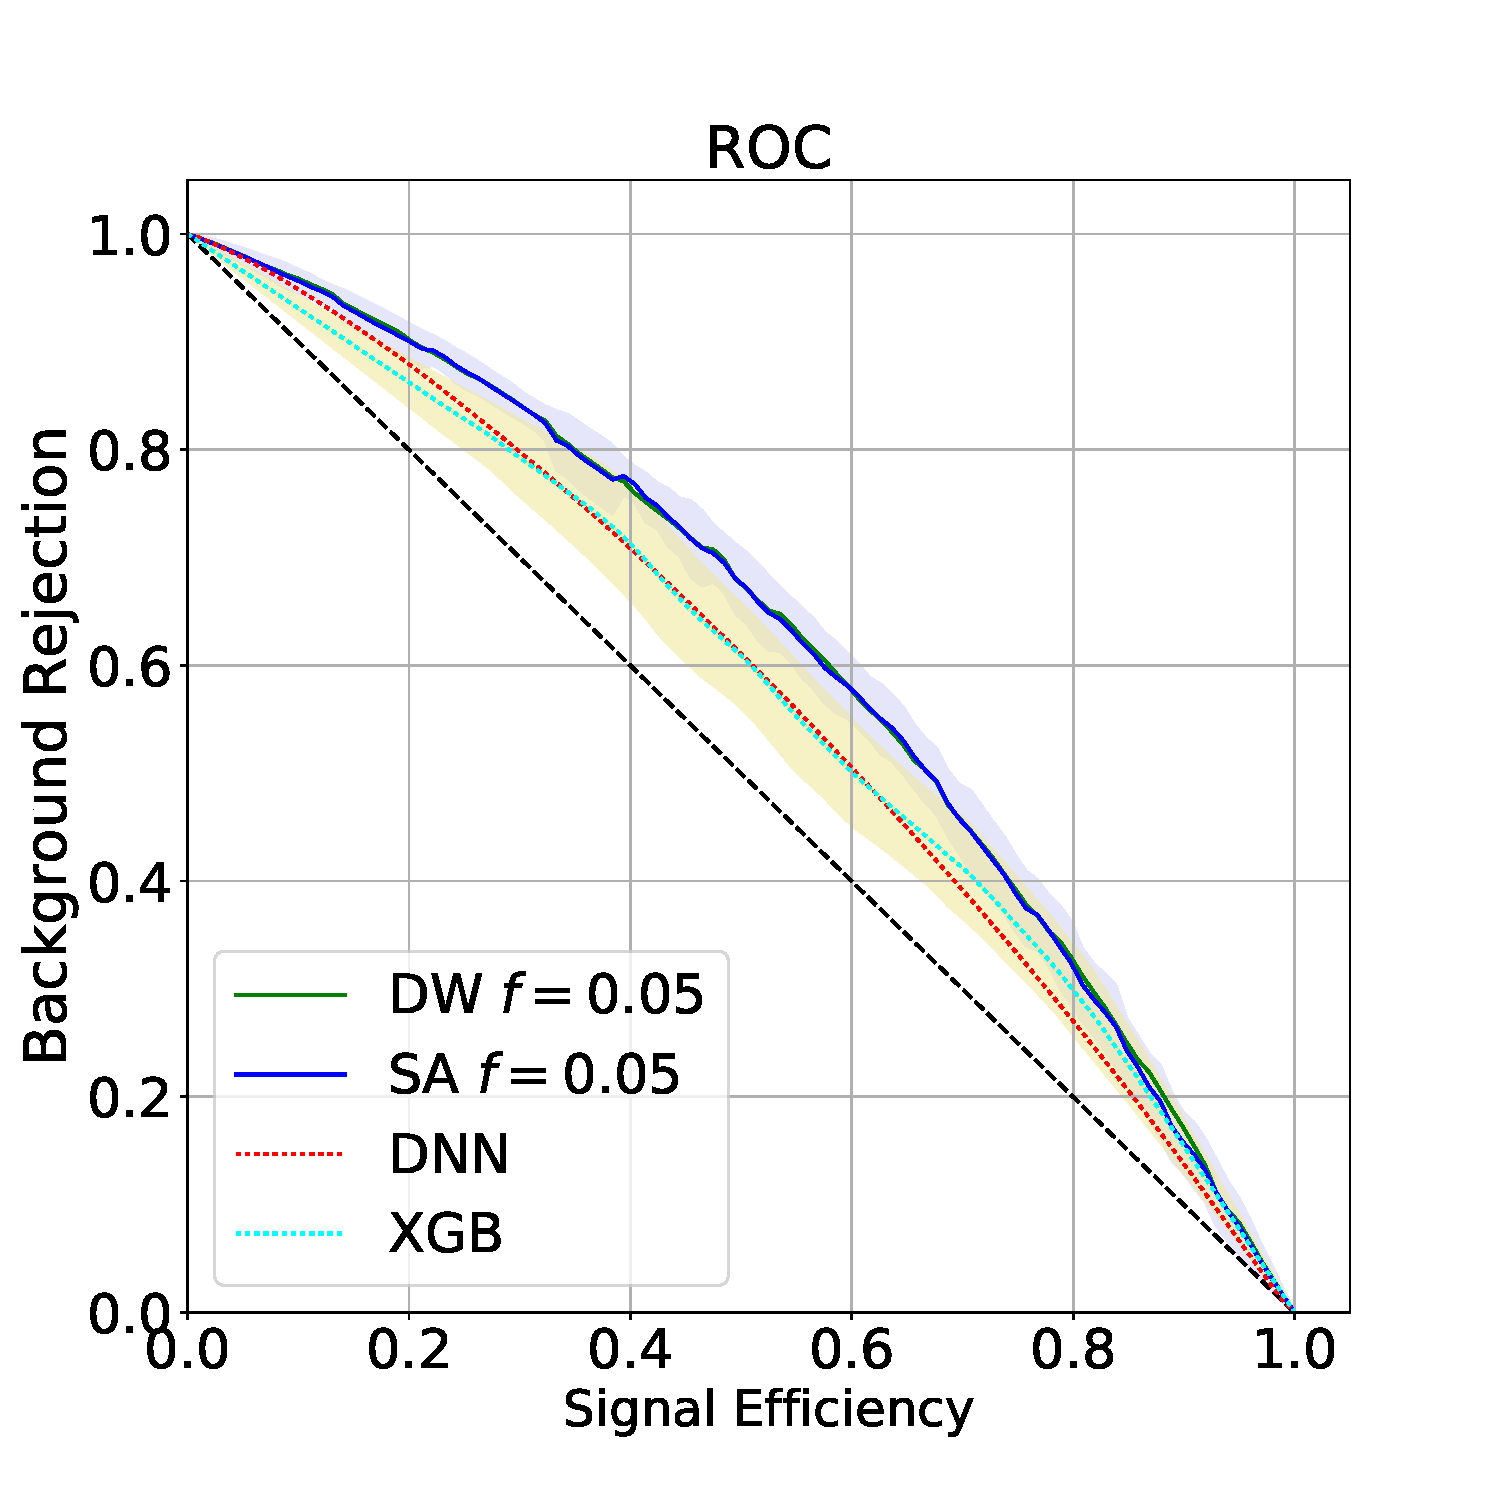
\includegraphics[width=0.49\textwidth]{ROC_example_100DWDNN}
\end{subfigure}%
\begin{subfigure}
  \centering
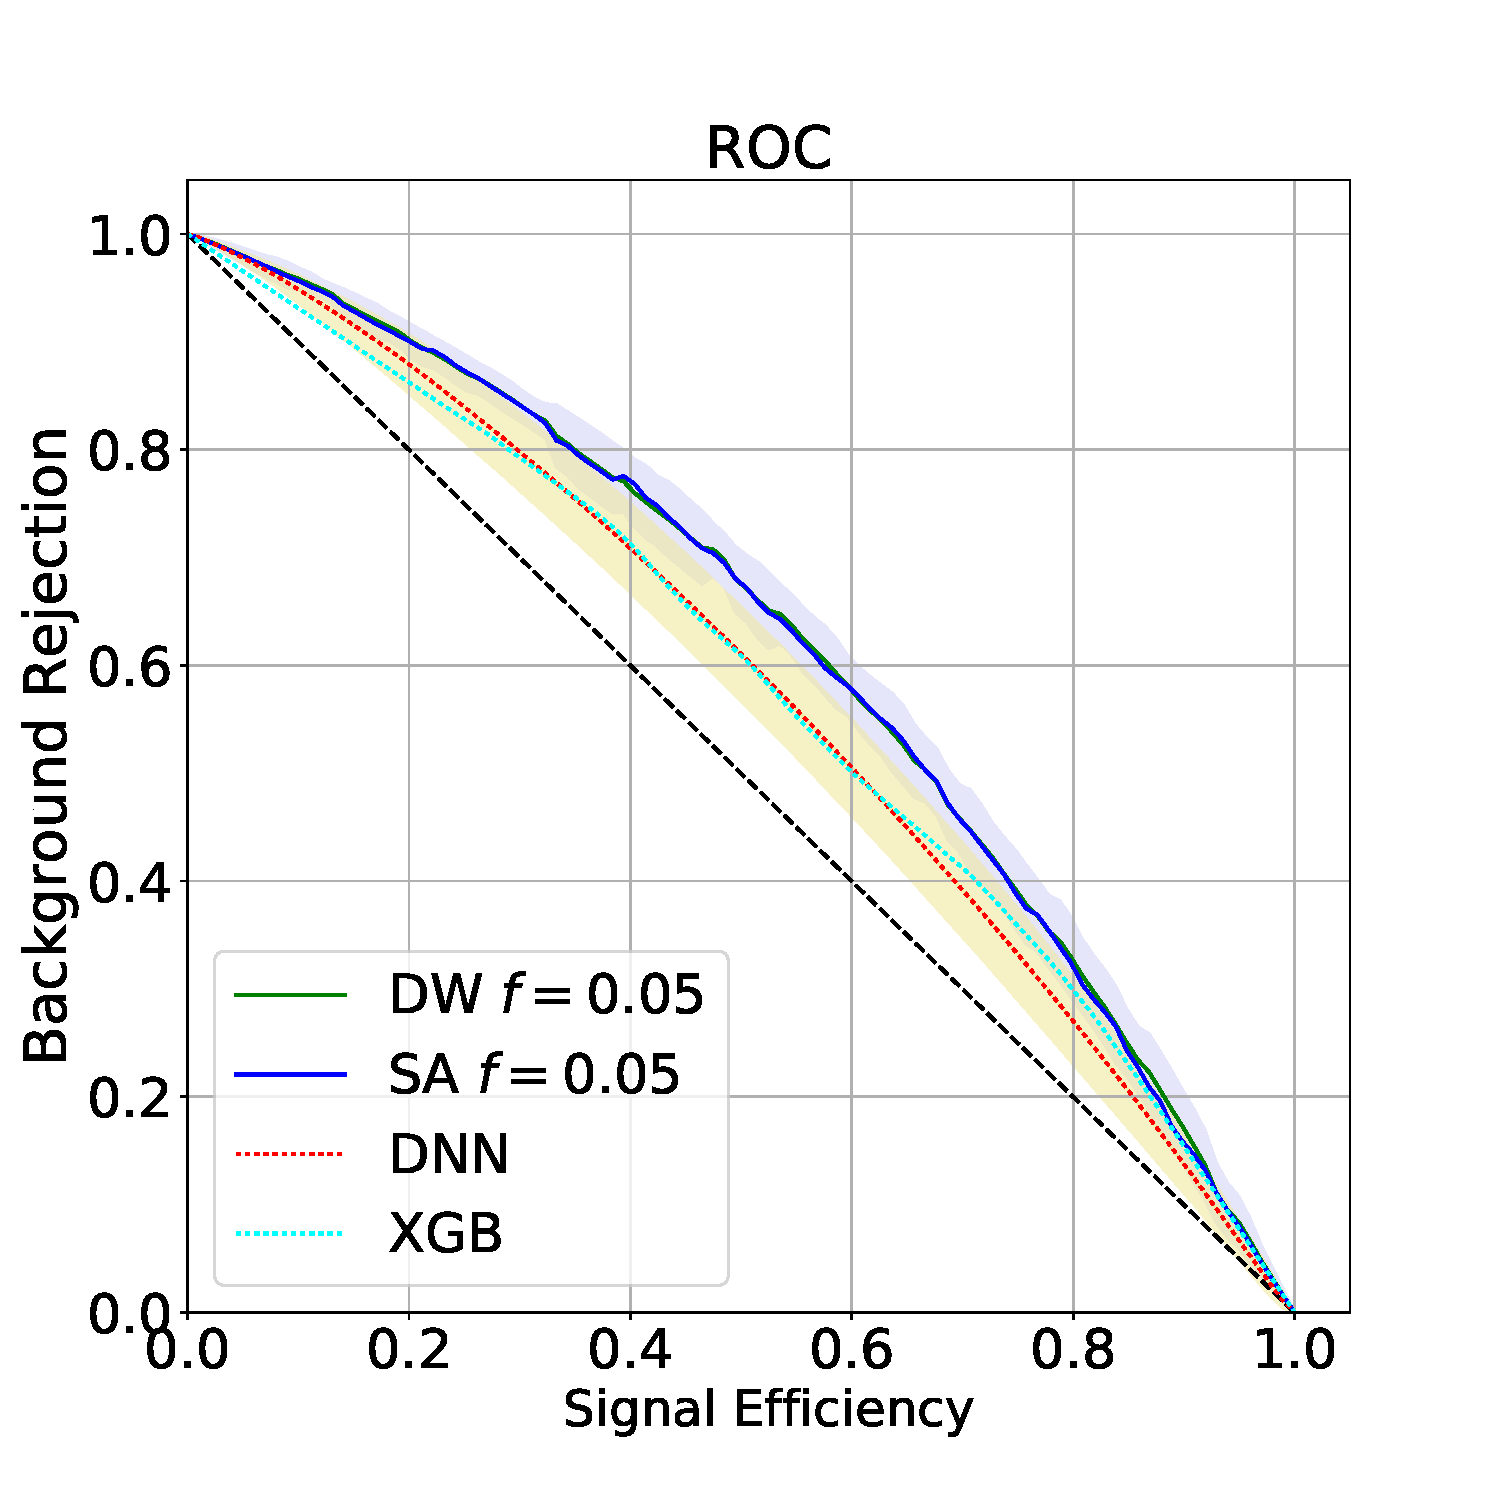
\includegraphics[width=0.49\textwidth]{ROC_example_100SAXGB}\end{subfigure}
  \caption{The ROC curves for the annealer-trained networks (DW and SA) at $f=0.05$, DNN, and XGB. Error bars are defined by the variation over the training sets and statistical error. Both panels show all four ROC curves. Panel (a) [(b)] includes $1\sigma$ error bars only for DW and DNN [SA and XGB], in light blue and pale yellow, respectively. Results shown are for the $36$ variable networks at $\lambda=0.05$ trained on $100$ events. The annealer trained networks have a larger area under the ROC curve}
 \label{fig:ROC_example}
  \end{figure}

  
\begin{figure}[hbb]
 \centering
  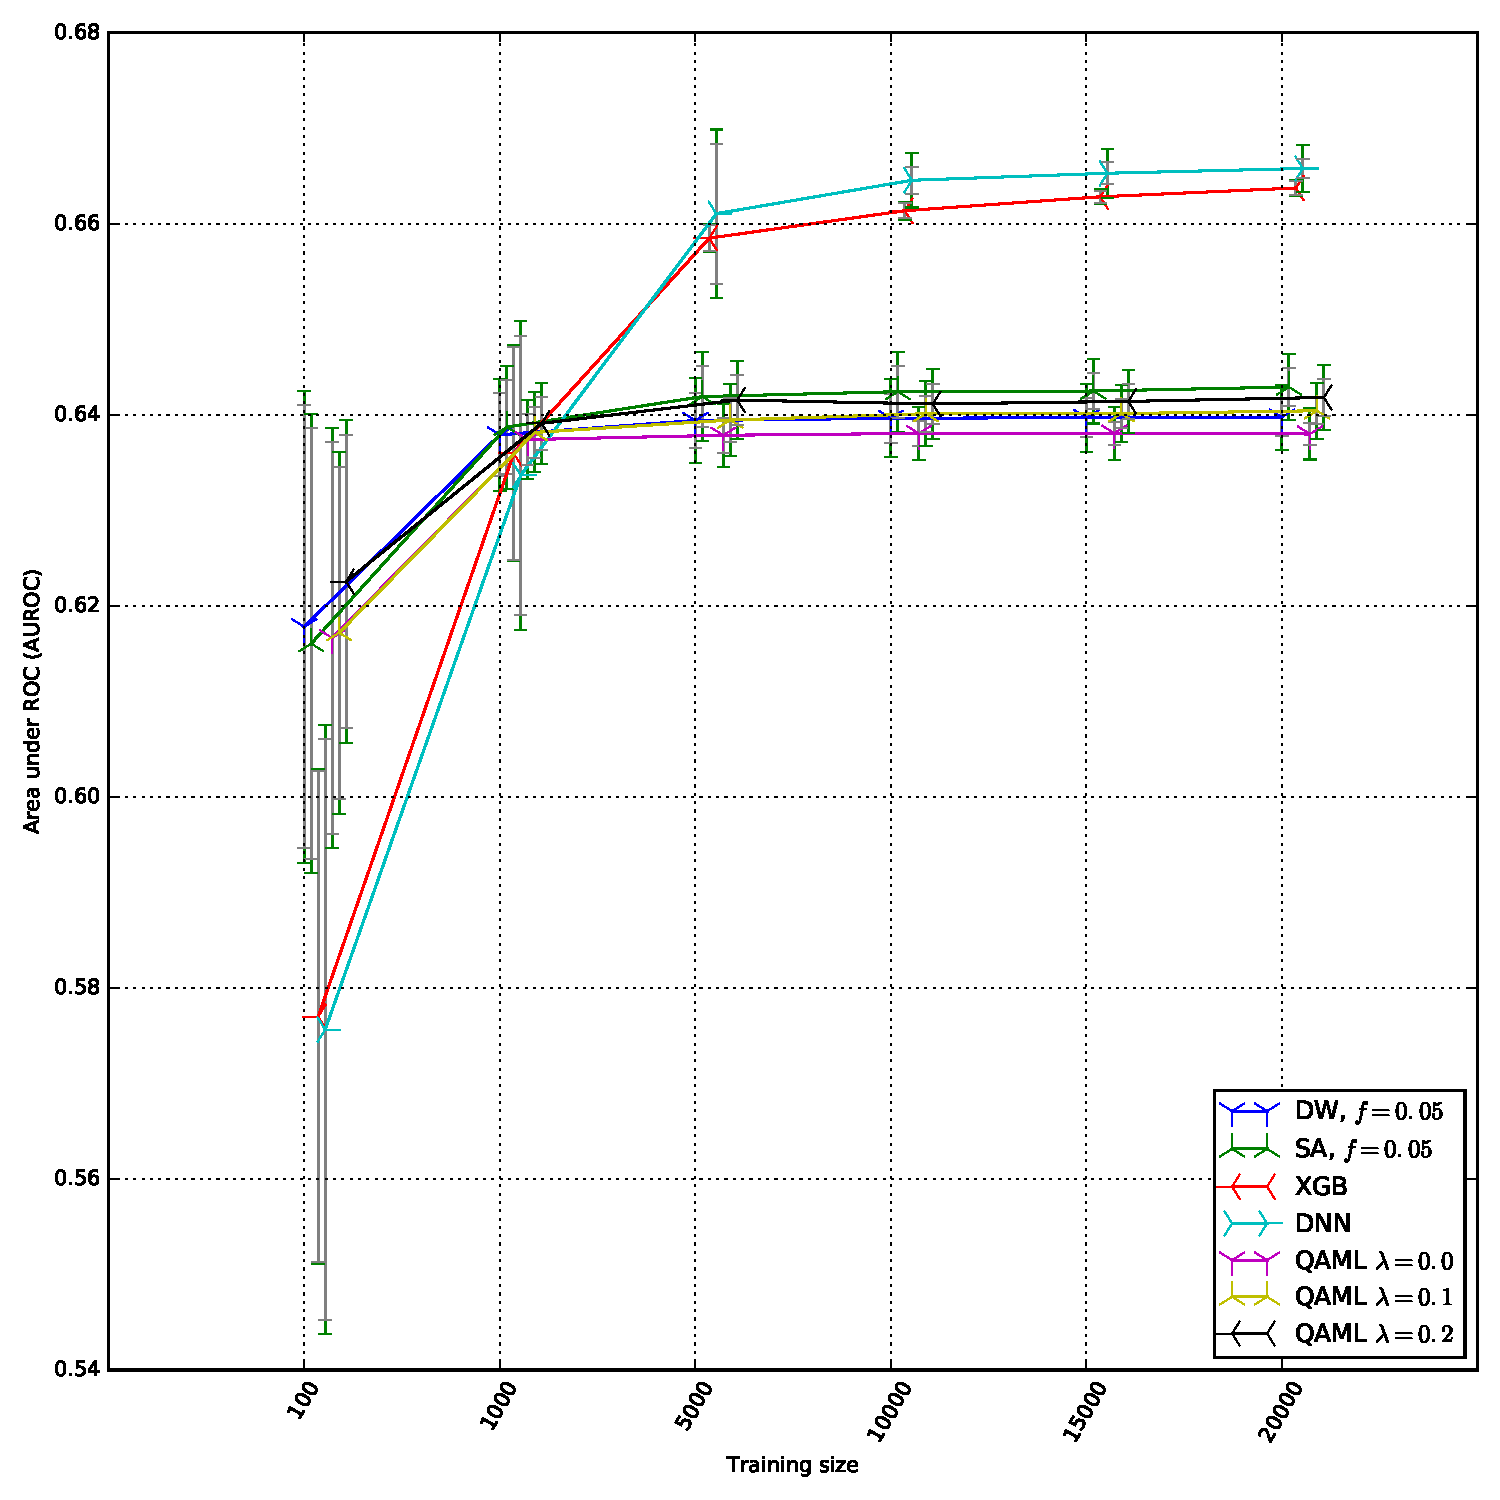
\includegraphics[width=0.7\columnwidth]{aucs_lambda}
  \caption{A reproduction of Fig.~3
  %\ref{fig:aucs} 
  from the main text, now including the optimal strong classifier found by SA at $f=0$ 
  for various values of the regularization parameter $\lambda=0.,0.1,0.2$. We find that this parameter has negligible impact on the shape of the AUROC curve, and that performance for SA always saturates at $\approx 0.64$, with an advantage for QAML (DW) and SA over XGB and DNNs for small training sizes.}
  \label{fig:aucs_lambda}
\end{figure}  

When we take $f>0$ and accept excited states with energy $E<(1-f)E_{GS}$  as ``successes'', we have a set of networks (labeled by $f$) for each training set. We simply take the supremum over the $f$-labeled set of values of $r_B$ at each value of $\epsilon_S$, to form the ROC curve for the classifier formed by pasting together different classifiers over various ranges of $\epsilon_S$. 

To estimate the error due to limited test sample statistics, we reweight each element of the test set with weights $\vec{w}$ drawn from a Poisson distribution with mean $1$, effectively computing $ \sum_i w_i p_i y_k^i$. The weights on the elements of the test set are determined for all elements at once and we  evaluate all strong classifiers using the same weights. For a single weight vector, we evaluate many values of the cut, and use linear interpolation to evaluate it in steps of 0.01 in the region $[0,1]$. This gives us the true negative rate as a function of the true positive rate for a single weighting corresponding  to a single estimated ROC curve.  When constructing a composite classifier from multiple states, we are identifying regions of signal efficiency in which one should use one of the states rather than the others, namely, we take the maximum background rejection rate over the states for each value of signal efficiency. 

Repeating for many reweightings we get many ROC curves all of which are consistent with our data, and thus the standard deviation across weights on a single training set at each value of signal efficiency serves as an estimate of the statistical uncertainty in our ROC curves.

To estimate variation due to the choice of the training set  towards  reproductions of the procedure and results, for a given training size we generate multiple disjoint training sets and use the standard deviation in mean performance across training sets as our estimate of the error on the model resulting from the particular choice of training set. When we compute the difference between two ROCs or AUROCs, we hold the training set and weight vector fixed, take the difference, and then perform statistics over the weights and training sets in the same manner as above. Errors in the AUROC were estimated similarly, taking the AUROC for each Poisson weight vector and training set (fold) instead of $r_B(\epsilon_S)$. This is the procedure leading to Fig.~3 in the main text. An example of the ROC curves is given in Fig.~\ref{fig:ROC_example}. At the scale of that plot, it is virtually impossible to tell the detailed differences between SA and DW or the various values of $f$, so we use plots of differences of AUCs to extract more detailed information about the ROC curves. This leads to Fig.~4 in the main text. Additional difference plots are given in Sec.~\ref{sec:ROC-diffs} below.
  
\section*{Quantum annealing and D-Wave}
In QA, we interpret the Ising spins $s_i$ in the Ising Hamiltonian~\eqref{eq:HIsing} as Pauli operators $\sigma_i^z$ on the ${i}^{\mathrm{th}}$ qubit in a system of $N$ qubits. QA is inspired by the adiabatic theorem,\cite{Kato:50} namely if the Hamiltonian is interpolated from an initial Hamiltonian $H(t=0)$ to a final Hamiltonian $H(t=t_a)$ sufficiently slowly compared to the minimum ground-to-first-excited state gap of $H(t)$, the system will be in the ground state of $H(t=t_a)$ with high probability, provided it was initialized in the ground state of $H(t=0)$. Thus, one can evolve from a simple, easy to initialize Hamiltonian at $t=0$ to a complicated Hamiltonian with an unknown ground state at $t=t_a$, where $t_a$ is known as the annealing time. In QA, the initial Hamiltonian is a transverse field $H_X = \sum_i \sigma_i^x$, and the final Hamiltonian is the Ising Hamiltonian~\eqref{eq:HIsing}, with the time-dependent Hamiltonian taking the form $H(t) = A(t)H_X+ B(t)H_{\mathrm{Ising}}$, where $A(t)$ is monotonically decreasing to $0$ and $B(t)$ is monotonically increasing from $0$; these functions are known as the annealing schedule. QA can be seen as both a generalization and a restriction of adiabatic quantum computation \cite{Farhi:00} (for a review see \cite{Albash-Lidar:RMP}): as a restriction, QA typically requires the initial Hamiltonian to be a sum of $\sigma^x$s and the final Hamiltonian be diagonal in the computational basis (i.e., a sum of $\sigma^z$ terms), while, as a generalization, it undergoes open-system dynamics and need not remain in the ground state for the entire computation.
  
Current and near-generation quantum annealers are naturally run in a batch mode in which one draws many samples from a single Hamiltonian. Repeated draws for QA are  fast. The DW averages approximately $5000$ samples per second under optimal conditions. We take advantage of this by keeping all the trial strong classifiers returned and not restricting to the one with minimum energy.\footnote{The energy is effectively a function of error on the training set of the weak classifiers, hence is distinct from the measures used to directly judge classifier performance, such as the area under the ROC curve.}The DW has $1098$ superconducting Josephson junction flux qubits arranged into a grid, with couplers between the qubits in the form shown in Fig.~\ref{fig:chimera}, known as the Chimera graph. The annealing schedule used in the DW processor is given in Fig.~\ref{fig:annsched}. The  Chimera graph is not fully connected, a recognized  limitation  as the Ising Hamiltonian~\eqref{eq:HIsing} is fully connected, in general. To address this, we perform a {\it minor embedding operation}~\cite{Choi1,Choi2}. Minor embedding is the process whereby we map a single logical qubit in $H_{\mathrm{Ising}}$ into a physical ferromagnetic ($J_{ij}=-1$) chain of qubits on DW. 
For each instance we use a heuristic embedding found via the D-Wave API, that is as regular and space-efficient as possible for our problem sizes. 
 
 \begin{figure}[hbt]
 \centering
  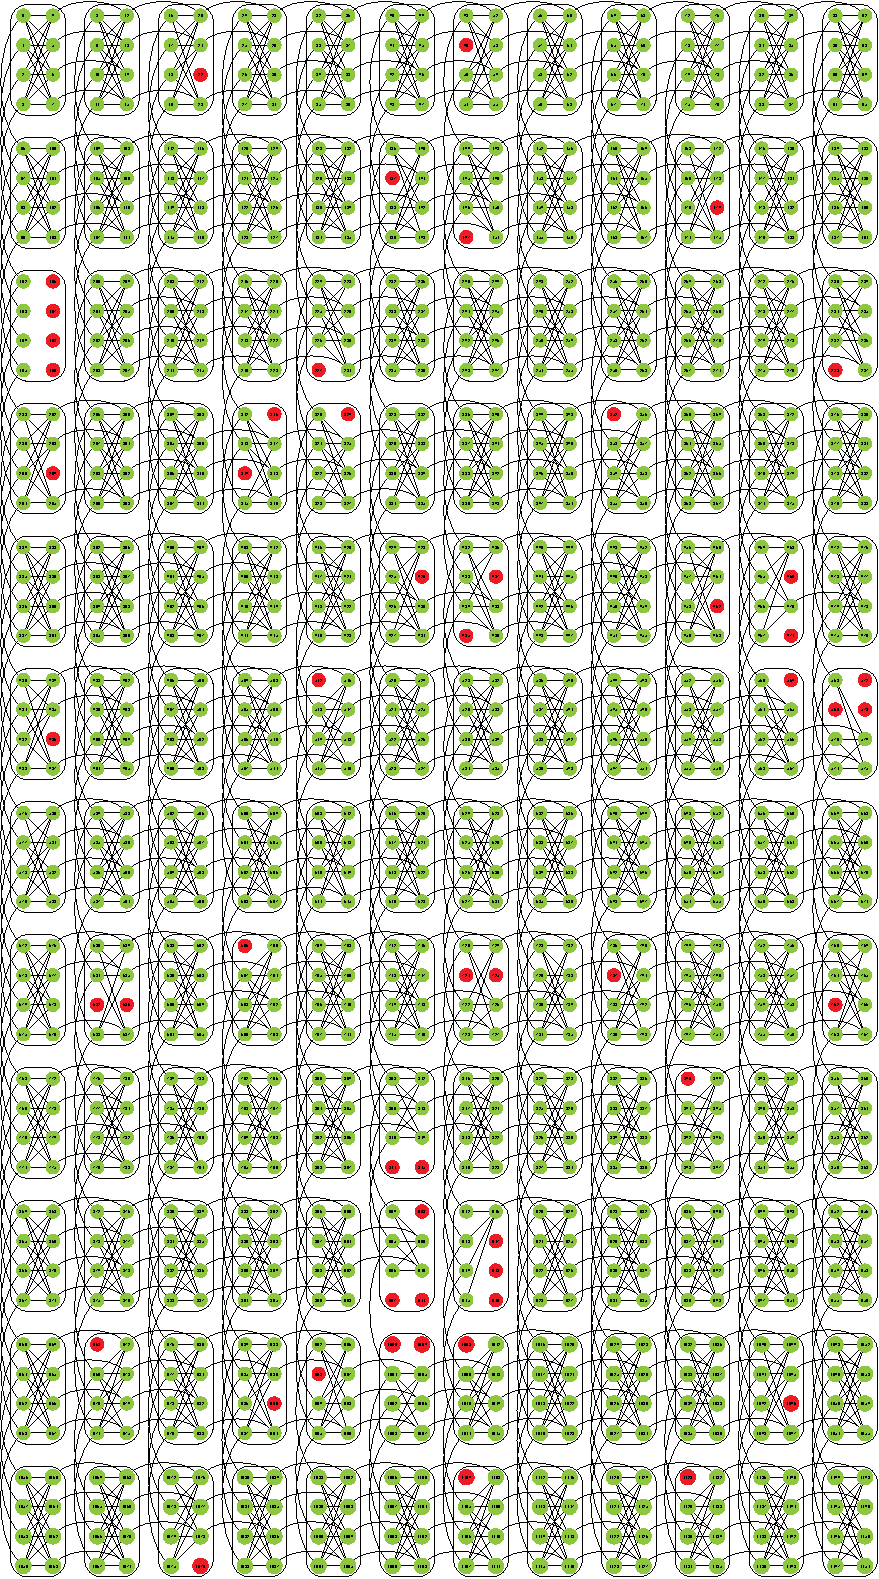
\includegraphics[width=.7\columnwidth]{chimera.pdf}
  \caption{An $1152$ qubit Chimera graph, partitioned into a $12\times 12$ array of $8$-qubit unit cells, each unit cell being a $K_{4,4}$ bipartite graph. Inactive qubits are marked in red, active qubits in green. There are a total of $1098$ active qubits in the DW processor used in our experiments. Black lines denote active couplers.}
  \label{fig:chimera}
\end{figure}

 \begin{figure}[hbt]
 \centering
  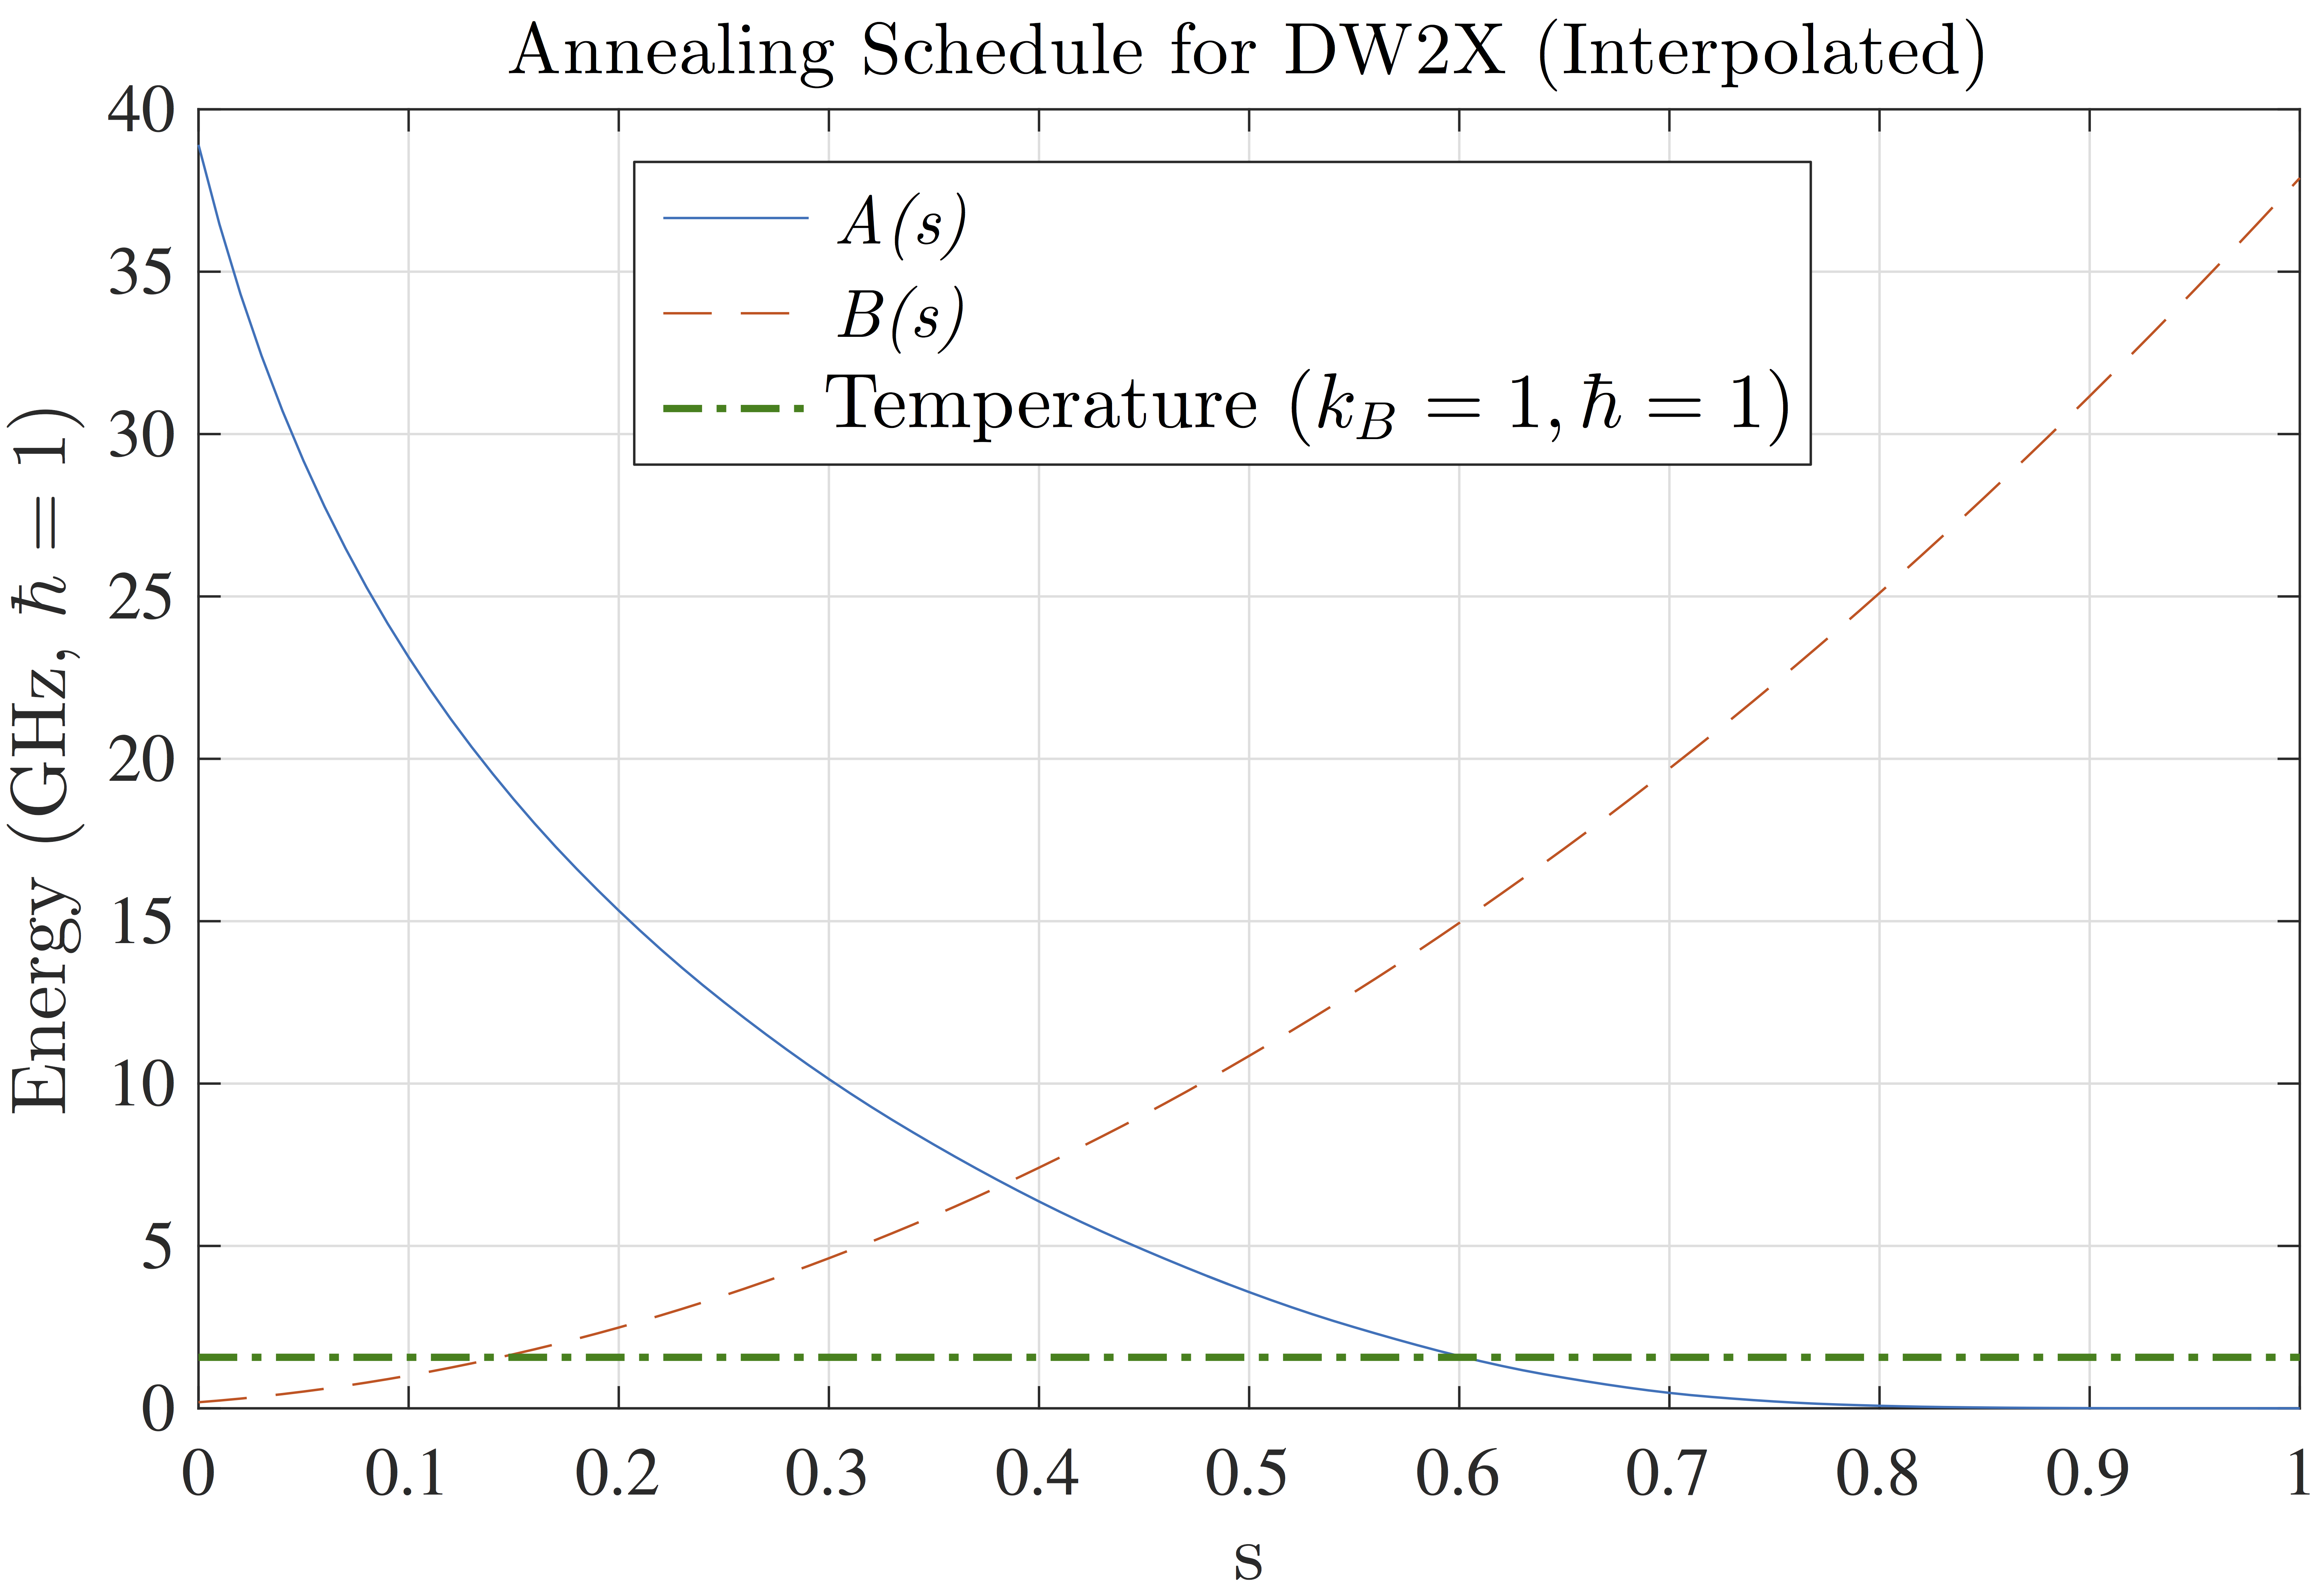
\includegraphics[width=0.7\columnwidth]{AnnealingSchedule}
  \caption{Annealing schedule used in our experiments.}
  \label{fig:annsched}
  \end{figure}
 
Given a minor embedding map of logical qubits into a chain of physical qubits, we divide the local fields $h_i$ equally among all the qubits making up the chain for logical qubit $i$, and divide $J_{ij}$ equally among all the physical couplings between the chains making up logical qubits $i$ and $j$. After this procedure, there remains a final degree of freedom: the chain strength $J_F$. If the strength of the couplers in the ferromagnetic chains making up logical qubits is defined to be $1$, then the maximum magnitude of any other coupler is $\max\big(\max_i(\{\abs{h_i}\}),\max_{i,j}(\{\abs{J_{ij}}\})\big) = \frac{1}{J_F}$. There is an optimal value of $J_F$, generally. This is due to a competition between the chain needing to behave as a single large qubit and the problem Hamiltonian needing to drive the dynamics\cite{Venturelli:2014nx}. If $J_F$ is very large, the chains will ``freeze out'' long before the logical problem, i.e., the chains will be far stronger than the problem early on, and the transverse field terms will be unable to induce the large, multi-qubit flipping events necessary to explore the logical problem space. Similarly, if $J_F$ is very weak, the chains will be broken (i.e., develop a kink or domain wall) by tension induced by the problem, or by thermal excitations, and so the system will generally not find very good solutions. Ideally, one wants the chains and the logical problem to freeze at the same time, so that at the critical moment in the evolution both constraints act simultaneously to determine the dynamics. For the results shown here, we used $J_F=6$ with an annealing time $t_a=5\mu$s. To deal with broken chains, we use majority vote on the chain with a coin-toss tie-breaker for even length chains.  Detailed analysis of the performance of this strategy in the context of error correction can be found in the literature~\cite{Vinci:2015jt,Mishra:2015}.

Figure~\ref{fig:average_energy_by_J} shows the average minimum energy returned by the DW, rescaled by the training size (to remove a linear scaling), as a function of the chain strength and training size. We see that the smallest training size ($N=100$) has a smaller average minimum energy than the rest of the training sizes, and that there is only a very slight downward tendency as the chain strength $J_F$ increases for the larger training sizes. 

Figure~\ref{fig:minimum_fractional_residual_energy} plots the fractional deviation of the minimum energy returned by the DW relative to the true ground state energy, averaged over the training sets. While the DW's minimum energy returned approaches the true ground state, it seems to converge to $\approx 5\%$ (i.e. $f\approx0.05$) above the ground state as we increase the chain strength,  for all training sizes $\geq 1000$. In this case, we were not able to find the optimal chain strength in a reasonable range of chain strengths, and instead simply took the best we found, $J_F=6$. As discussed in Sec.~\ref{app:ICE}, the DW processor suffers from noise sources on the couplers and thermal fluctuations, and it seems that this poses significant challenges for the performance of the quantum annealer. It is possible that even larger chain strengths may resolve the issue, but given the convergence visible in Fig.~\ref{fig:minimum_fractional_residual_energy}, it seems likely that $J_F=6$ is already near the optimum.


  \begin{figure}[hbb]
 \centering
  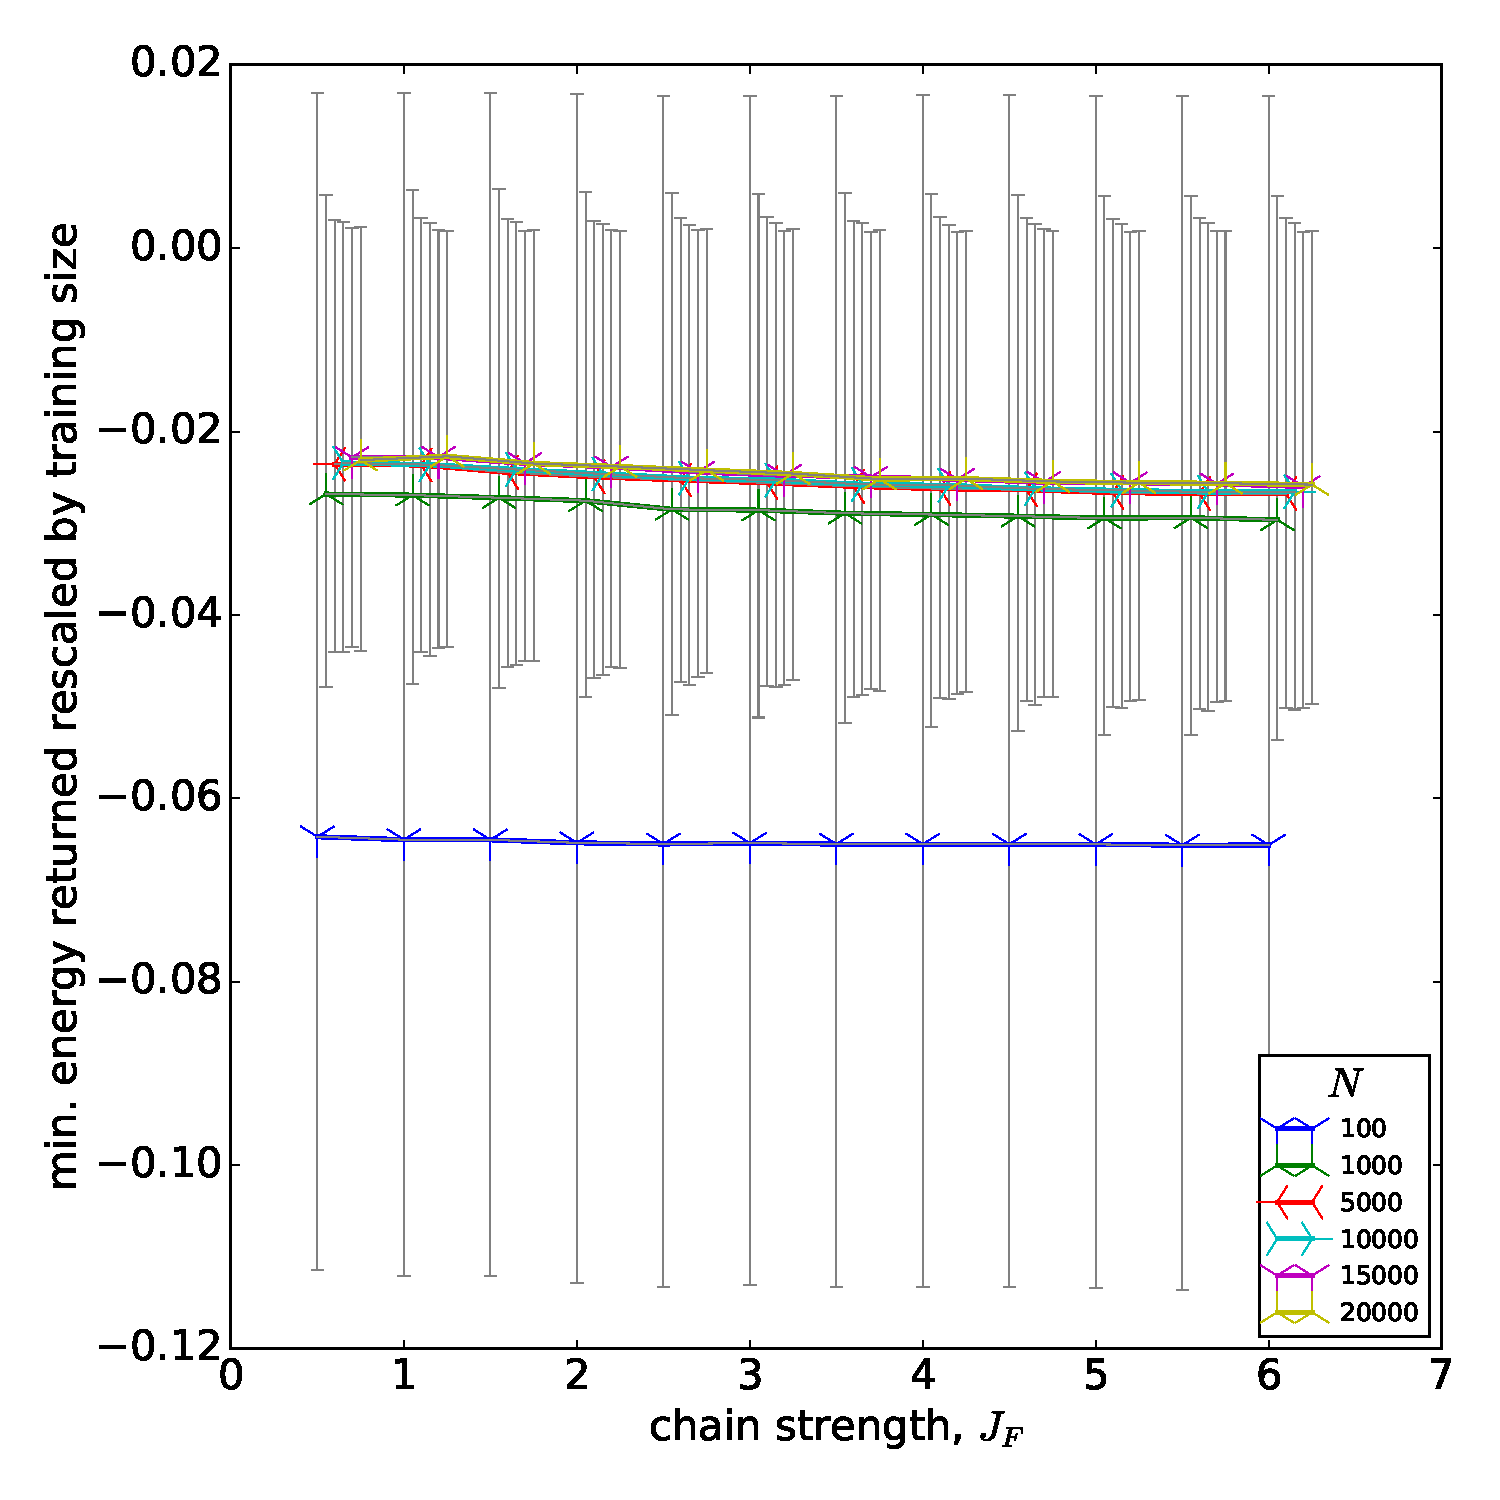
\includegraphics[width=0.7\columnwidth]{rescaled_average_return_energy_by_J}
  \caption{A plot of the minimum energy returned by the DW as a function of chain strength, rescaled by the number of training samples. I.e., for training size $N$, we plot $E_m/N$ for minimum return energy $E_m$, where $N$ is given in the legend.}
  \label{fig:average_energy_by_J}
\end{figure}
 
 \begin{figure}[hbb]
 \centering
  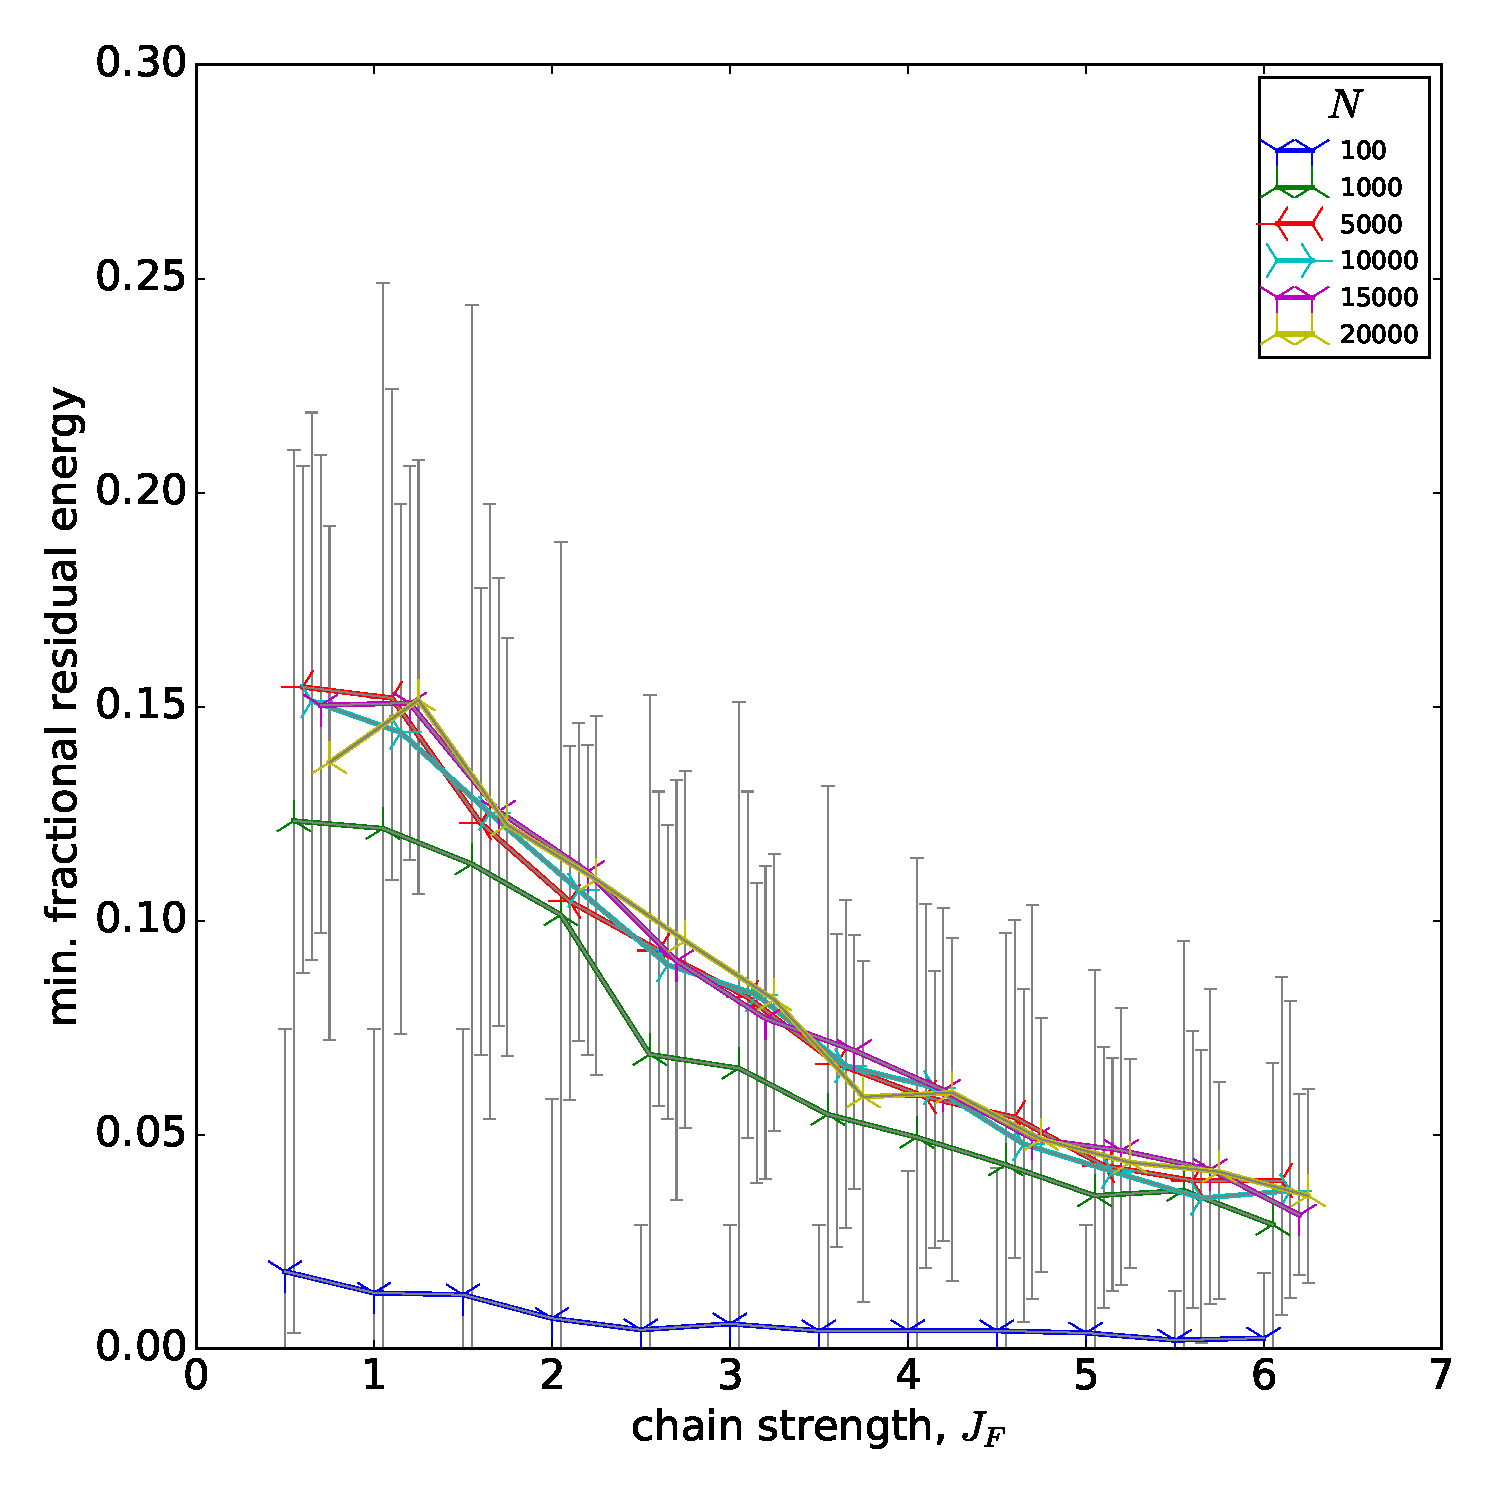
\includegraphics[width=0.7\columnwidth]{minimum_fractional_residual_energy_by_J}
  \caption{Plot of $(E_m-E_0)/E_0$ for minimum energy returned $E_m$ and true ground state energy $E_0$, i.e., the minimum fractional reserve energy, averaged over the training sets, for each size and chain strength.}
  \label{fig:minimum_fractional_residual_energy}
\end{figure}

 
\section*{Simulated annealing}
In simulated annealing,\cite{kirkpatrick_optimization_1983} we initialize the vector $\vec{s}$ in a random state. At each time step, we create a trial vector $\vec{s}'$ by flipping one of the spins in $\vec{s}$, selected at random. We accept the trial vector using the Metropolis update rule:\cite{Metropolis} the new state is accepted with probability $1$ if $H(\vec{s}')<H(\vec{s})$ (i.e., lower energy states are accepted deterministically), whereas if $H(\vec{s}')>H(\vec{s})$, we accept the trial vector with probability $\exp{-\beta(H(\vec{s}')-H(\vec{s}))}$ for some inverse temperature $\beta$. After we have attempted $N$ spin flips,
which amounts to one sweep, we then increase the inverse temperature $\beta$ according to some schedule. At first, $\beta \ll 1$ and the system quickly drifts through the space of possible states. As $\beta$ grows the system settles into lower lying valleys in the energy landscape, and ultimately ceases to evolve entirely in the limit of infinite $\beta$ (zero temperature). Our simulations used $\beta_{\mathrm{init}}=0.1$ and $\beta_{\mathrm{final}} = 5$, and used a linear annealing schedule (i.e., if we perform $S$ sweeps, we increase $\beta$ after each sweep by $\frac{\beta_{\mathrm{final}}-\beta_{\mathrm{init}}}{S}$). These parameters have generally performed well in other studies.\cite{Hen:2015rt} All SA data in the main text and presented here is at 1000 sweeps, however we also tested SA at 100 sweeps, and found a negligible difference in overall performance, as seen in Fig.~\ref{fig:SAmSA100droc}, where the integrated difference of the ROC curves is found to be statistically indistinguishable from $0$.

 \begin{figure}[hbb]
 \centering
  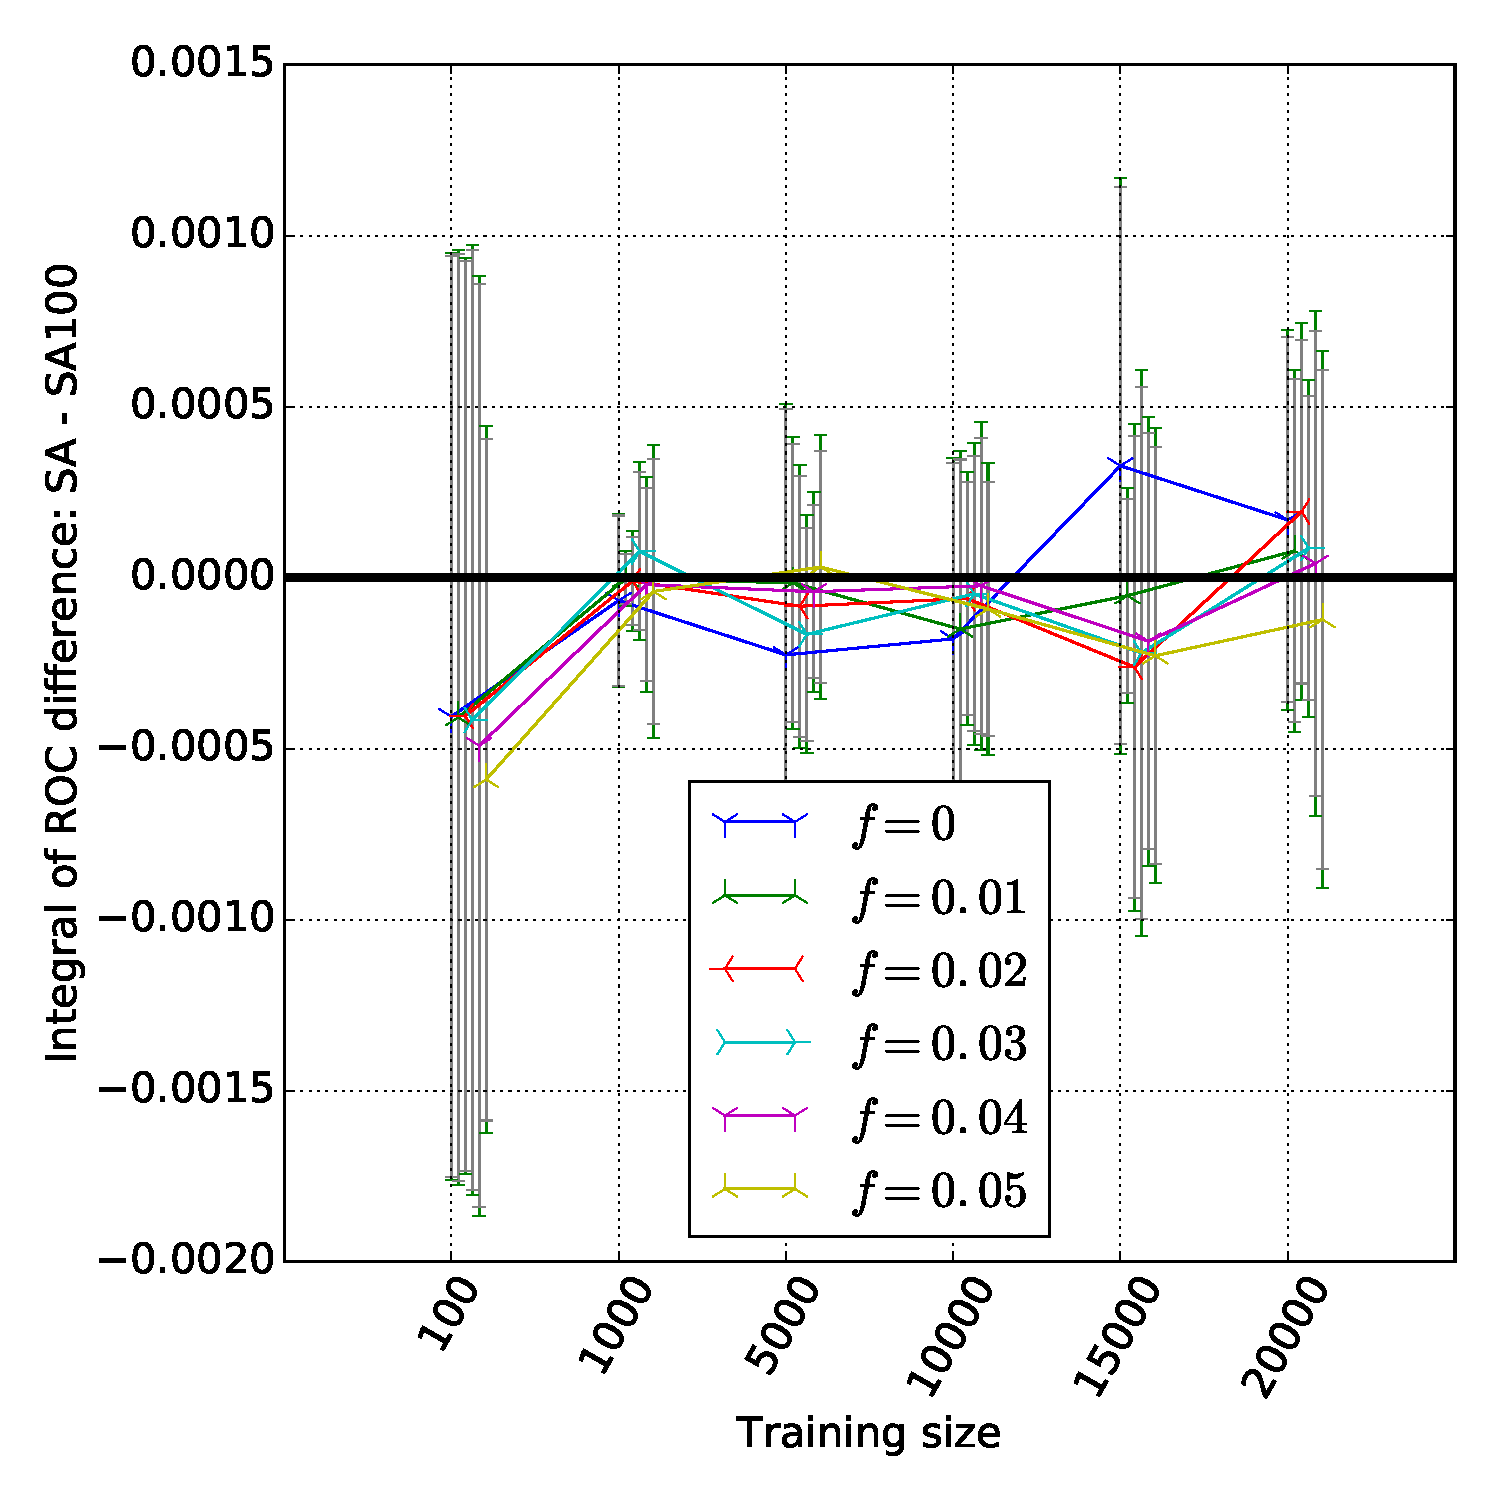
\includegraphics[width=0.7\columnwidth]{SA--SA100_auc}
  \caption{The integral of the difference of the ROC curves, i.e., the area between the ROC curves, for SA and SA100 for various thresholds of the energy and training size. SA at $100$ and $1000$ sweeps are effectively identical by this benchmark.}
  \label{fig:SAmSA100droc}
\end{figure}

 
\section*{Effect of noise on processor}
\label{app:ICE}
Internal control error (ICE) on the current generation of D-Wave processors is effectively modeled as a Gaussian centered on the problem-specified value of each coupler and local field, with standard deviation $0.025$, i.e., a coupler $J_{ij}$ is realized as a value drawn from the distribution $N(J_{ij},0.025)$ when one programs a Hamiltonian. Figure~\ref{fig:noisyJ} contains a histogram of the ideal values of the embedded couplers corresponding to connections between logical qubits across all $20$ problem instances of $36$ variables at 20000 training events. One can see that the ideal distribution has some structure, with two peaks. However, if one resamples values from the Gaussian distribution induced by ICE, one finds that many of the features are washed out completely. This suggests that the explanation for the flattening out of the performance of QA as a function of training size (recall Fig.~3 in the main text) is due to this noise issue. Thus we investigate this next.

Figures~\ref{fig:precision_un}-\ref{fig:precision2} tell the story of the scaling of the couplers with training size. Figure~\ref{fig:precision_un} shows linear scaling of the maximum Hamiltonian coefficient with training size. 
We observe wider variation at the smallest training sizes, but overall the precision scales linearly with training size. This is confirmed in Figure \ref{fig:precision}, which shows the maximum coefficient normalized by the training size. Since this value is constant for sufficiently large training sizes, the maximum value scales linearly with size. 
%
At first glance, this indeed suggests an explanation for why the performance of QA using the DW levels off as a function of training size: the coupling values pass $20$ (half the scale of the errors which is $\approx 1/0.025=40$). However, absolute numbers are not necessarily informative, and  Fig.~\ref{fig:precision2} dispels this explanation.

Figure~\ref{fig:precision2} shows the ratio of the median coefficient to the maximum coefficient, thereby showing the scale of \emph{typical} Hamiltonian coefficients on the DW prior to rescaling for chain strength (which for the most of the data here would reduce the magnitude by a further factor of $6$). 
 
Since all the different types of coefficient ratios are constant with system size, we have effectively no scaling with training size of the precision of the couplers. This means that the scaling of precision with training size cannot explain the saturation of performance with increasing training size.


However, the magnitudes here are quite small, and so once one accounts for rescaling the energies, typical couplers are expected to be subject to a significant amount of noise, even causing them to change sign. This effect likely explains, at least in part, the difficulties the DW has in finding the true ground state, as discussed above and seen in Fig.~\ref{fig:minimum_fractional_residual_energy}, where even at the largest chain strength we still find that the DW's typical minimum energy is $\sim 5\%$ above the ground state energy.


\begin{figure}
\centering
\begin{subfigure}
  \centering
  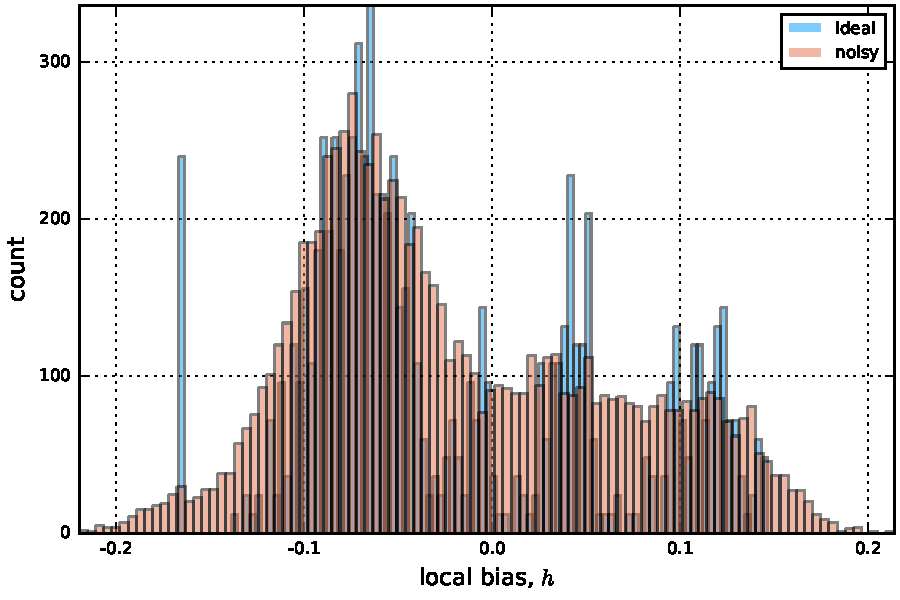
\includegraphics[width=.8\linewidth]{noisy_couplers_h}
\end{subfigure}%
\begin{subfigure}
  \centering
  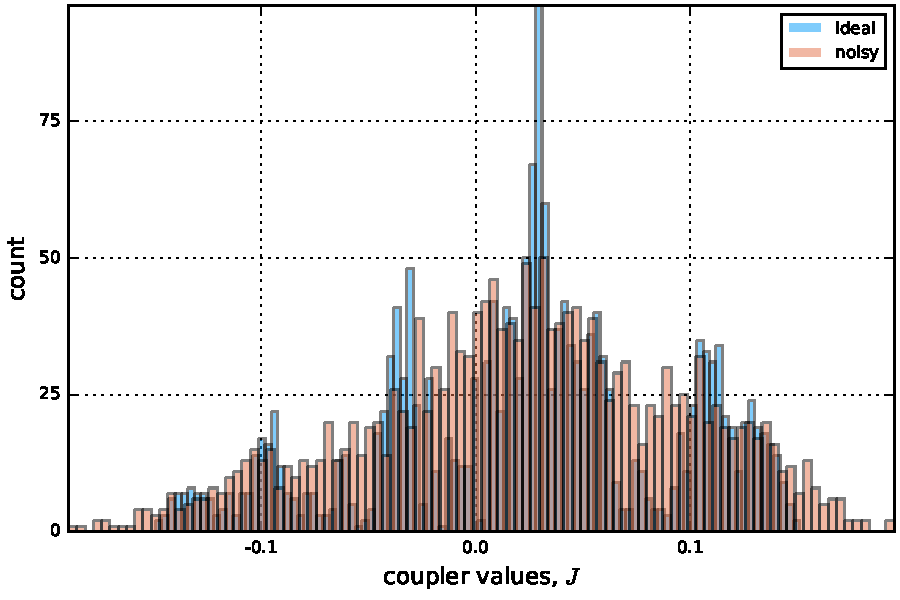
\includegraphics[width=.8\linewidth]{noisy_couplers_J}
\end{subfigure}
\caption{Histograms for the true (peaked) distribution of local biases and couplers, and the same distribution subject to point-wise Gaussian noise with zero mean and standard deviation $0.025$, which is approximately the magnitude of errors on the DW couplers.}
  \label{fig:noisyJ}
  \end{figure}

  \begin{figure}[hbb]
 \centering
  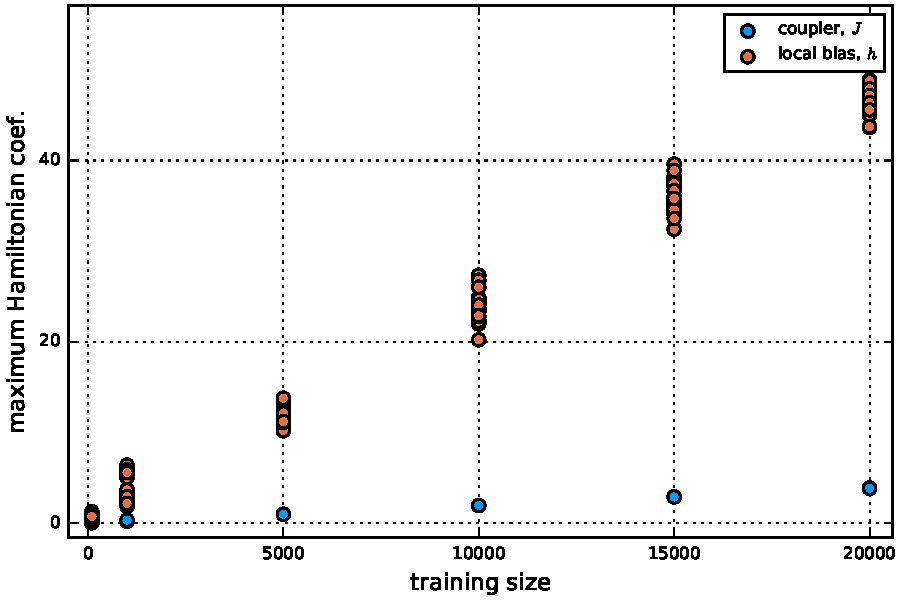
\includegraphics[width=0.7\columnwidth]{precision_by_training_size_and_fold_unnormalized}
  \caption{The maximum local bias and coupler term in the Hamiltonian across training sizes and training sets.}
  \label{fig:precision_un}
\end{figure}
 
 \begin{figure}[hbb]
 \centering
  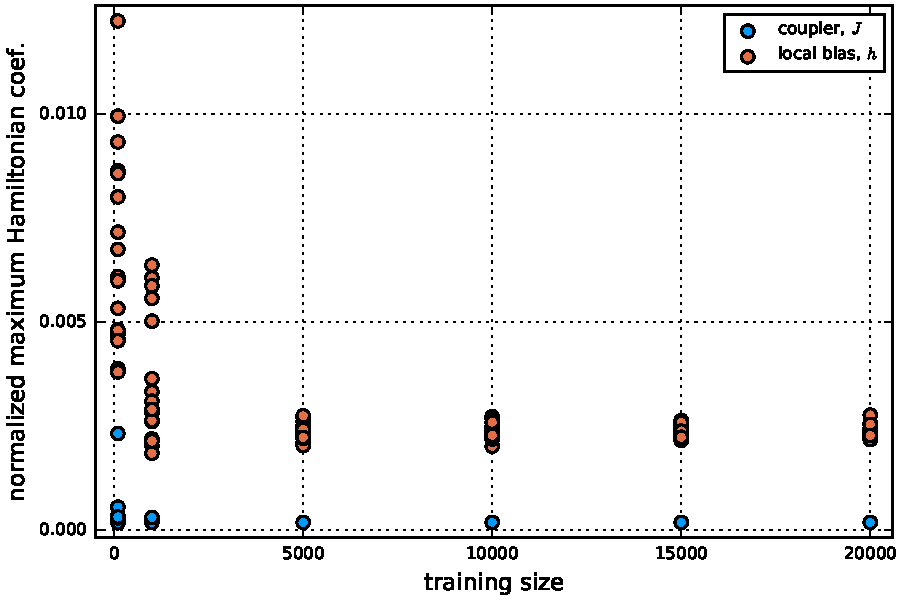
\includegraphics[width=0.7\columnwidth]{precision_by_training_size_and_fold}
  \caption{The maximum local bias and coupler term in the Hamiltonian across training sizes and training sets, normalized by the number of events in the training set. This makes it clear that the scaling of the Hamiltonian coefficients is linear in the training size, for training sizes $\geq 5000$.}
  \label{fig:precision}
\end{figure}

 \begin{figure}[hbb]
 \centering
  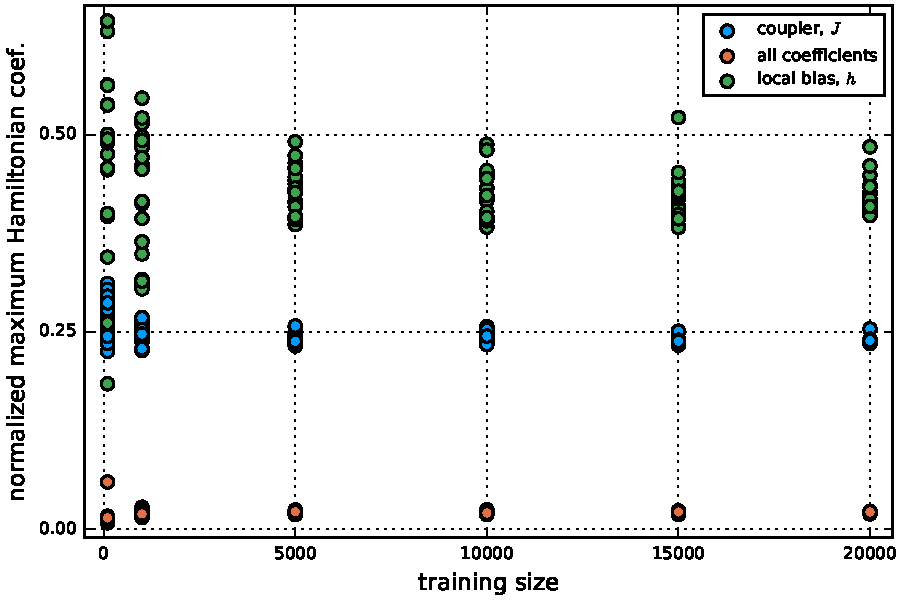
\includegraphics[width=0.7\columnwidth]{precision_by_training_size_and_fold_med_to_max}
  \caption{The ratio of the median coefficient by the maximum coefficient for the non-zero local biases, couplers, and both taken together. 
}
  \label{fig:precision2}
\end{figure}


\section*{Sensitivity to variation of the parameters of weak classifier construction}
When constructing the weak classifiers, we choose to define $v_{\text{cut}}$ as the $70$th percentile of the signal distribution. This choice is arbitrary. To test the  effect of this value  on the classifier performance we use  identical training sets and values of both $60\%$ and $80\%$ and compare  them to our primary estimate of $70\%$. The results for both the minimum energy returned ($f=0$) and $f=0.05$ for each are shown in Fig.~\ref{fig:droc_vcut6070}.

Note that every training set has the same ground state configuration at $70\%$ and $80\%$. The ROCs and AUROC are  then invariant  across a wide range of $v_{\text{cut}}$ values. 

Figure~\ref{fig:aucs_lambda} reproduces Fig.~3 
from the main text, but
also shows the AUROC for SA's optimal classifier (by energy) for various values of the regularization parameter $\lambda$. We find no significant variation, with the major features of SA being stable, namely the advantage at small training size and the saturation at around an AUROC of $\approx 0.64$.

\begin{figure}[h]
\centering
\begin{subfigure}\centering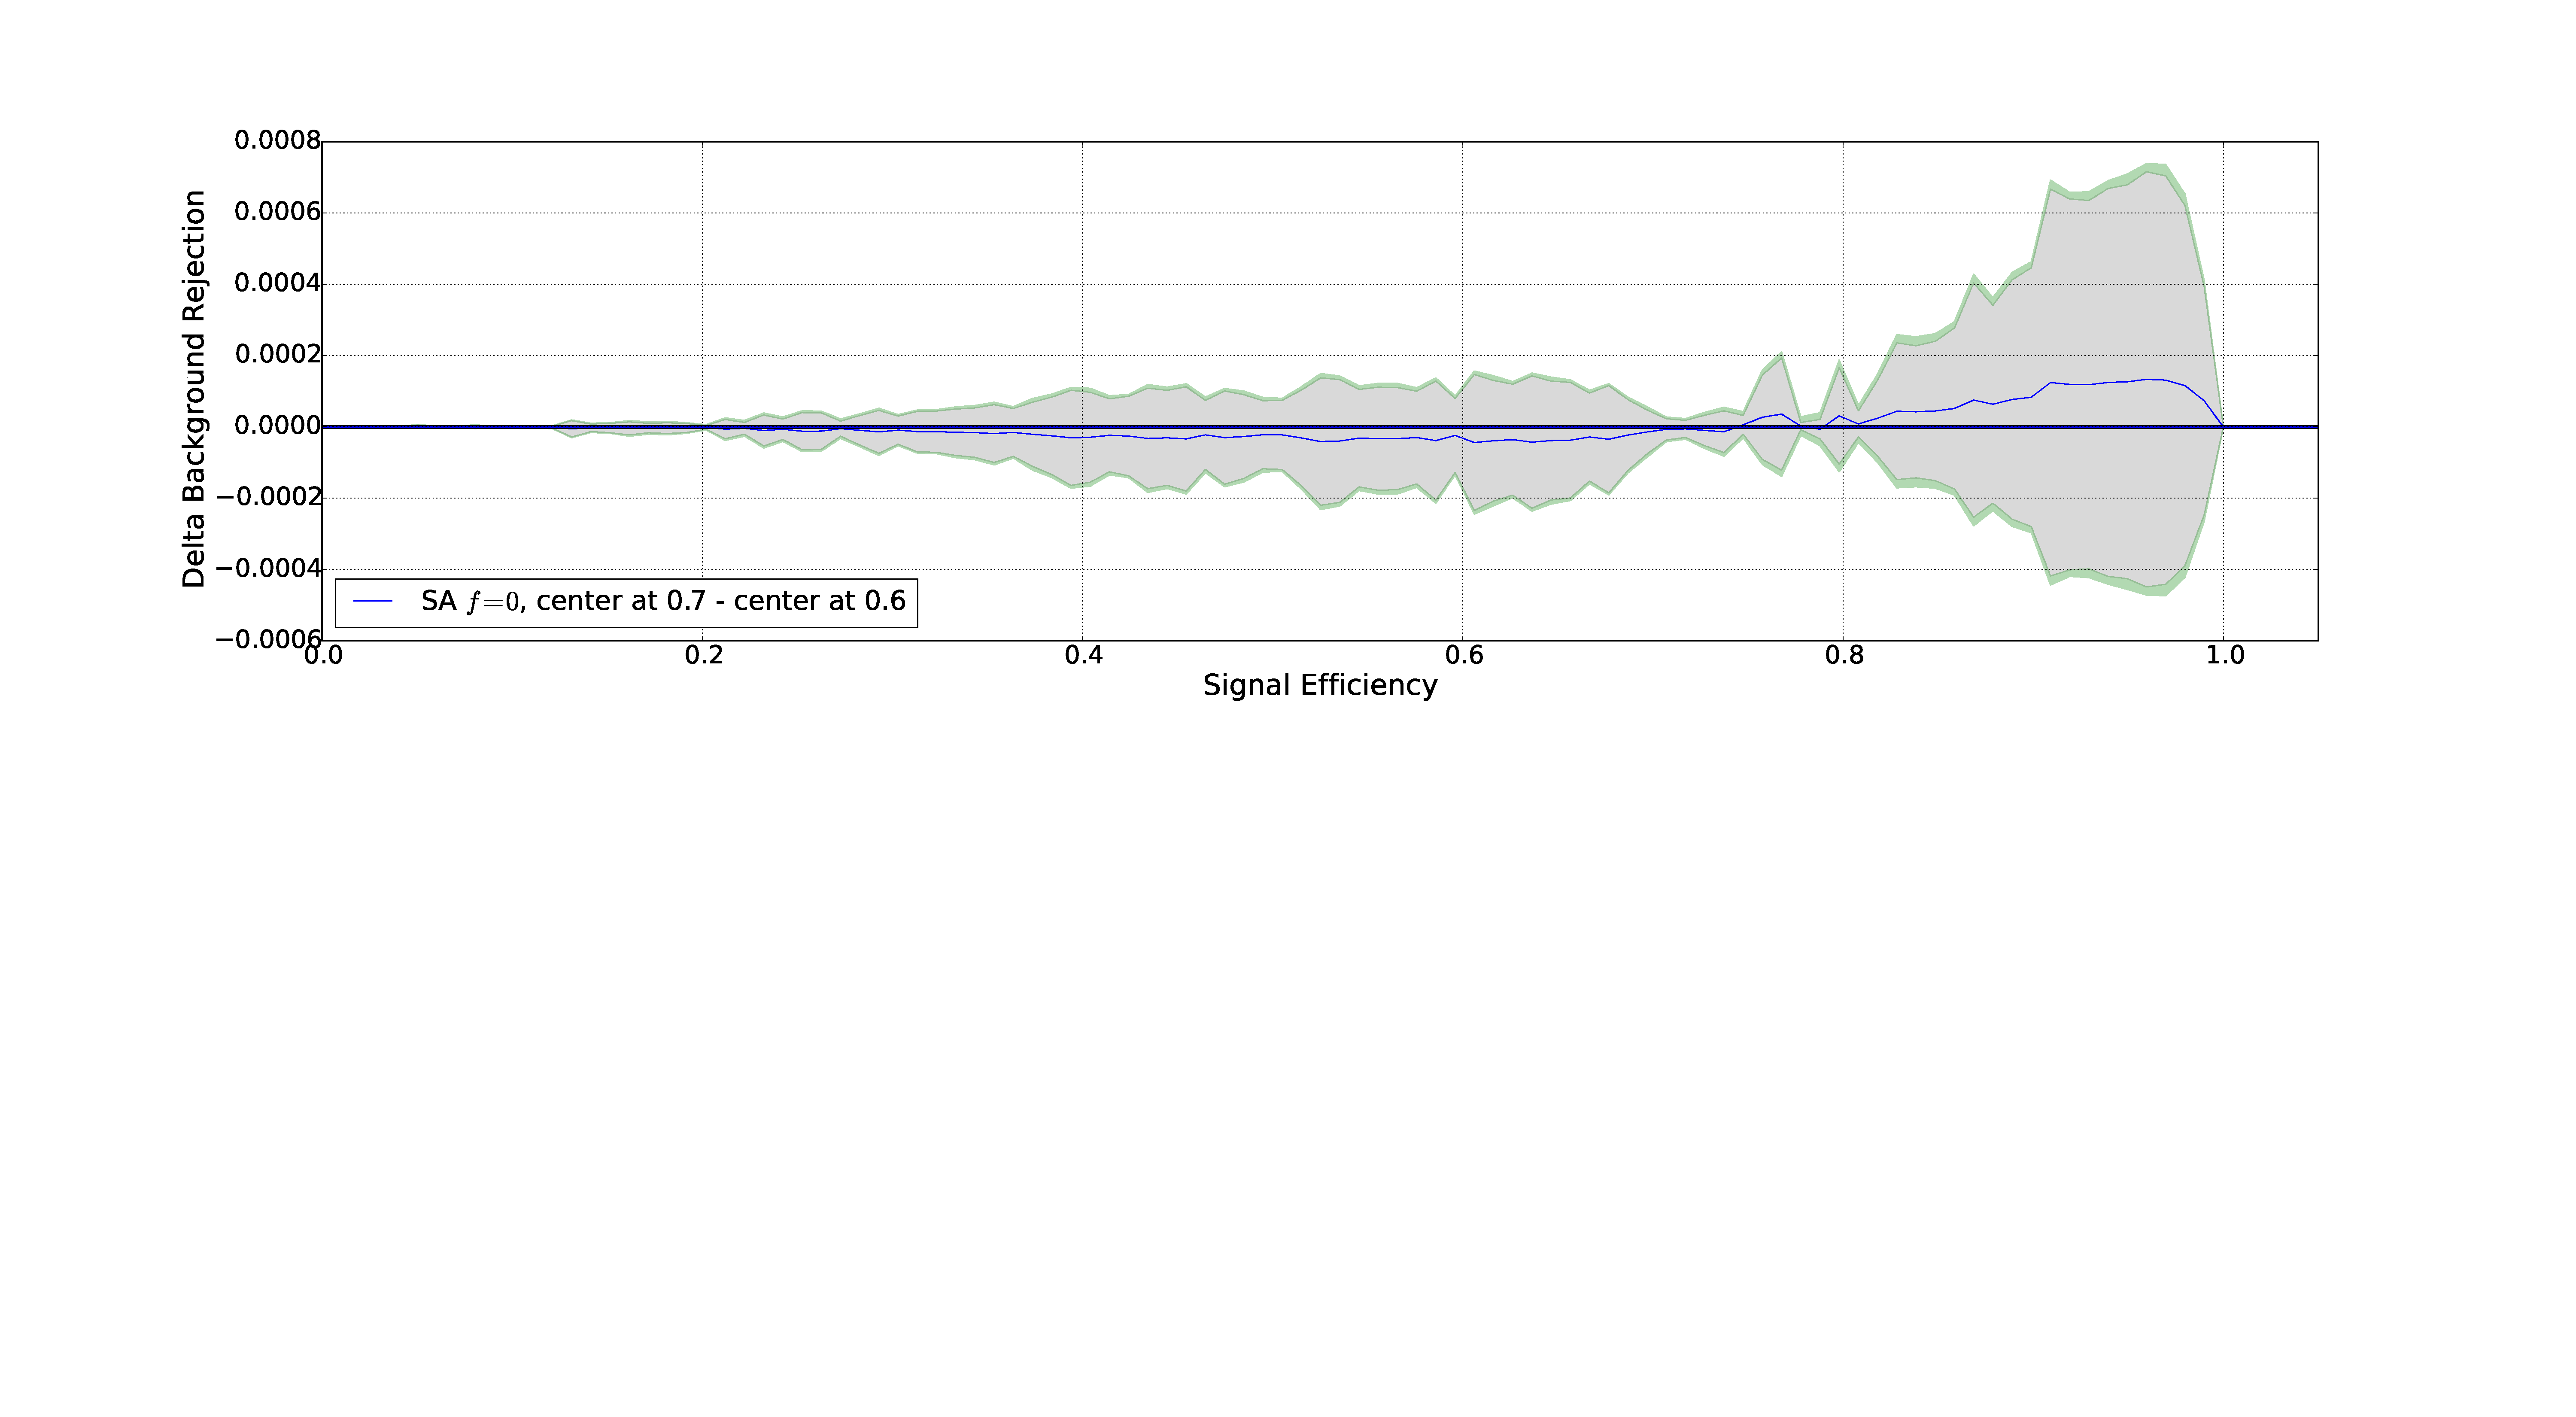
\includegraphics[width=\textwidth]{SAvc_shifted_vc_70--60_GS}\end{subfigure}
\hfill
\vspace{-5cm}
\begin{subfigure}\centering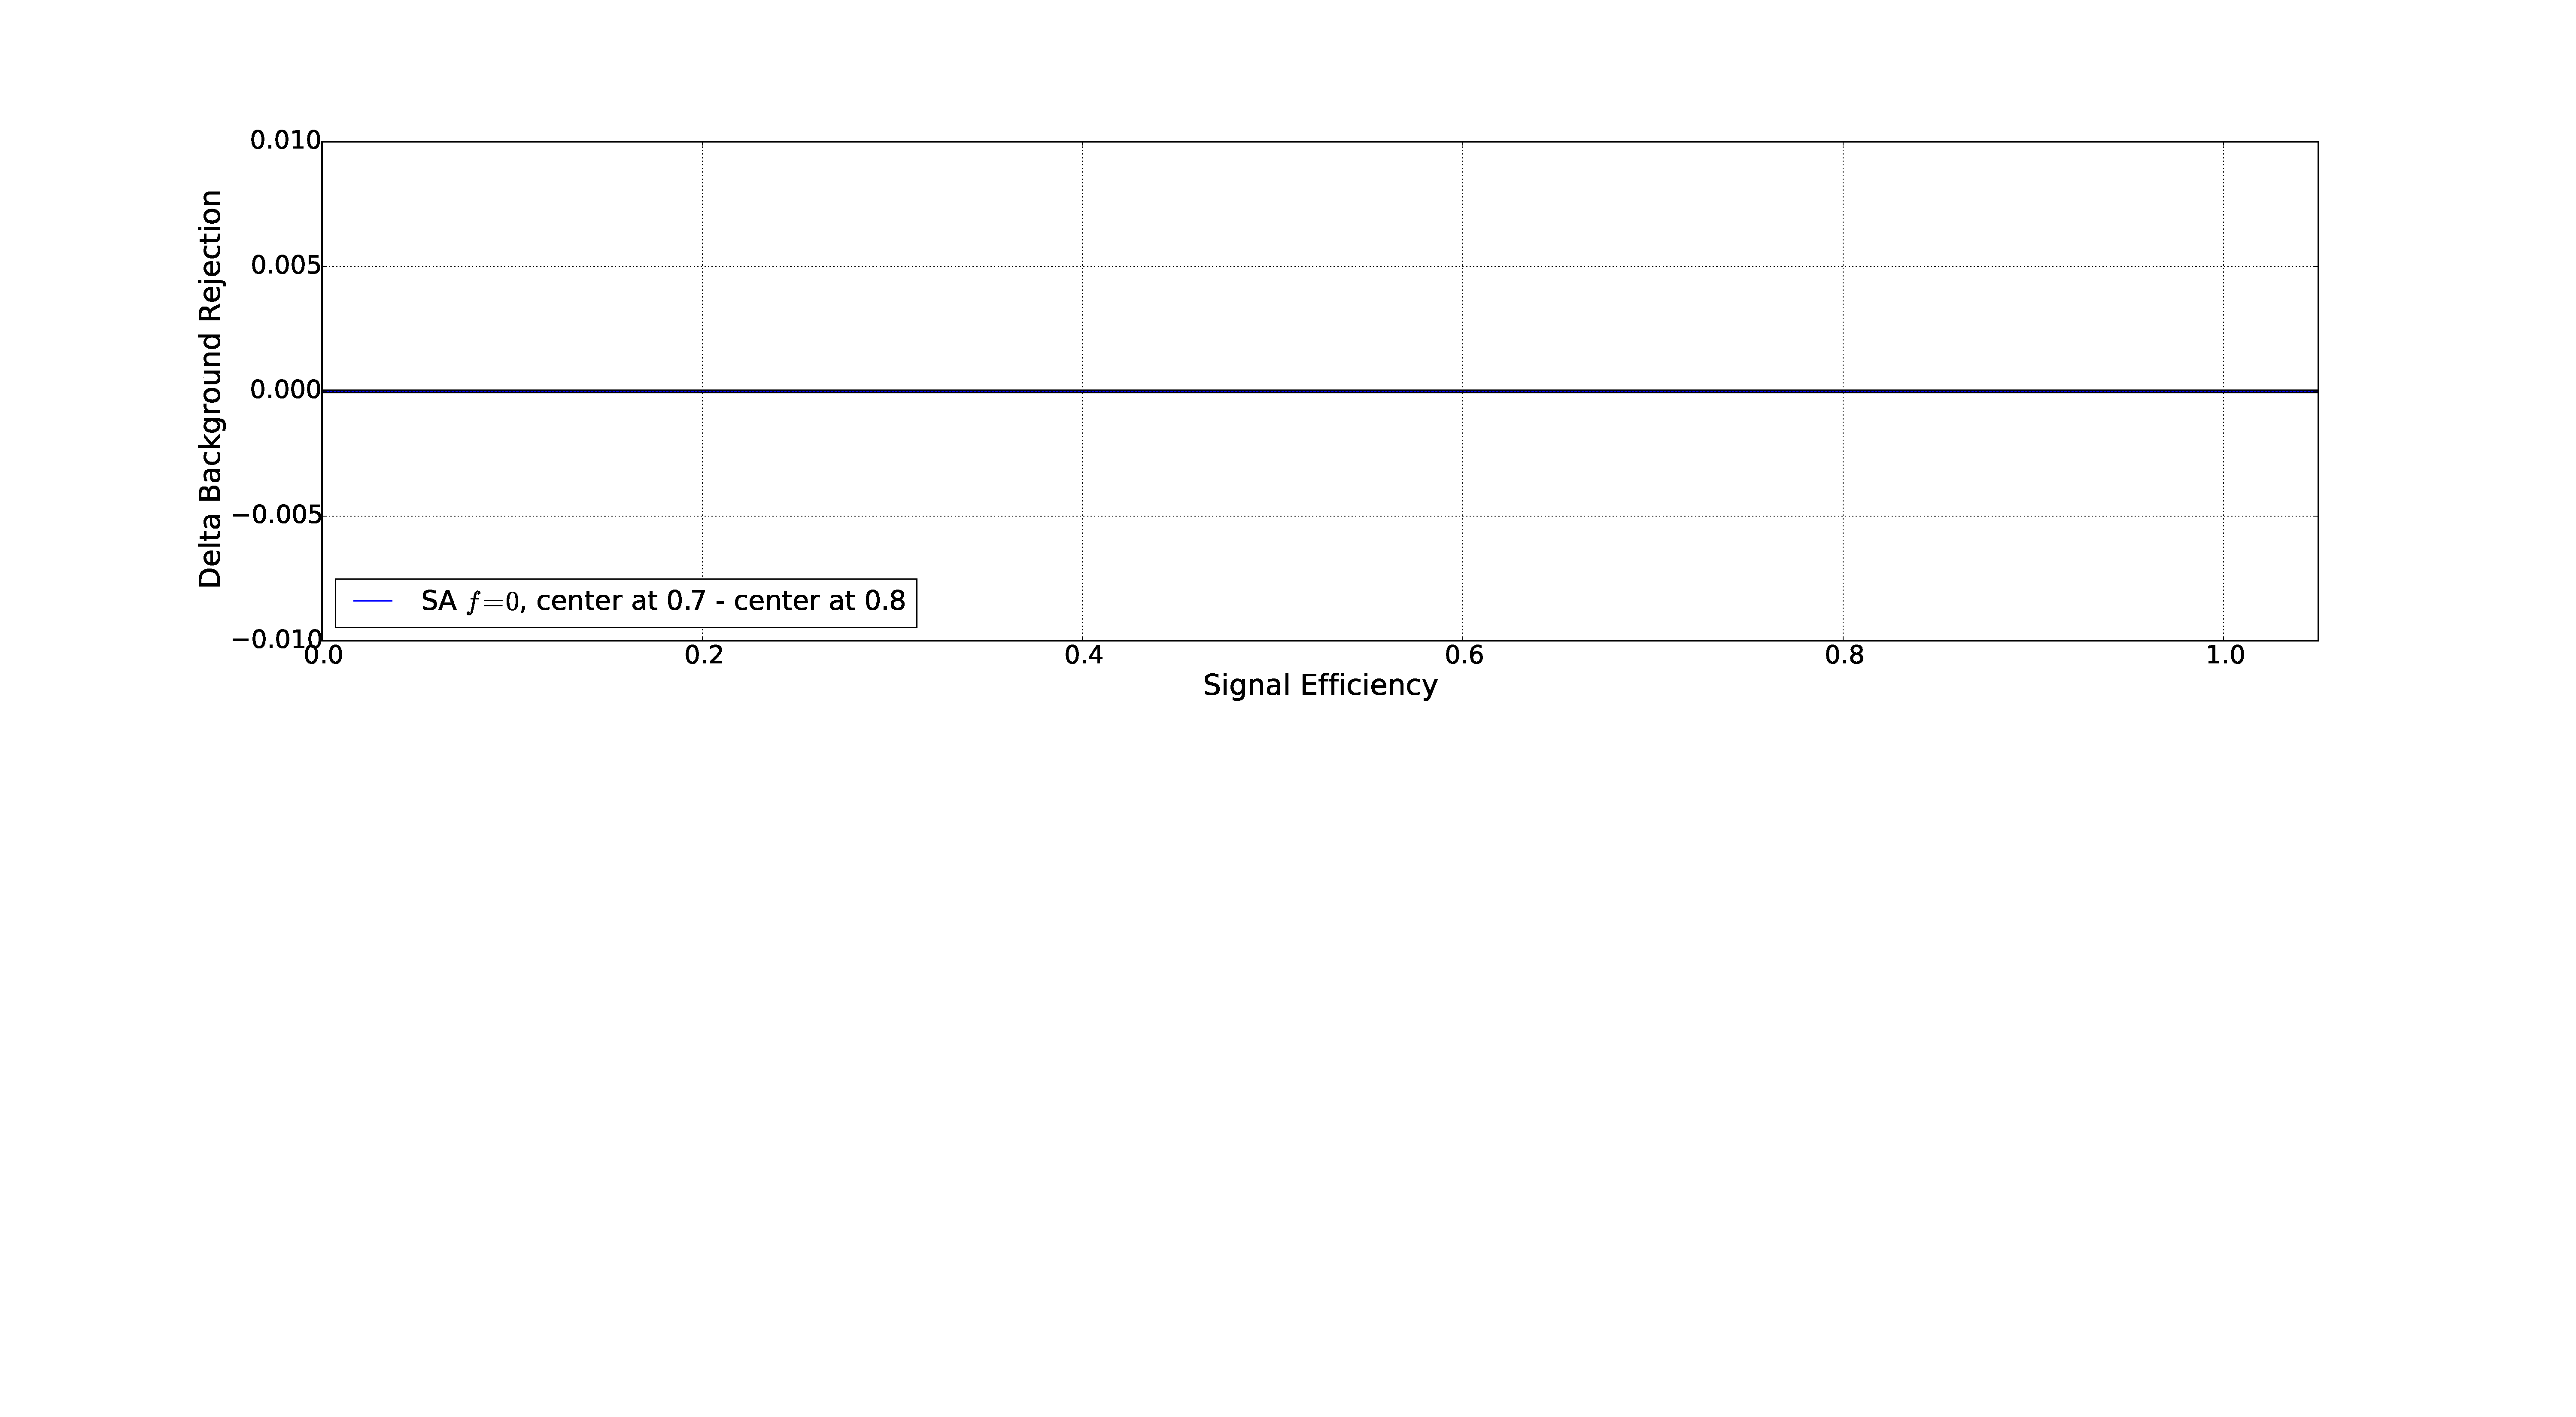
\includegraphics[width=\textwidth]{SAvc_shifted_vc_70--80_GS}\end{subfigure}
\hfill
\vspace{-5cm}
\begin{subfigure}\centering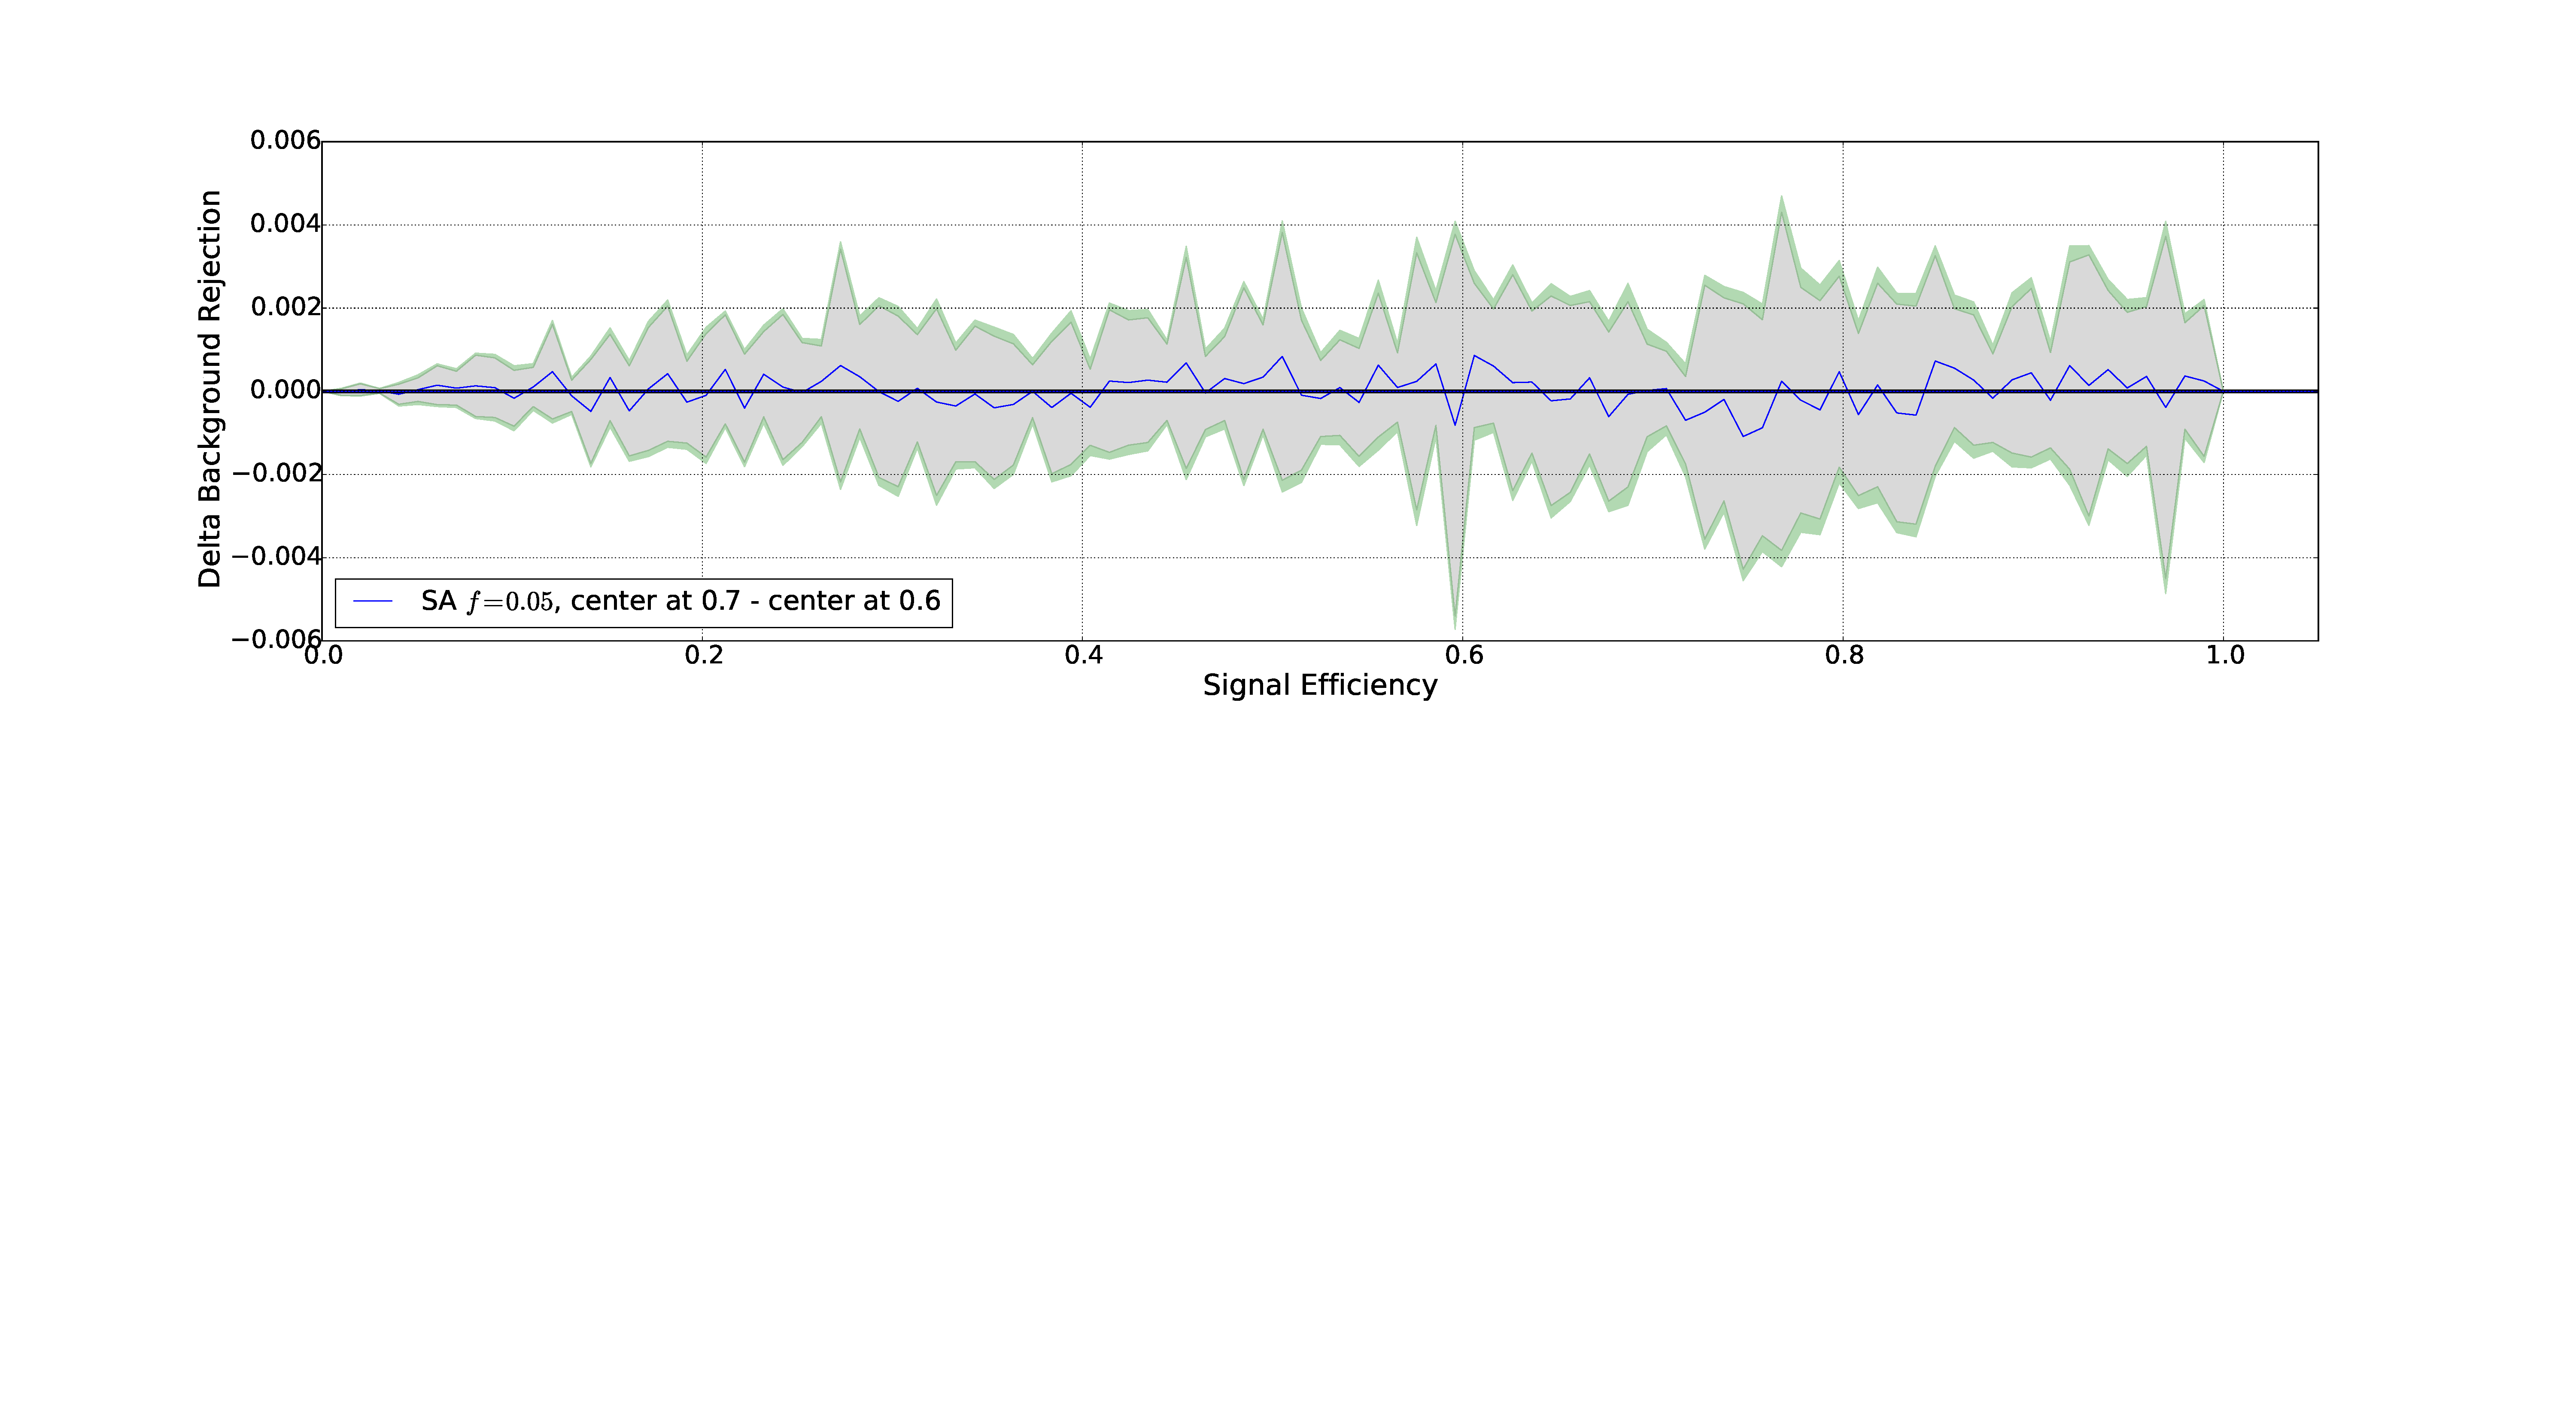
\includegraphics[width=\textwidth]{SAvc_shifted_vc_70--60_L5}\end{subfigure}
\hfill
\vspace{-5cm}
\begin{subfigure}\centering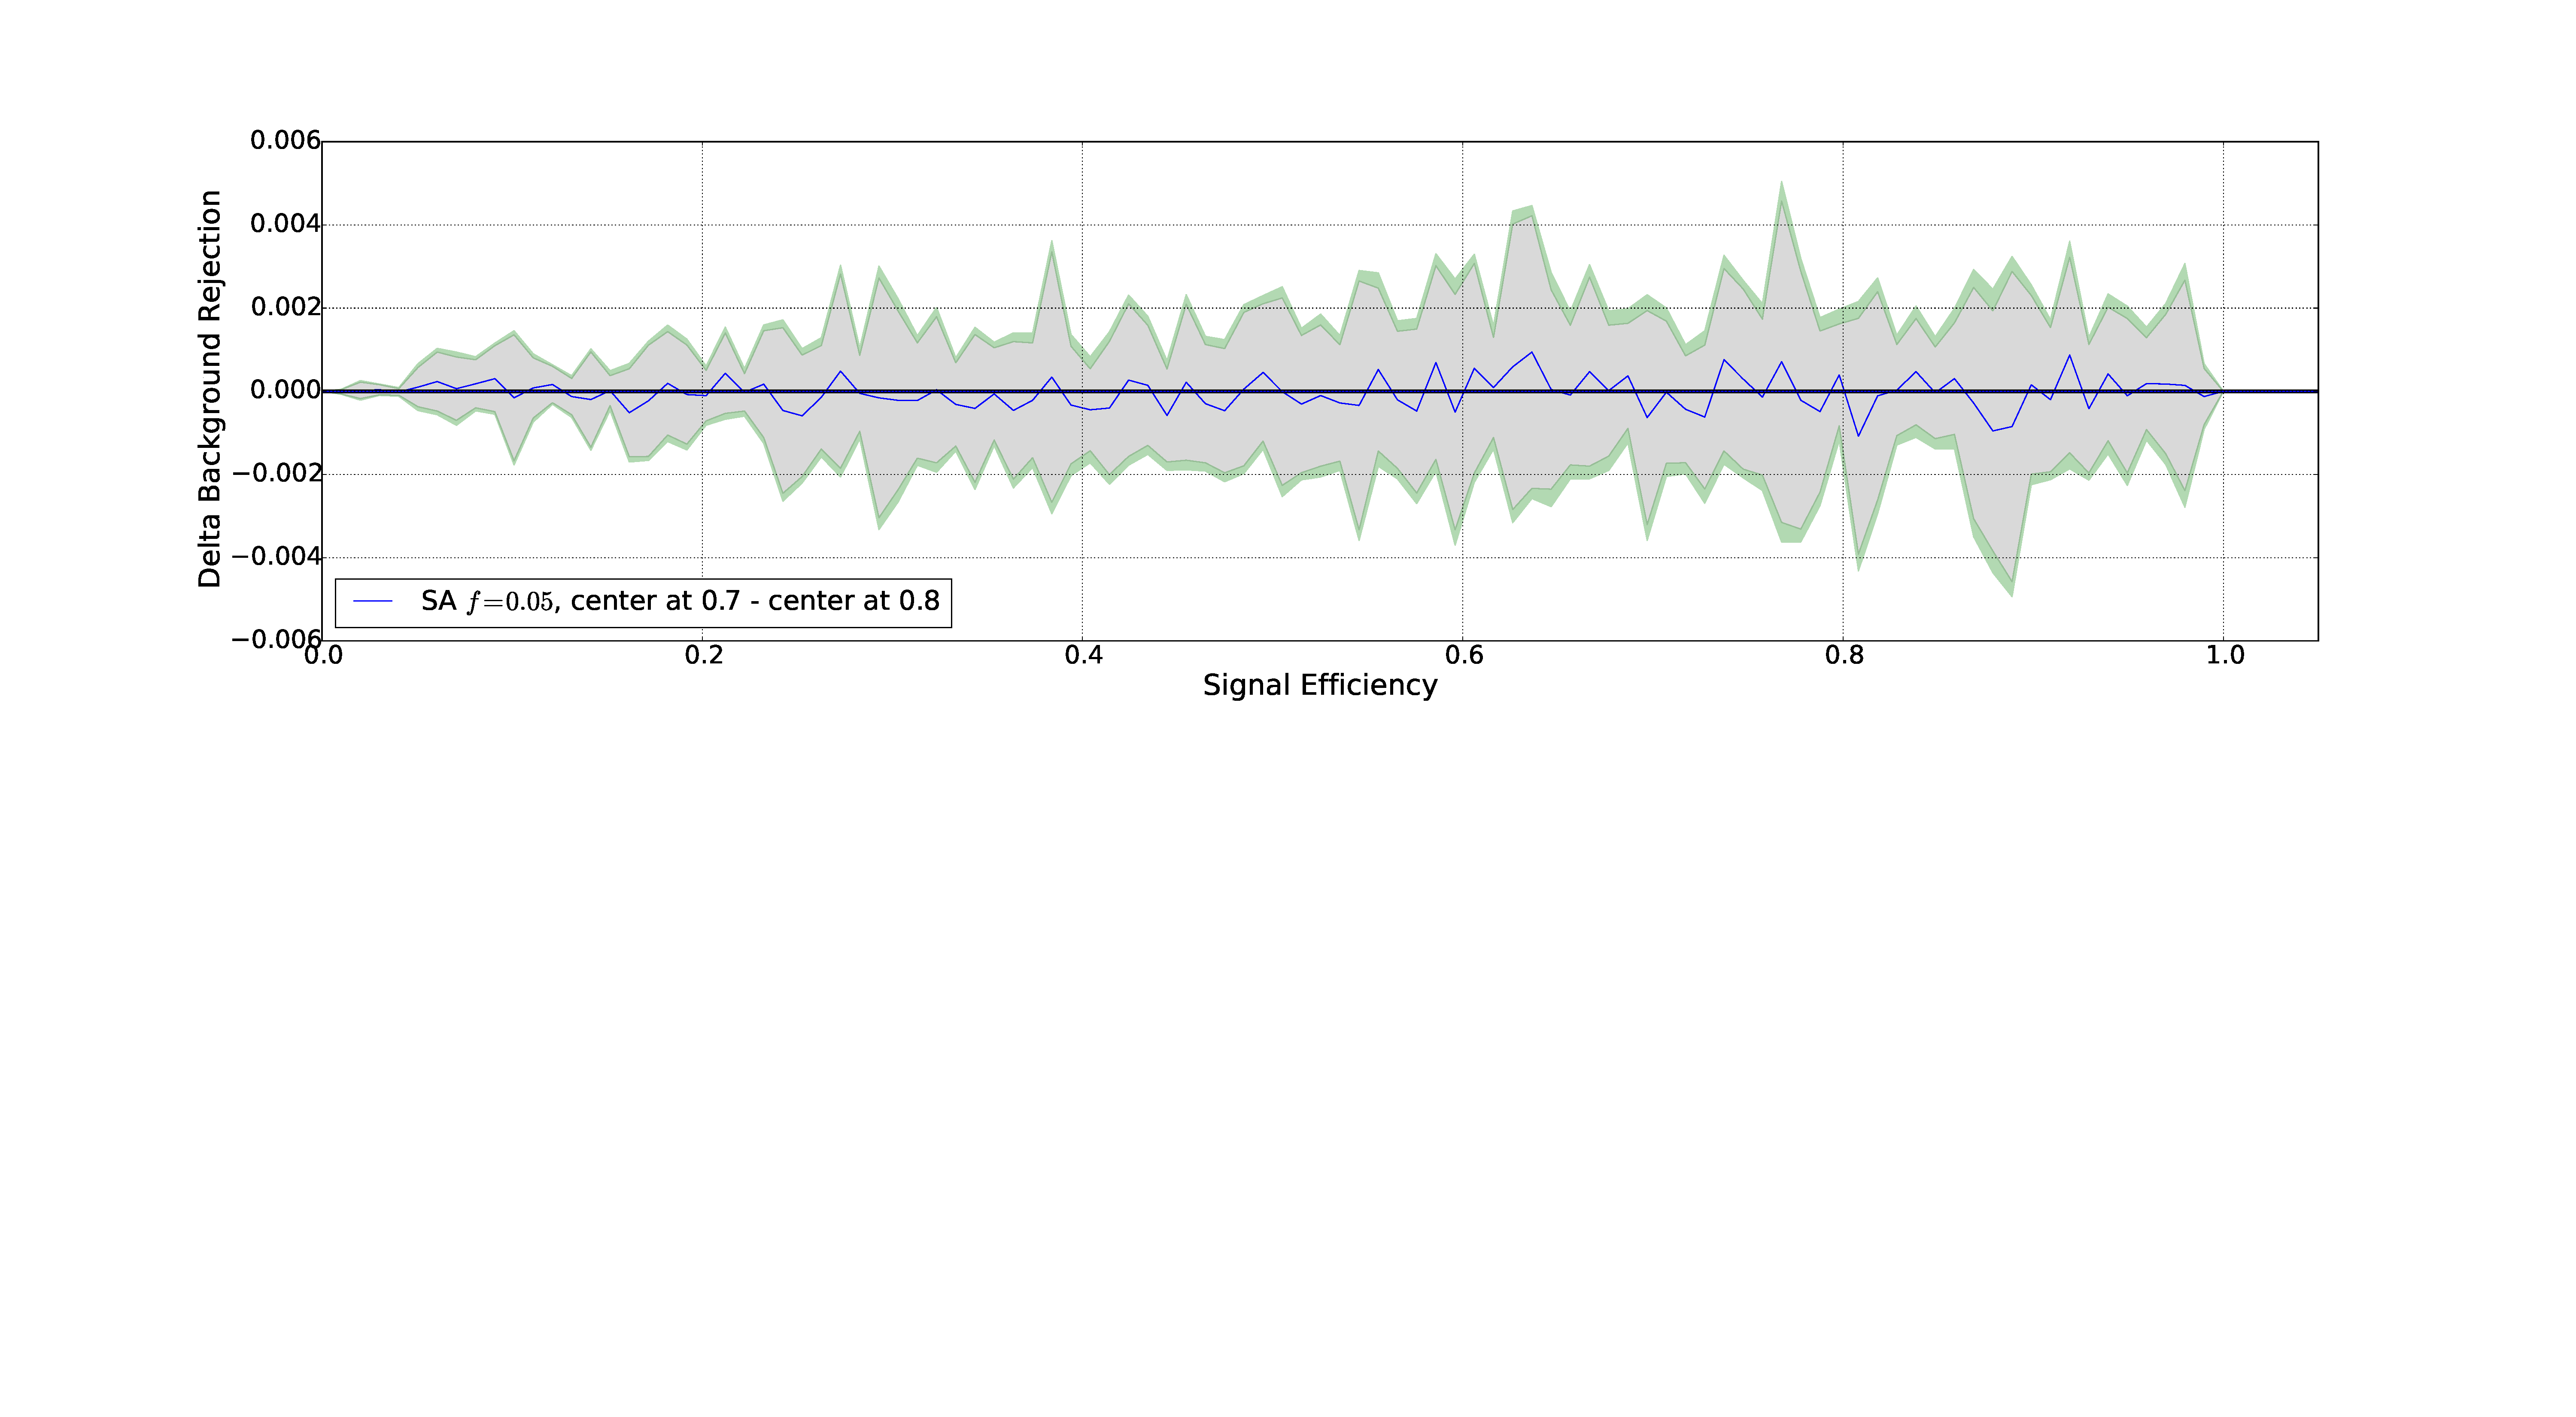
\includegraphics[width=\textwidth]{SAvc_shifted_vc_70--80_L5}\end{subfigure}
\vspace{-4cm}
\caption{Difference between the ROC curve for SA at $v_{\text{cut}}$ at the $x$th percentile during weak classifier construction and the curve using the $y$th percentile during the same for the ground state configuration. (a) $x=70$, $y=60$, $f=0$. (b) $x=70$, $y=80$, $f=0$. (c) $x=70$, $y=60$, $f=0.05$. (d) $x=70$, $y=80$, $f=0.05$.}
\label{fig:droc_vcut6070}
\end{figure}

\section*{Difference between ROC curves plots}
\label{sec:ROC-diffs}
We show differences between ROC curves for various algorithms in Figs.~\ref{fig:SA_DW_GS_droc}-\ref{fig:DW_GS_DW_L3_droc}. These form the basis for Fig.~4 in the main text, which gives the integral of the difference over signal efficiency. Figures~\ref{fig:SA_DW_GS_droc} and \ref{fig:SA_DW_L5_droc} show the difference in background rejection $r_B^{\text{DW}}-r_B^{\text{SA}}$ as a function of the signal efficiency for $f=0$ and $f=0.05$, respectively. For $f=0$ DW and SA are indistinguishable to within experimental error. For $f=0.05$ SA slightly outperforms DW in the range of low signal efficiencies for training sizes $\geq 5000$. The primary conclusion to draw from these plots is that SA differs from DW by roughly one standard deviation or less across the whole range, even though DW for training sizes larger than $100$ struggles to find states within less than $5\%$ of the ground state energy. This suggests a robustness of QAML, 
which (if it generalizes to other problems) significantly improves the potential to exploit physical quantum annealers to solve machine learning problems and achieve close-to-optimal classifier performance, even in the presence of significant processor noise.

Figures~\ref{fig:SA_DNN_GS_droc} and \ref{fig:SA_XGB_GS_droc} show the ROC difference between DW and DNN and DW and XGB at $f=0$, respectively. The two cases have broadly similar shapes. One clearly sees that QAML on DW outperforms DNN and XGB at the smallest training size in a statistically significant manner, but that the trend reverses for sizes $\geq 5000$. Note, that at the scale of these diagrams, the gap between $f=0$ and $f=0.05$ is negligible.

Figures~\ref{fig:SA_GS_SA_L3_droc} (SA) and \ref{fig:DW_GS_DW_L3_droc} (DW) show the difference between $f=0$ and $f=0.05$. SA and DW exhibit broadly similar behavior, with an improvement with excited states of $\approx 0.4\%$ in background rejection for SA and of $\approx 0.2\%$ for DW. The improvement increases with training size and is slightly larger for SA than DW (though this difference is likely simply noise, as it is less than half the standard deviation of each distribution). It should be noted that since QAML's comparative advantage against other techniques appears to be in the realm of small training sizes. However, this is the same range where including excited states has no benefit.


\begin{figure}[h]
\centering
% \begin{adjustbox}{center}
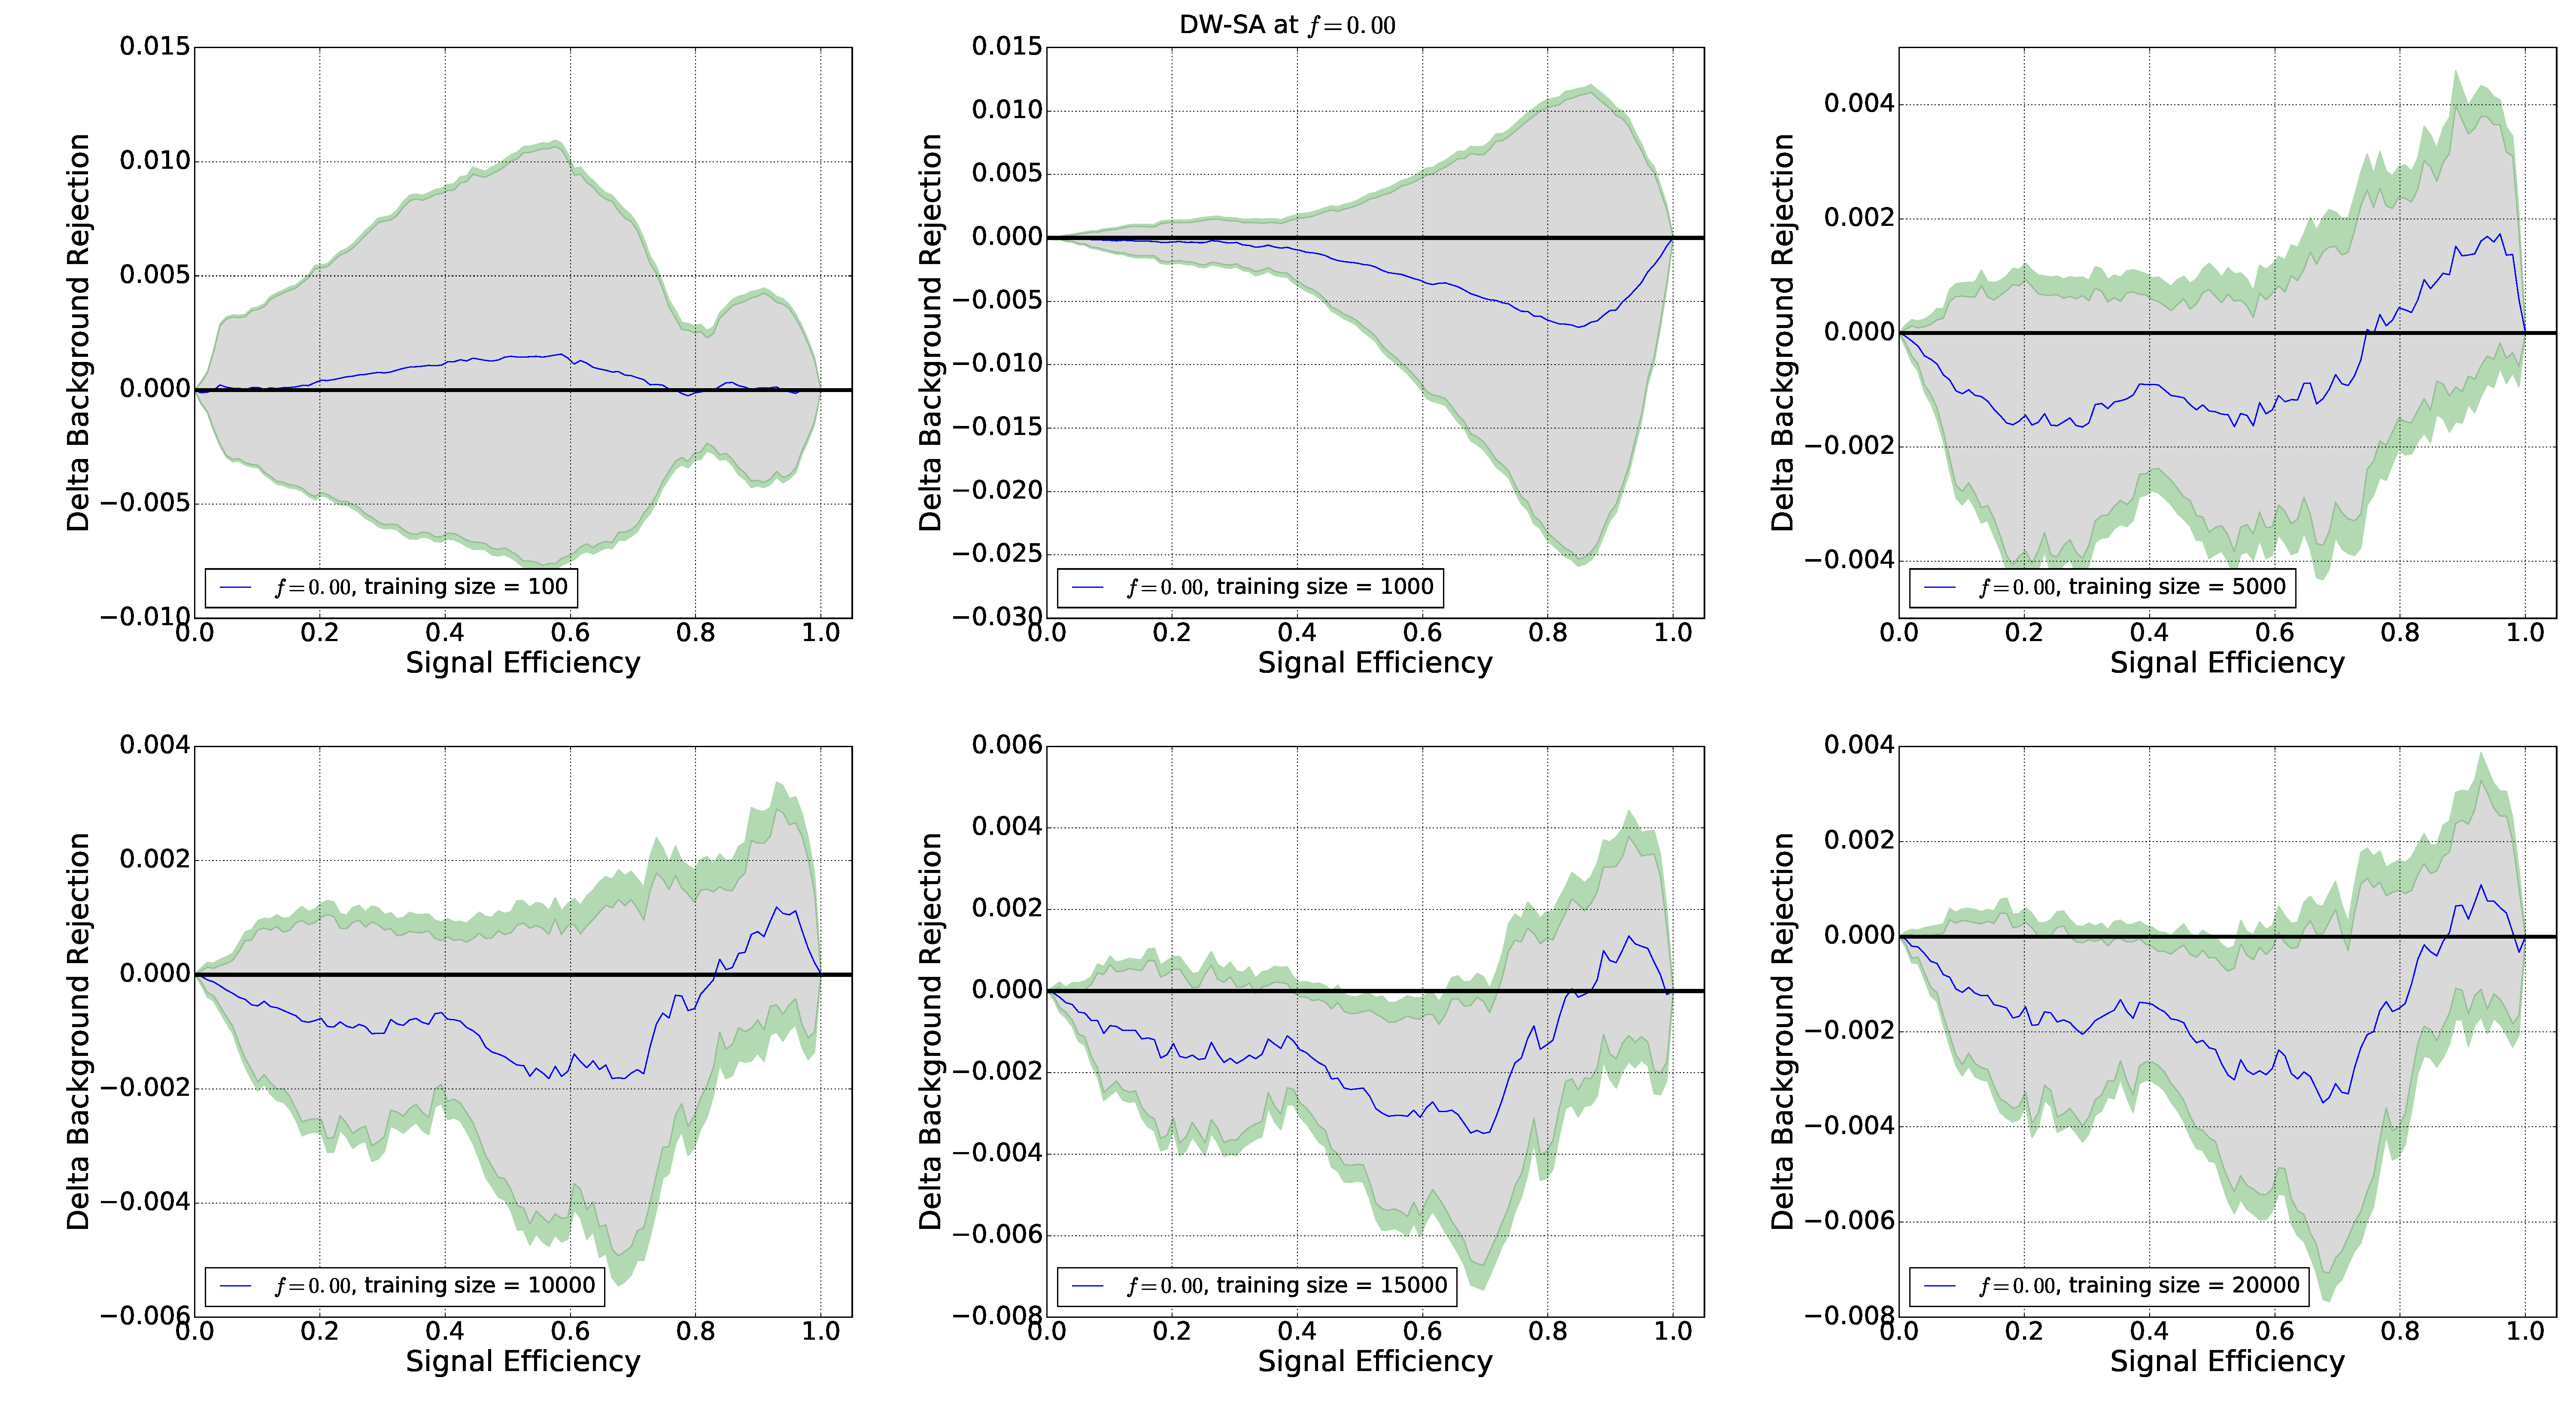
\includegraphics[width=0.8\paperwidth]{DW--SA_GS}
% \end{adjustbox}
\caption{Difference between the ROC curves for SA and DW using the minimum energy returned.}
\label{fig:SA_DW_GS_droc}
\end{figure}

\begin{figure}[h]
\centering
% \begin{adjustbox}{center}
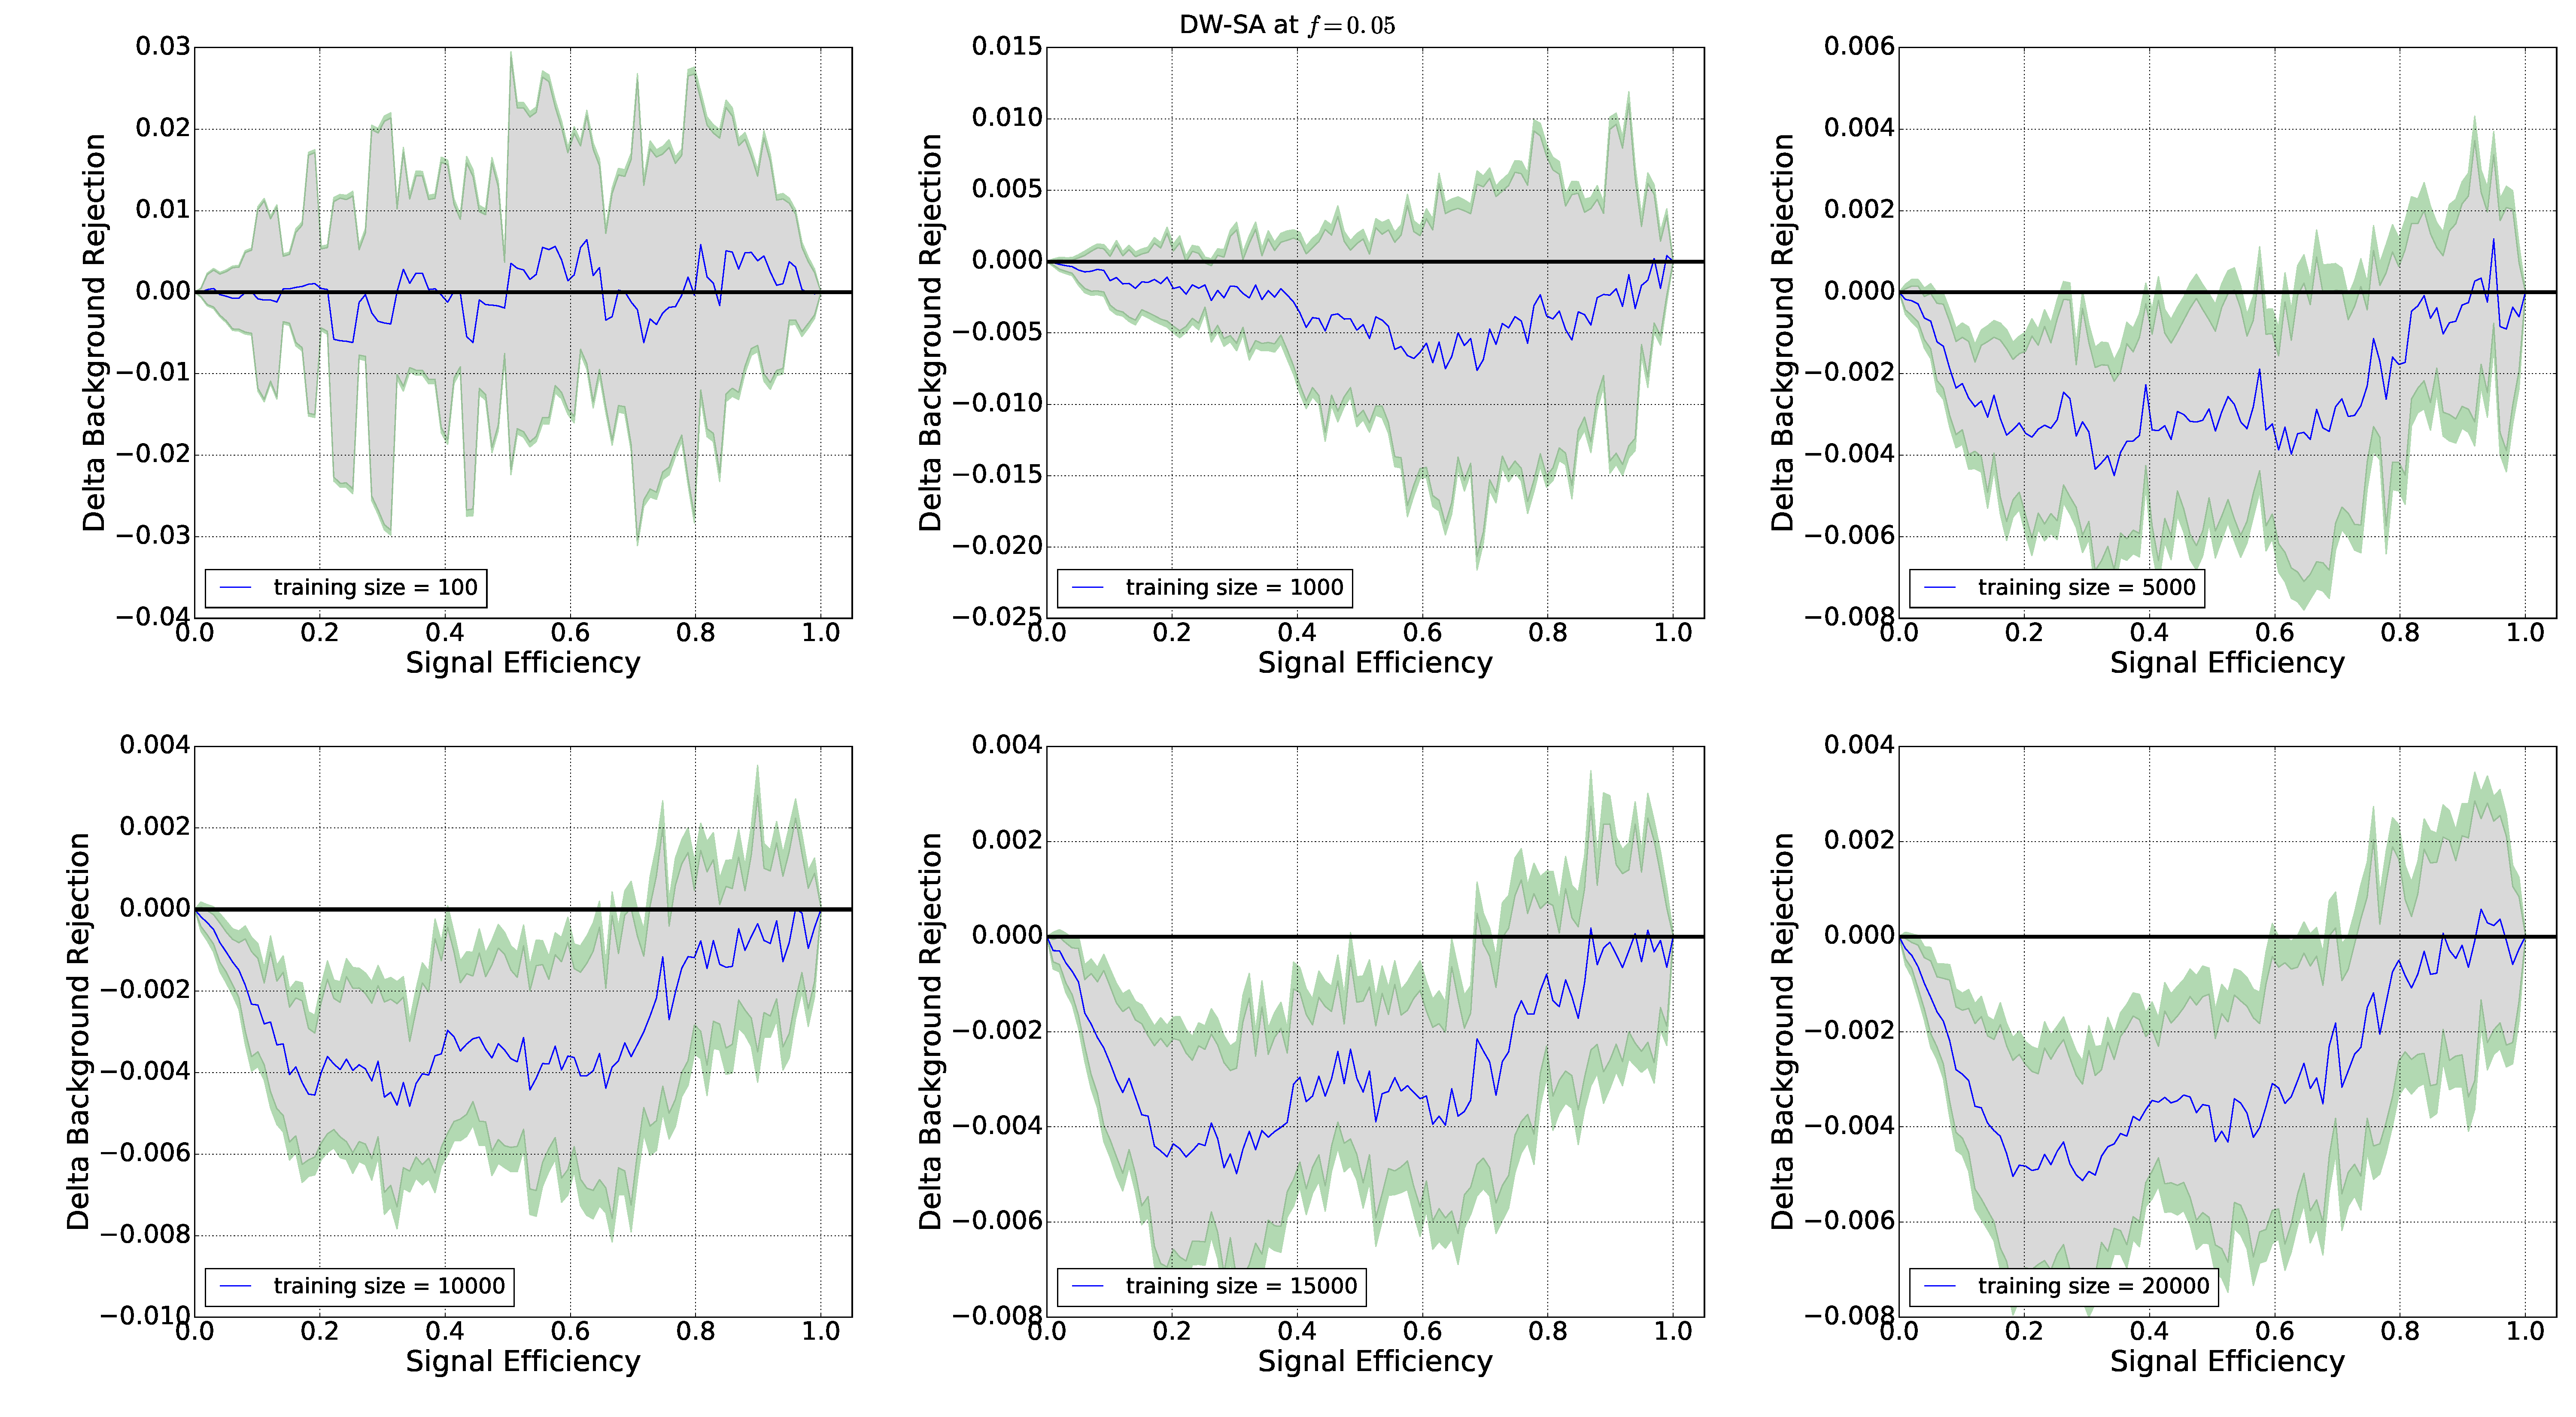
\includegraphics[width=0.8\paperwidth]{DW--SA_L5}
% \end{adjustbox}
\caption{Difference between the ROC curves for SA and DW using all states within $5\%$ of the minimum return energy.}
\label{fig:SA_DW_L5_droc}
\end{figure}
\begin{figure}[h]
\centering
% \begin{adjustbox}{center}
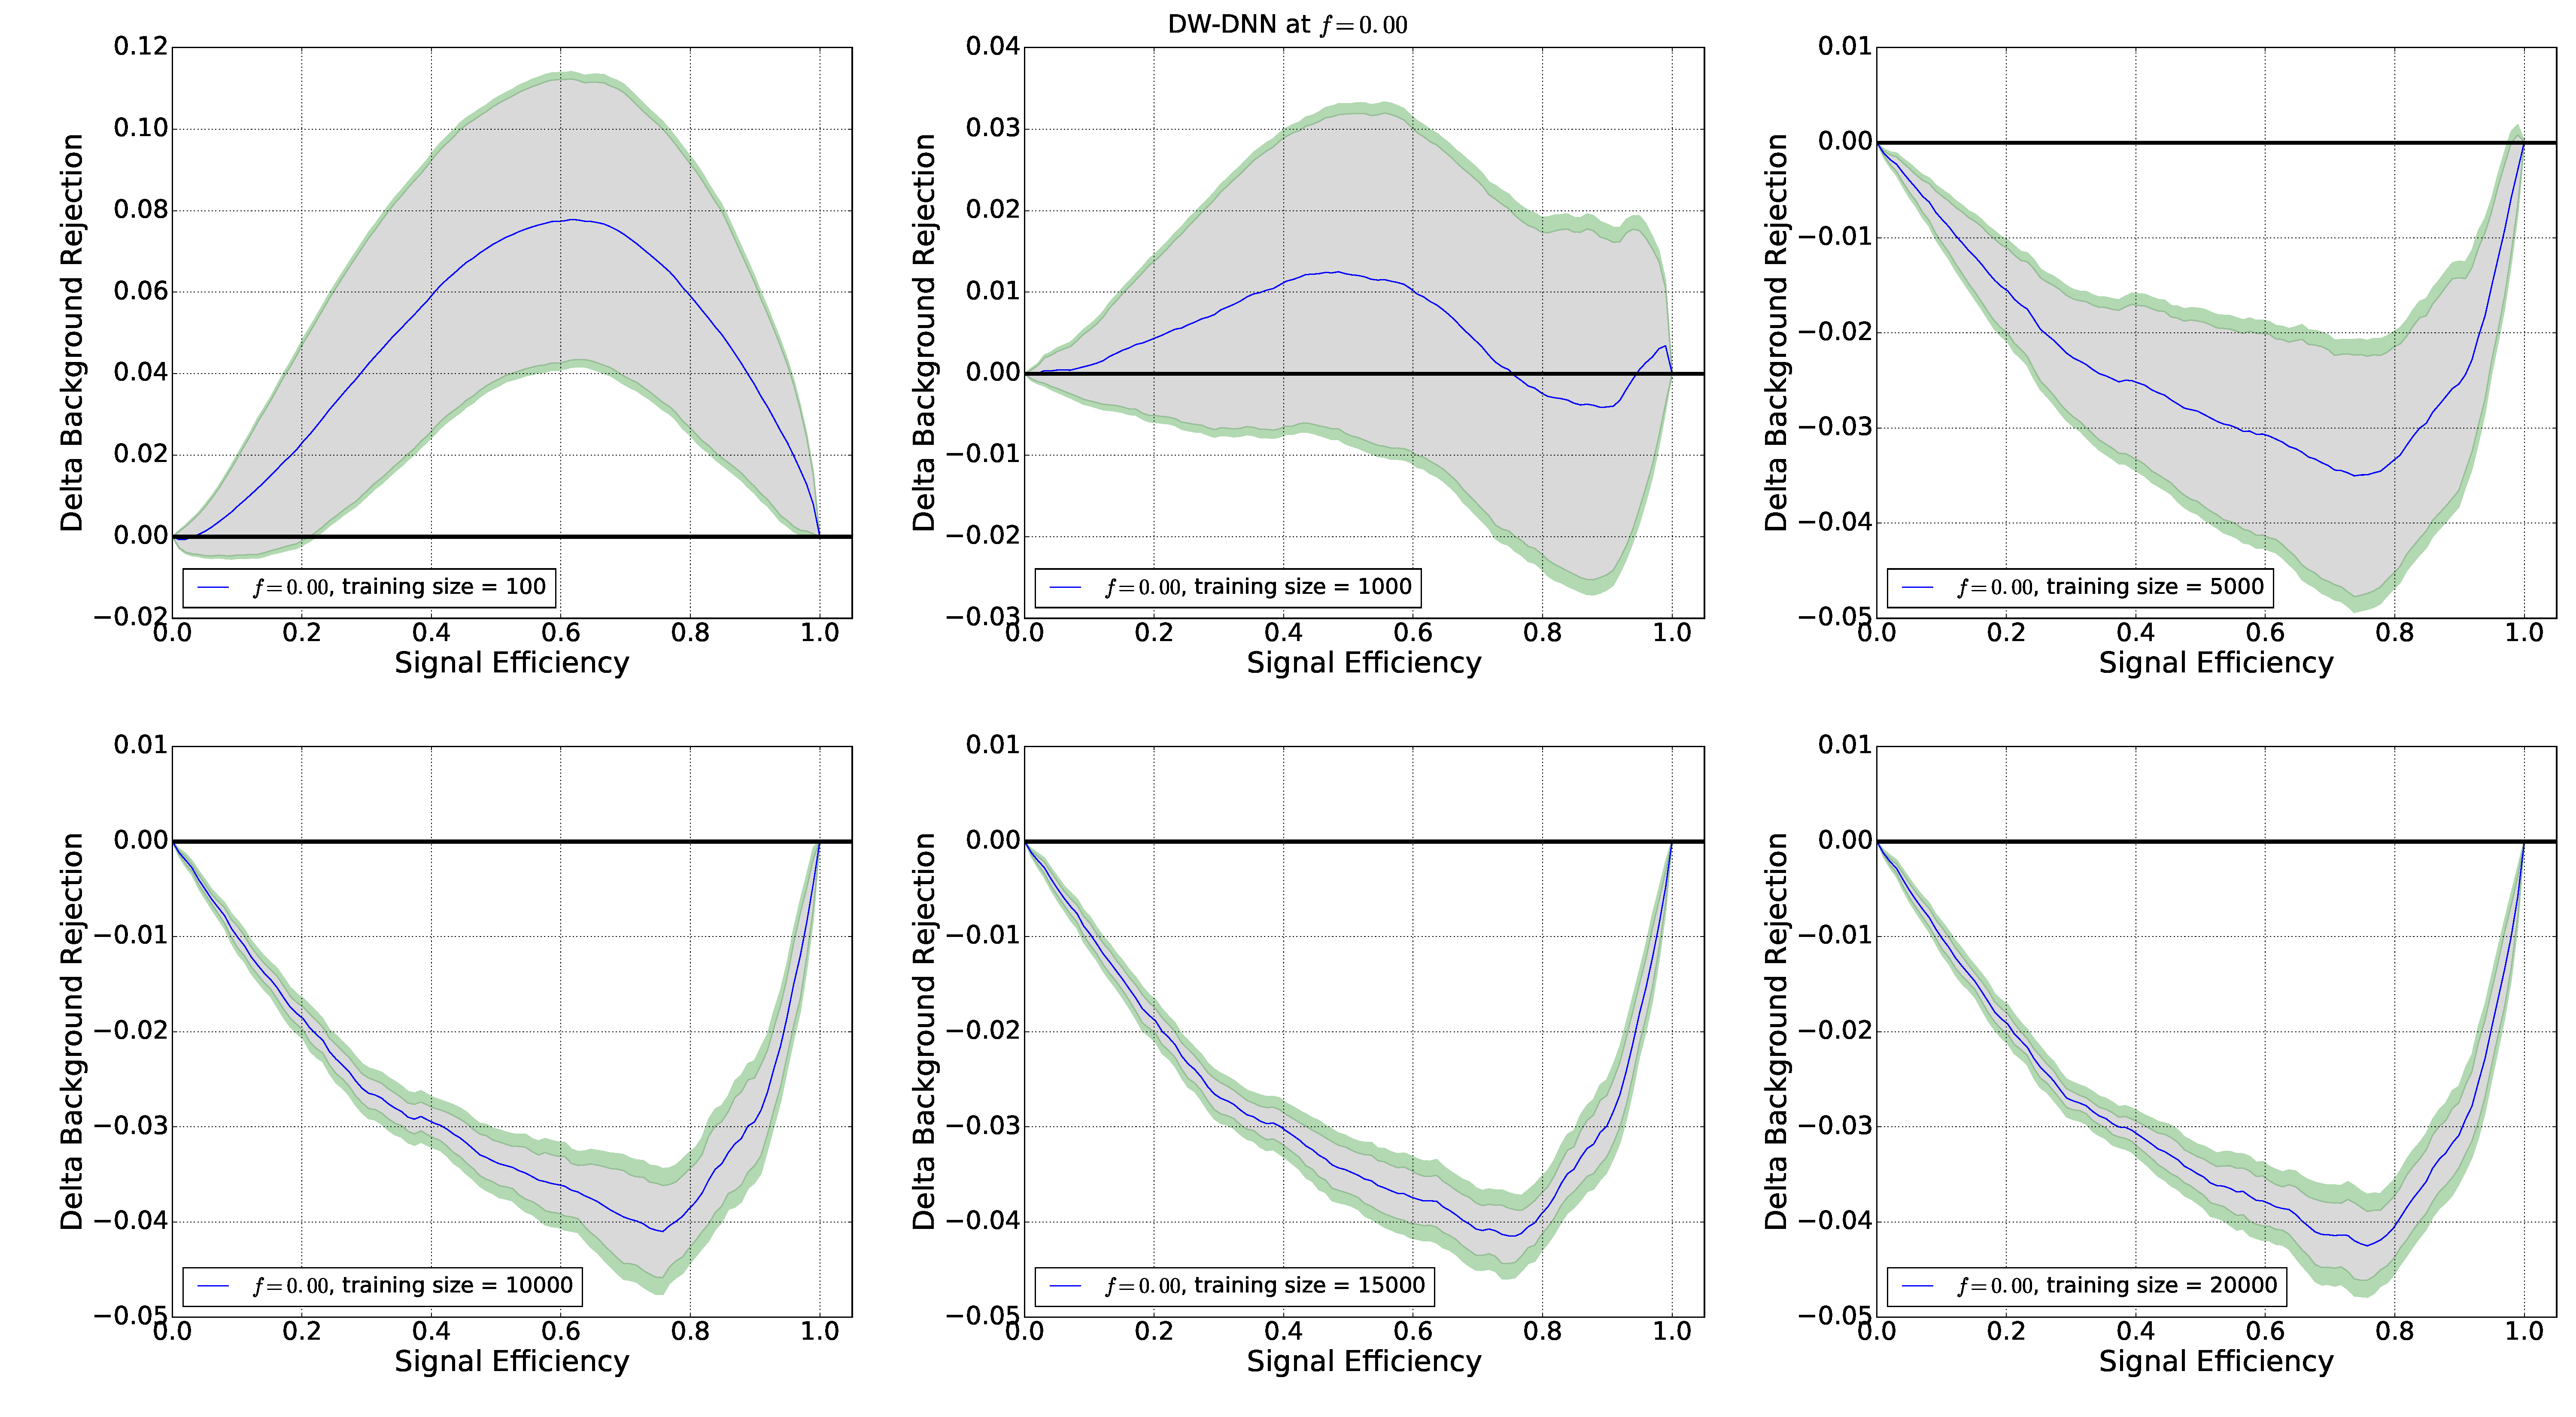
\includegraphics[width=0.8\paperwidth]{DW--DNN_GS}
% \end{adjustbox}
\caption{Difference between the ROC curves for DW and DNN using the minimum energy configuration from DW.}
\label{fig:SA_DNN_GS_droc}
\end{figure} 

\begin{figure}[h]
\centering
% \begin{adjustbox}{center}
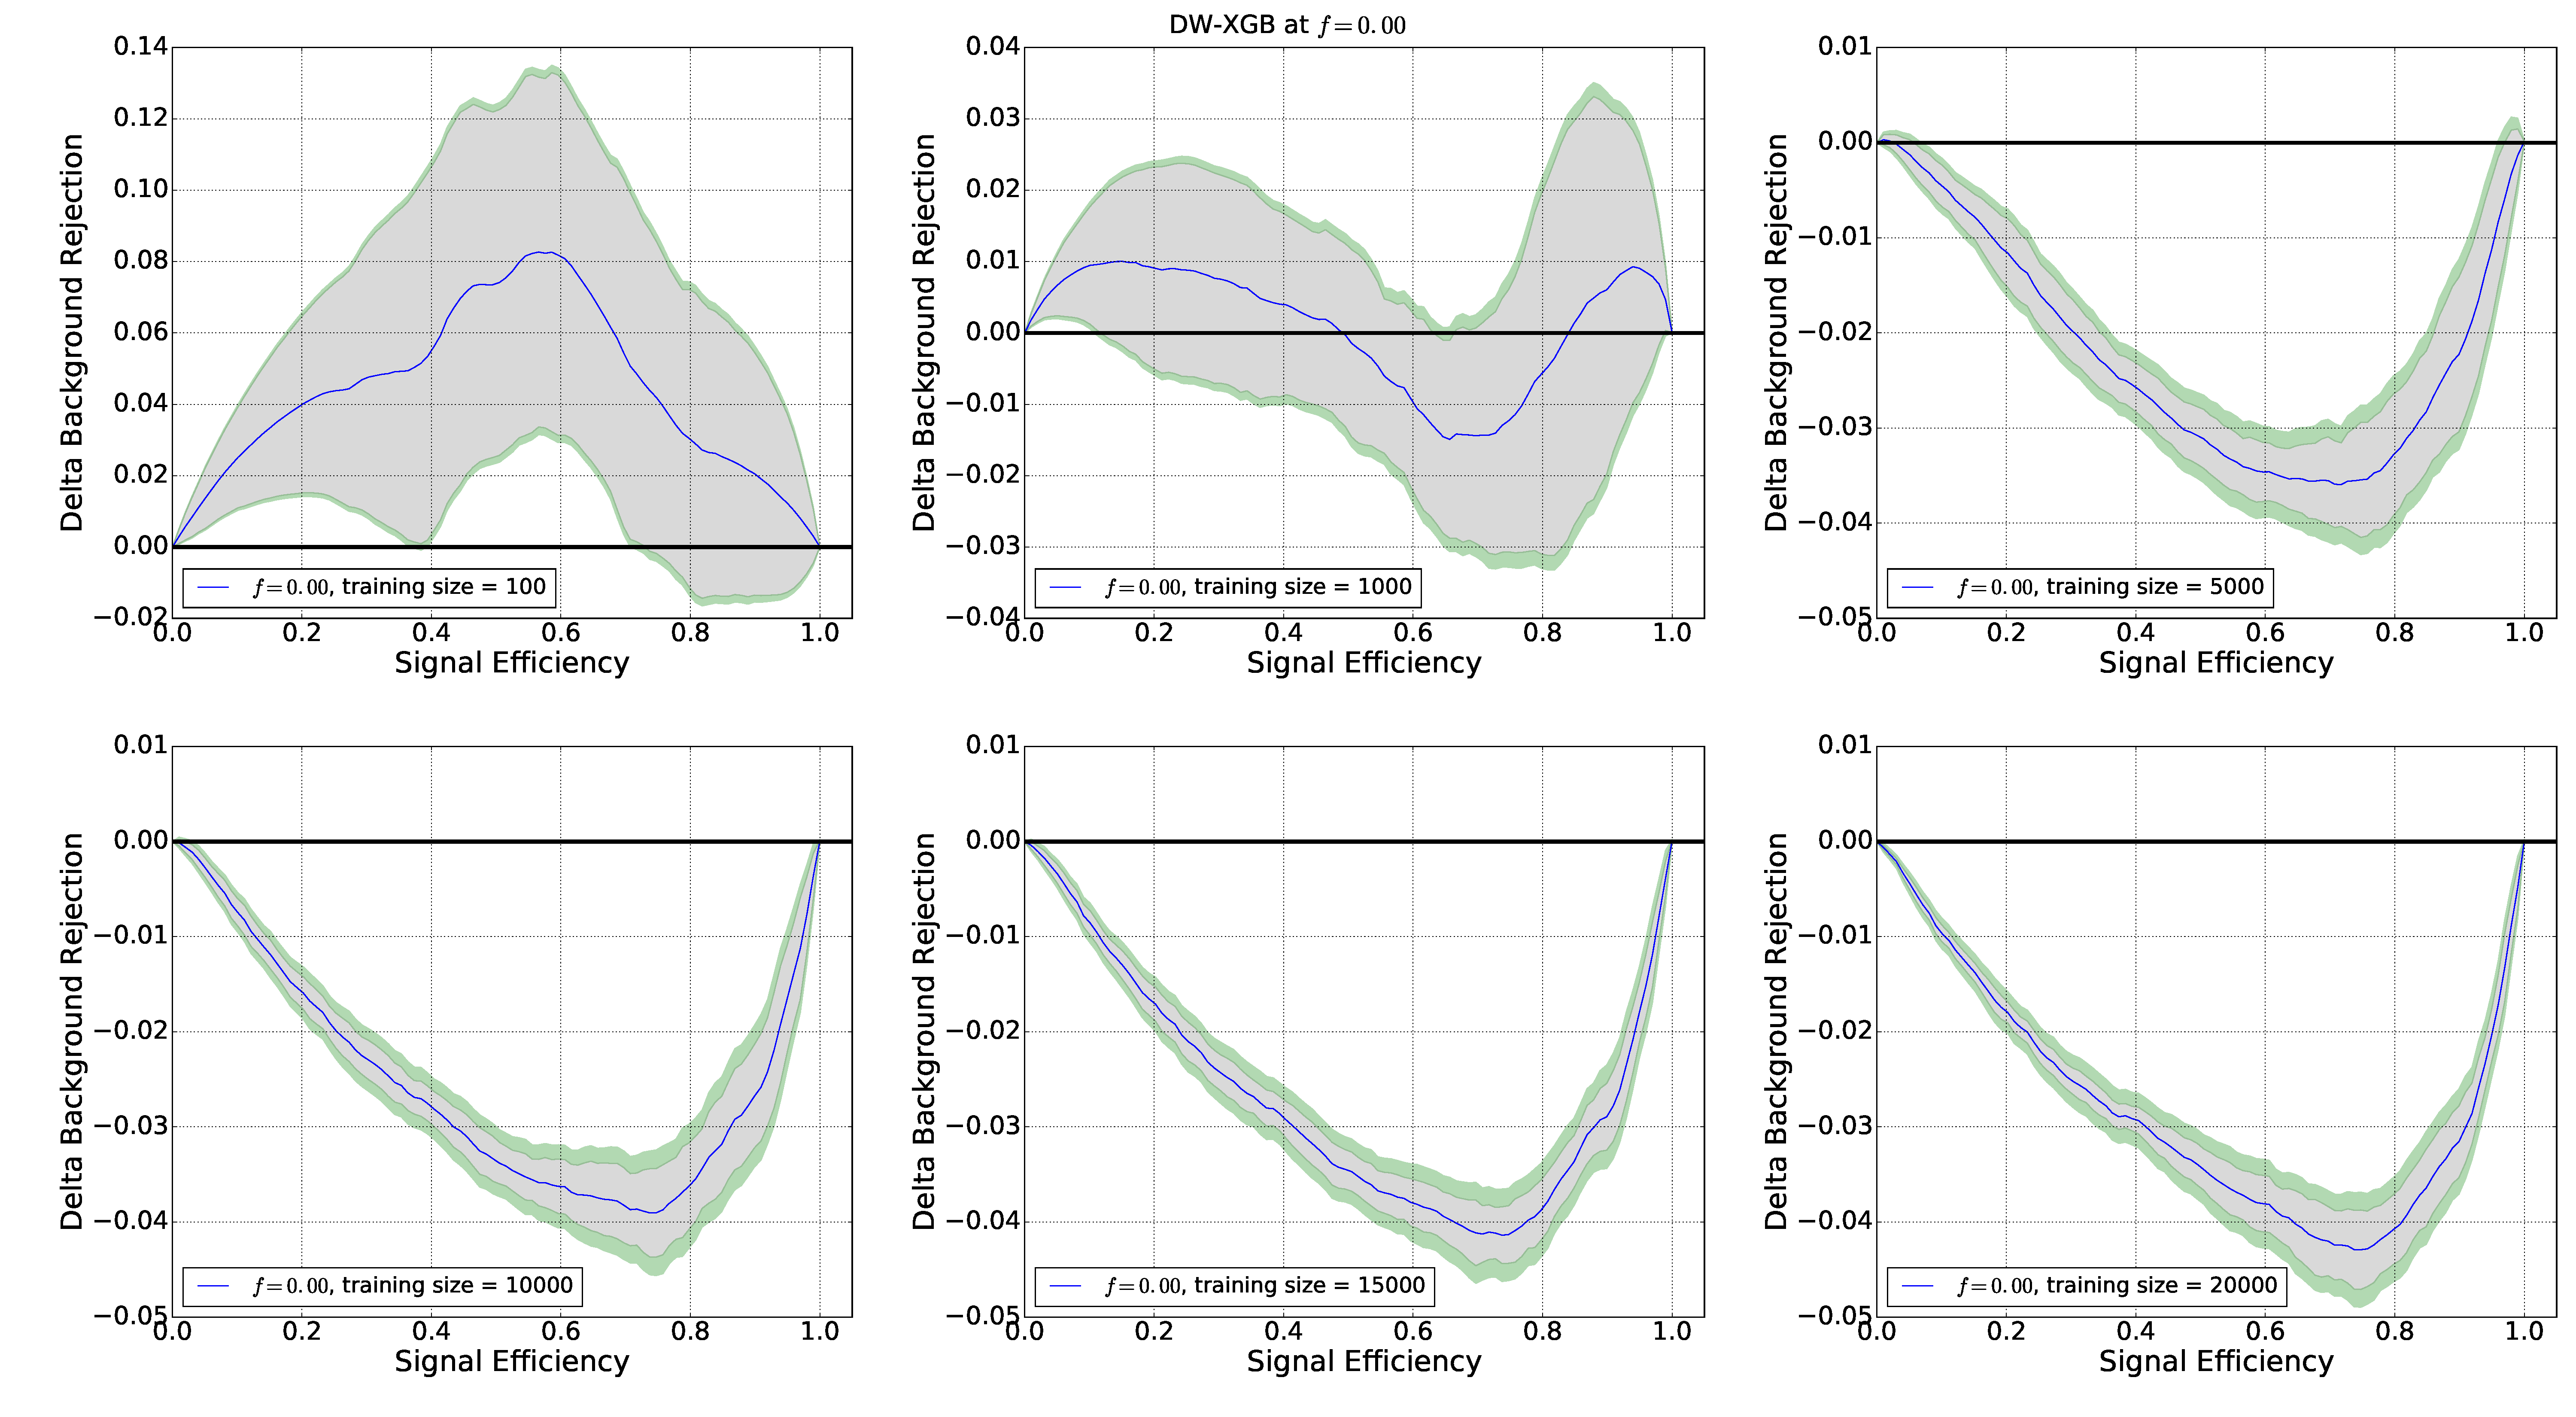
\includegraphics[width=0.8\paperwidth]{DW--XGB_GS}
% \end{adjustbox}
\caption{Difference between the ROC curves for DW and XGB using the minimum energy configuration from DW.}
\label{fig:SA_XGB_GS_droc}
\end{figure}

\begin{figure}[h]
\centering
% \begin{adjustbox}{center}
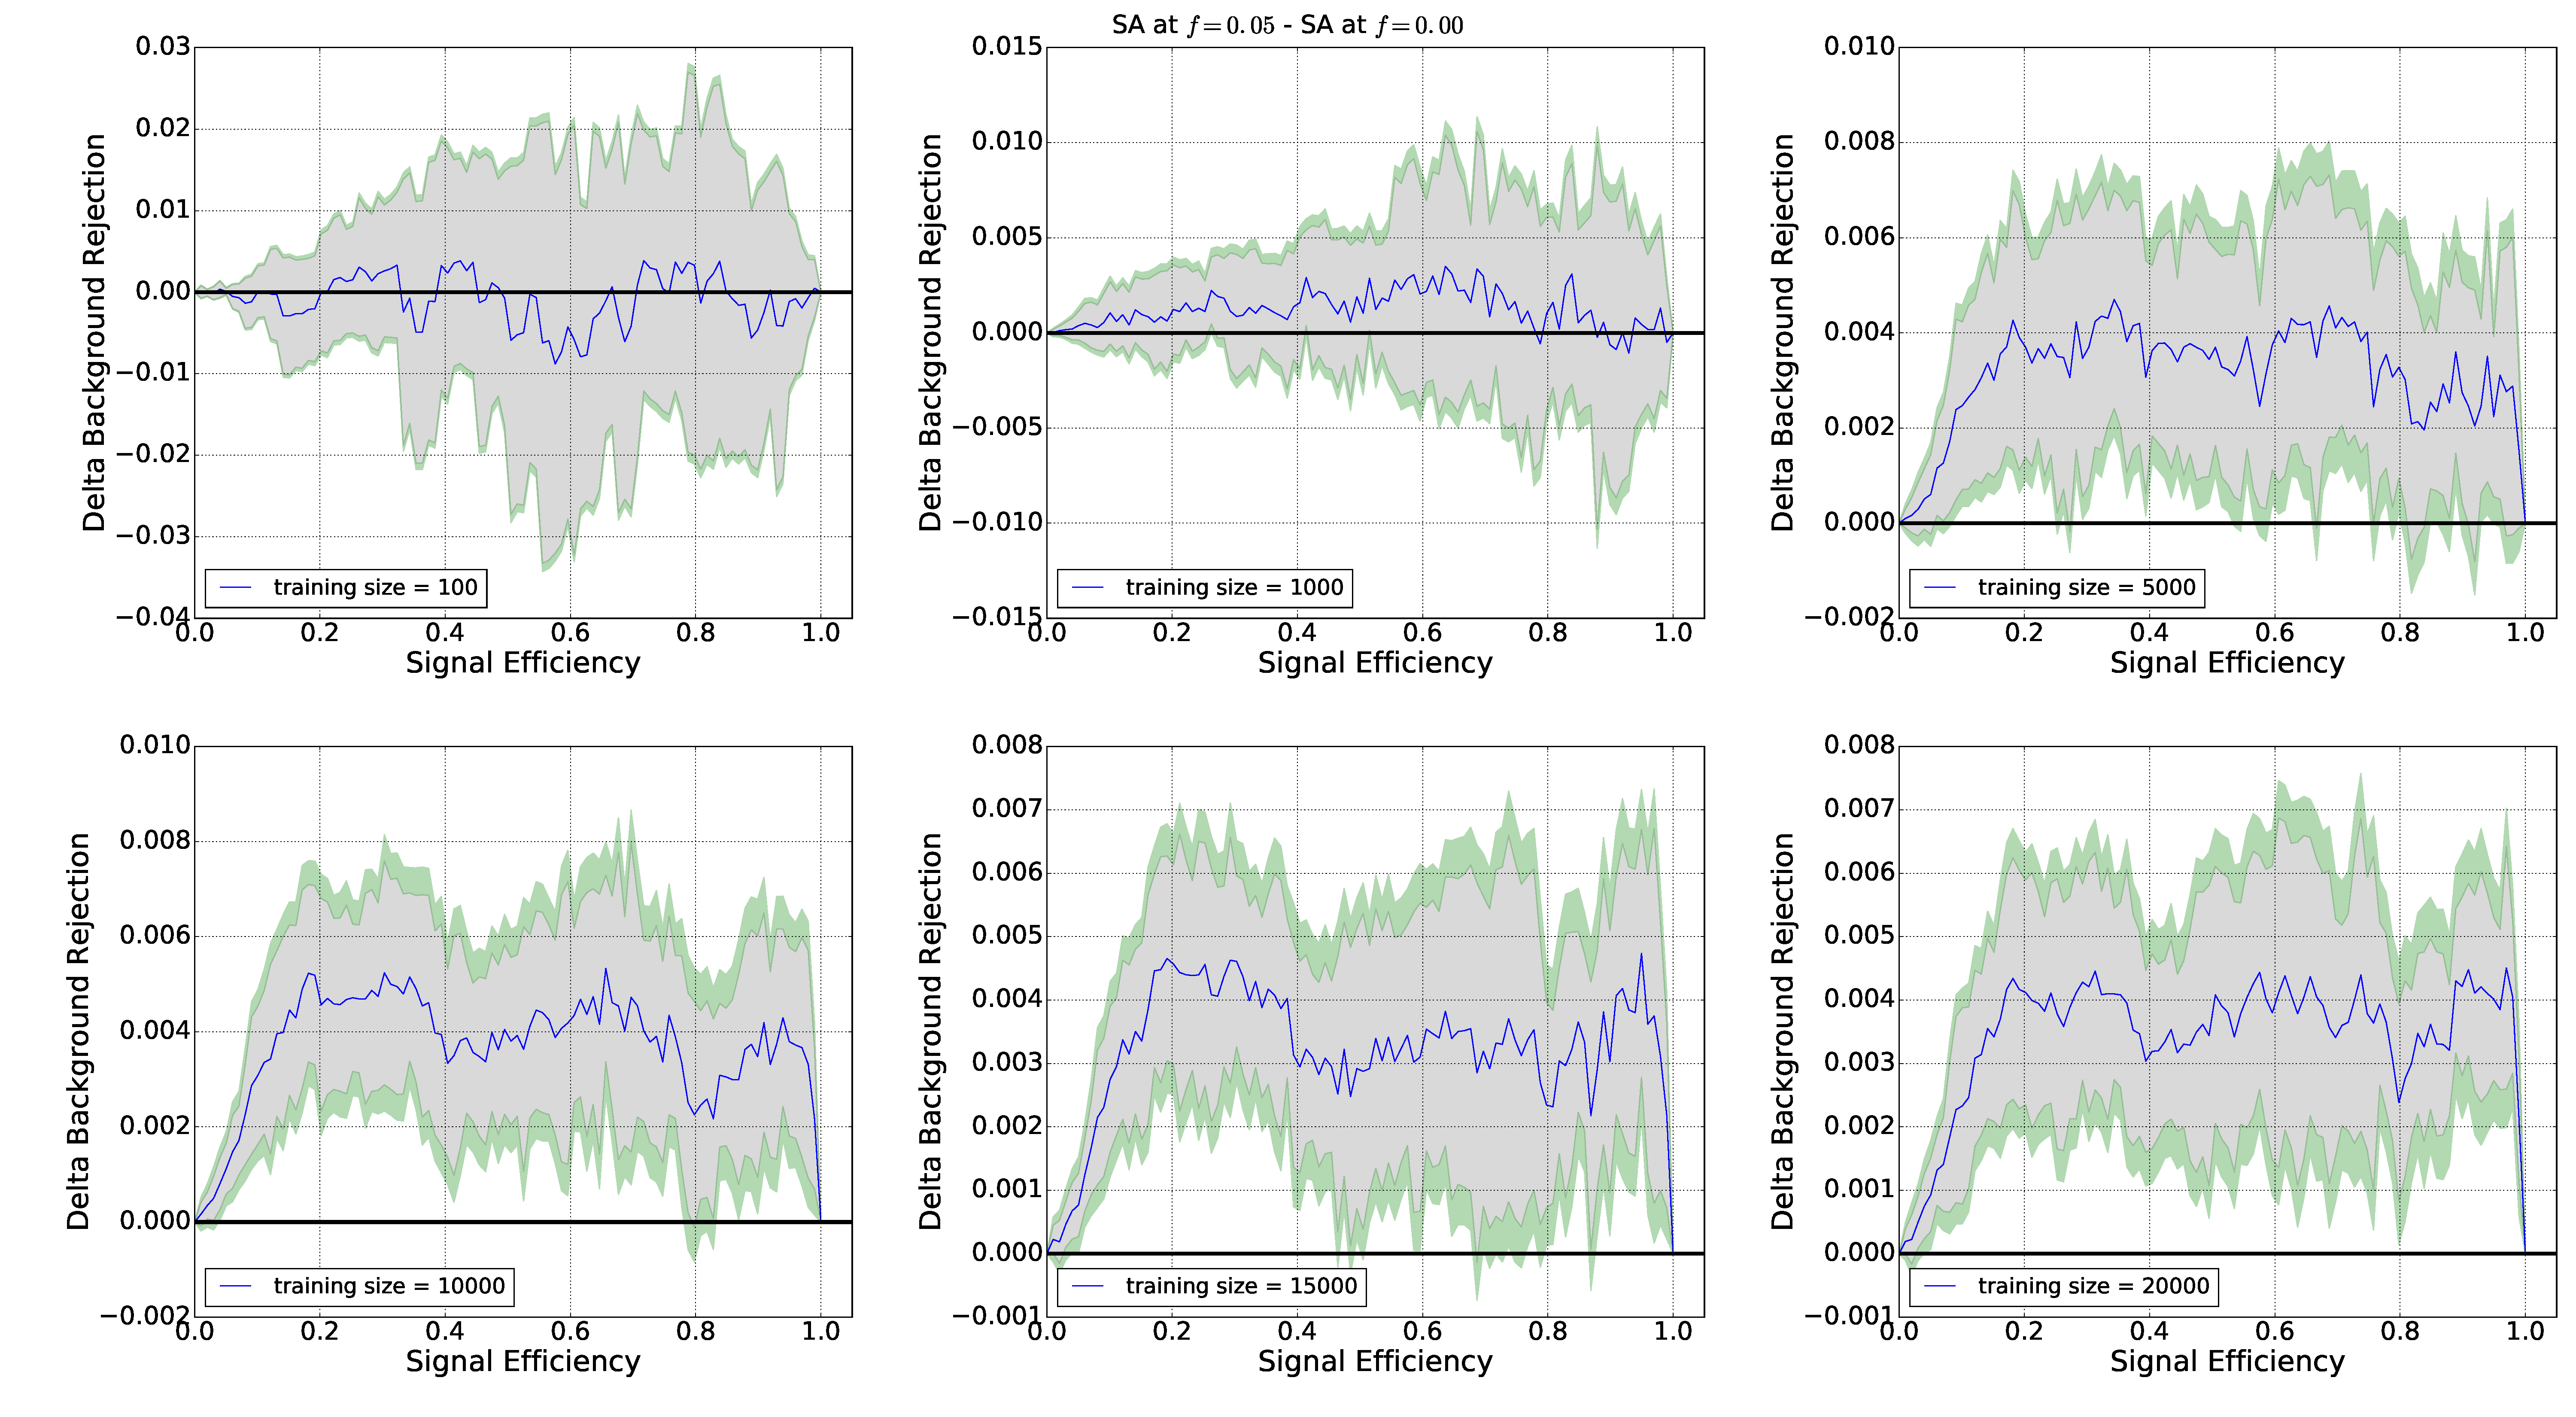
\includegraphics[width=0.8\paperwidth]{SA--SA_L5}
% \end{adjustbox}
\caption{Difference between the ROC curves between the true ground state configuration and the $f=0.05$ composite classifier from SA.}
\label{fig:SA_GS_SA_L3_droc}
\end{figure}
\clearpage
\begin{figure}[h]
\centering
% \begin{adjustbox}{center}
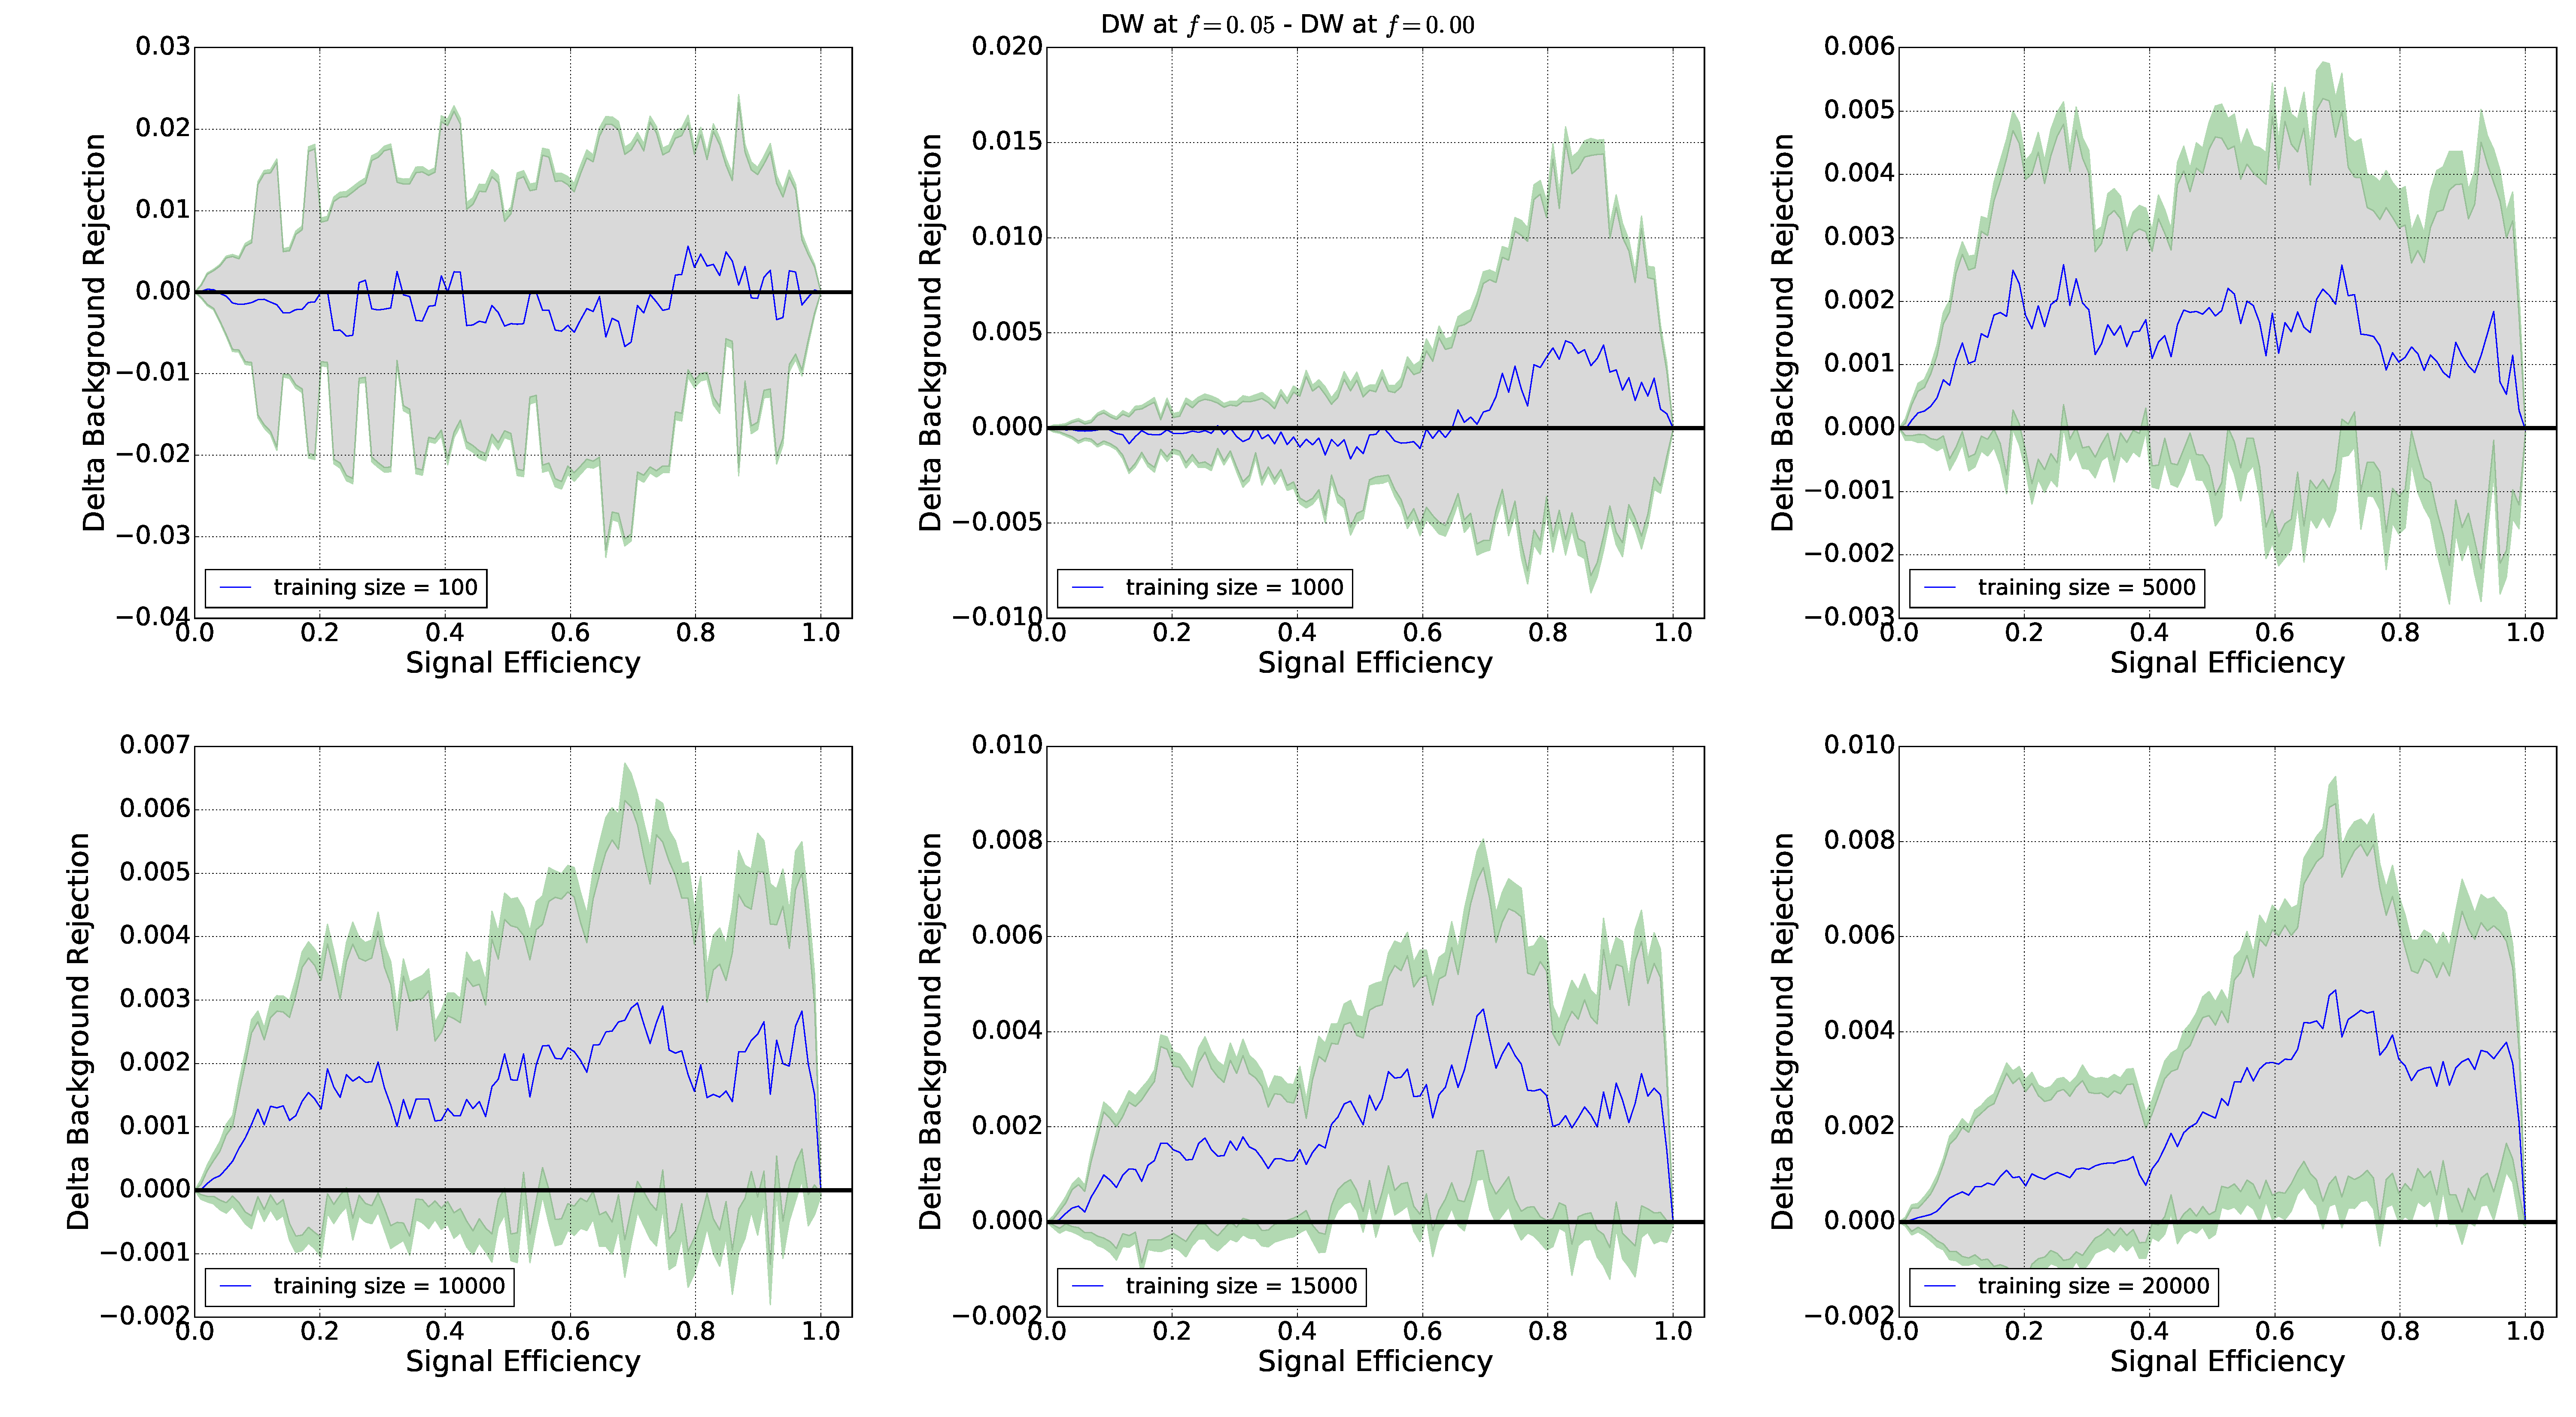
\includegraphics[width=0.8\paperwidth]{DW--DW_L5}
% \end{adjustbox}
\caption{Difference between the ROC curves between the minimum energy state returned by DW and the $f=0.05$ composite classifier from DW.}
\label{fig:DW_GS_DW_L3_droc}
\end{figure}

\bibliography{refs.bib}
% \begin{thebibliography}{10}
% \expandafter\ifx\csname url\endcsname\relax
%   \def\url#1{\texttt{#1}}\fi
% \expandafter\ifx\csname urlprefix\endcsname\relax\def\urlprefix{URL }\fi
% \providecommand{\bibinfo}[2]{#2}
% \providecommand{\eprint}[2][]{\url{#2}}

% \bibitem{Sherpa:2009}
% T~Gleisberg, Stefan H{\"o}che, F~Krauss, M~Sch{\"o}nherr, S~Schumann,
%   F~Siegert, and J~Winter.
% \newblock Event generation with sherpa 1.1.
% \newblock {\em Journal of High Energy Physics}, 2009(02):007, 2009.

% \bibitem{Pythia:2006}
% Torbj{\"o}rn Sj{\"o}strand, Stephen Mrenna, and Peter Skands.
% \newblock Pythia 6.4 physics and manual.
% \newblock {\em Journal of High Energy Physics}, 2006(05):026, 2006.
% \end{thebibliography} 


\end{document}
